\documentclass[a4paper]{report}

%%%%% NEW MATH DEFINITIONS %%%%%

\usepackage{amsmath,amsfonts,bm}

% Mark sections of captions for referring to divisions of figures
\newcommand{\figleft}{{\em (Left)}}
\newcommand{\figcenter}{{\em (Center)}}
\newcommand{\figright}{{\em (Right)}}
\newcommand{\figtop}{{\em (Top)}}
\newcommand{\figbottom}{{\em (Bottom)}}
\newcommand{\captiona}{{\em (a)}}
\newcommand{\captionb}{{\em (b)}}
\newcommand{\captionc}{{\em (c)}}
\newcommand{\captiond}{{\em (d)}}

% Highlight a newly defined term
\newcommand{\newterm}[1]{{\bf #1}}


% Figure reference, lower-case.
\def\figref#1{figure~\ref{#1}}
% Figure reference, capital. For start of sentence
\def\Figref#1{Figure~\ref{#1}}
\def\twofigref#1#2{figures \ref{#1} and \ref{#2}}
\def\quadfigref#1#2#3#4{figures \ref{#1}, \ref{#2}, \ref{#3} and \ref{#4}}
% Section reference, lower-case.
\def\secref#1{section~\ref{#1}}
% Section reference, capital.
\def\Secref#1{Section~\ref{#1}}
% Reference to two sections.
\def\twosecrefs#1#2{sections \ref{#1} and \ref{#2}}
% Reference to three sections.
\def\secrefs#1#2#3{sections \ref{#1}, \ref{#2} and \ref{#3}}
% Reference to an equation, lower-case.
\def\eqref#1{equation~\ref{#1}}
% Reference to an equation, upper case
\def\Eqref#1{Equation~\ref{#1}}
% A raw reference to an equation---avoid using if possible
\def\plaineqref#1{\ref{#1}}
% Reference to a chapter, lower-case.
\def\chapref#1{chapter~\ref{#1}}
% Reference to an equation, upper case.
\def\Chapref#1{Chapter~\ref{#1}}
% Reference to a range of chapters
\def\rangechapref#1#2{chapters\ref{#1}--\ref{#2}}
% Reference to an algorithm, lower-case.
\def\algref#1{algorithm~\ref{#1}}
% Reference to an algorithm, upper case.
\def\Algref#1{Algorithm~\ref{#1}}
\def\twoalgref#1#2{algorithms \ref{#1} and \ref{#2}}
\def\Twoalgref#1#2{Algorithms \ref{#1} and \ref{#2}}
% Reference to a part, lower case
\def\partref#1{part~\ref{#1}}
% Reference to a part, upper case
\def\Partref#1{Part~\ref{#1}}
\def\twopartref#1#2{parts \ref{#1} and \ref{#2}}

\def\ceil#1{\lceil #1 \rceil}
\def\floor#1{\lfloor #1 \rfloor}
\def\1{\bm{1}}
\newcommand{\train}{\mathcal{D}}
\newcommand{\valid}{\mathcal{D_{\mathrm{valid}}}}
\newcommand{\test}{\mathcal{D_{\mathrm{test}}}}

\def\eps{{\epsilon}}


% Random variables
\def\reta{{\textnormal{$\eta$}}}
\def\ra{{\textnormal{a}}}
\def\rb{{\textnormal{b}}}
\def\rc{{\textnormal{c}}}
\def\rd{{\textnormal{d}}}
\def\re{{\textnormal{e}}}
\def\rf{{\textnormal{f}}}
\def\rg{{\textnormal{g}}}
\def\rh{{\textnormal{h}}}
\def\ri{{\textnormal{i}}}
\def\rj{{\textnormal{j}}}
\def\rk{{\textnormal{k}}}
\def\rl{{\textnormal{l}}}
% rm is already a command, just don't name any random variables m
\def\rn{{\textnormal{n}}}
\def\ro{{\textnormal{o}}}
\def\rp{{\textnormal{p}}}
\def\rq{{\textnormal{q}}}
\def\rr{{\textnormal{r}}}
\def\rs{{\textnormal{s}}}
\def\rt{{\textnormal{t}}}
\def\ru{{\textnormal{u}}}
\def\rv{{\textnormal{v}}}
\def\rw{{\textnormal{w}}}
\def\rx{{\textnormal{x}}}
\def\ry{{\textnormal{y}}}
\def\rz{{\textnormal{z}}}

% Random vectors
\def\rvepsilon{{\mathbf{\epsilon}}}
\def\rvtheta{{\mathbf{\theta}}}
\def\rva{{\mathbf{a}}}
\def\rvb{{\mathbf{b}}}
\def\rvc{{\mathbf{c}}}
\def\rvd{{\mathbf{d}}}
\def\rve{{\mathbf{e}}}
\def\rvf{{\mathbf{f}}}
\def\rvg{{\mathbf{g}}}
\def\rvh{{\mathbf{h}}}
\def\rvu{{\mathbf{i}}}
\def\rvj{{\mathbf{j}}}
\def\rvk{{\mathbf{k}}}
\def\rvl{{\mathbf{l}}}
\def\rvm{{\mathbf{m}}}
\def\rvn{{\mathbf{n}}}
\def\rvo{{\mathbf{o}}}
\def\rvp{{\mathbf{p}}}
\def\rvq{{\mathbf{q}}}
\def\rvr{{\mathbf{r}}}
\def\rvs{{\mathbf{s}}}
\def\rvt{{\mathbf{t}}}
\def\rvu{{\mathbf{u}}}
\def\rvv{{\mathbf{v}}}
\def\rvw{{\mathbf{w}}}
\def\rvx{{\mathbf{x}}}
\def\rvy{{\mathbf{y}}}
\def\rvz{{\mathbf{z}}}

% Elements of random vectors
\def\erva{{\textnormal{a}}}
\def\ervb{{\textnormal{b}}}
\def\ervc{{\textnormal{c}}}
\def\ervd{{\textnormal{d}}}
\def\erve{{\textnormal{e}}}
\def\ervf{{\textnormal{f}}}
\def\ervg{{\textnormal{g}}}
\def\ervh{{\textnormal{h}}}
\def\ervi{{\textnormal{i}}}
\def\ervj{{\textnormal{j}}}
\def\ervk{{\textnormal{k}}}
\def\ervl{{\textnormal{l}}}
\def\ervm{{\textnormal{m}}}
\def\ervn{{\textnormal{n}}}
\def\ervo{{\textnormal{o}}}
\def\ervp{{\textnormal{p}}}
\def\ervq{{\textnormal{q}}}
\def\ervr{{\textnormal{r}}}
\def\ervs{{\textnormal{s}}}
\def\ervt{{\textnormal{t}}}
\def\ervu{{\textnormal{u}}}
\def\ervv{{\textnormal{v}}}
\def\ervw{{\textnormal{w}}}
\def\ervx{{\textnormal{x}}}
\def\ervy{{\textnormal{y}}}
\def\ervz{{\textnormal{z}}}

% Random matrices
\def\rmA{{\mathbf{A}}}
\def\rmB{{\mathbf{B}}}
\def\rmC{{\mathbf{C}}}
\def\rmD{{\mathbf{D}}}
\def\rmE{{\mathbf{E}}}
\def\rmF{{\mathbf{F}}}
\def\rmG{{\mathbf{G}}}
\def\rmH{{\mathbf{H}}}
\def\rmI{{\mathbf{I}}}
\def\rmJ{{\mathbf{J}}}
\def\rmK{{\mathbf{K}}}
\def\rmL{{\mathbf{L}}}
\def\rmM{{\mathbf{M}}}
\def\rmN{{\mathbf{N}}}
\def\rmO{{\mathbf{O}}}
\def\rmP{{\mathbf{P}}}
\def\rmQ{{\mathbf{Q}}}
\def\rmR{{\mathbf{R}}}
\def\rmS{{\mathbf{S}}}
\def\rmT{{\mathbf{T}}}
\def\rmU{{\mathbf{U}}}
\def\rmV{{\mathbf{V}}}
\def\rmW{{\mathbf{W}}}
\def\rmX{{\mathbf{X}}}
\def\rmY{{\mathbf{Y}}}
\def\rmZ{{\mathbf{Z}}}

% Elements of random matrices
\def\ermA{{\textnormal{A}}}
\def\ermB{{\textnormal{B}}}
\def\ermC{{\textnormal{C}}}
\def\ermD{{\textnormal{D}}}
\def\ermE{{\textnormal{E}}}
\def\ermF{{\textnormal{F}}}
\def\ermG{{\textnormal{G}}}
\def\ermH{{\textnormal{H}}}
\def\ermI{{\textnormal{I}}}
\def\ermJ{{\textnormal{J}}}
\def\ermK{{\textnormal{K}}}
\def\ermL{{\textnormal{L}}}
\def\ermM{{\textnormal{M}}}
\def\ermN{{\textnormal{N}}}
\def\ermO{{\textnormal{O}}}
\def\ermP{{\textnormal{P}}}
\def\ermQ{{\textnormal{Q}}}
\def\ermR{{\textnormal{R}}}
\def\ermS{{\textnormal{S}}}
\def\ermT{{\textnormal{T}}}
\def\ermU{{\textnormal{U}}}
\def\ermV{{\textnormal{V}}}
\def\ermW{{\textnormal{W}}}
\def\ermX{{\textnormal{X}}}
\def\ermY{{\textnormal{Y}}}
\def\ermZ{{\textnormal{Z}}}

% Vectors
\def\vzero{{\bm{0}}}
\def\vone{{\bm{1}}}
\def\vmu{{\bm{\mu}}}
\def\vtheta{{\bm{\theta}}}
\def\va{{\bm{a}}}
\def\vb{{\bm{b}}}
\def\vc{{\bm{c}}}
\def\vd{{\bm{d}}}
\def\ve{{\bm{e}}}
\def\vf{{\bm{f}}}
\def\vg{{\bm{g}}}
\def\vh{{\bm{h}}}
\def\vi{{\bm{i}}}
\def\vj{{\bm{j}}}
\def\vk{{\bm{k}}}
\def\vl{{\bm{l}}}
\def\vm{{\bm{m}}}
\def\vn{{\bm{n}}}
\def\vo{{\bm{o}}}
\def\vp{{\bm{p}}}
\def\vq{{\bm{q}}}
\def\vr{{\bm{r}}}
\def\vs{{\bm{s}}}
\def\vt{{\bm{t}}}
\def\vu{{\bm{u}}}
\def\vv{{\bm{v}}}
\def\vw{{\bm{w}}}
\def\vx{{\bm{x}}}
\def\vy{{\bm{y}}}
\def\vz{{\bm{z}}}

% Elements of vectors
\def\evalpha{{\alpha}}
\def\evbeta{{\beta}}
\def\evepsilon{{\epsilon}}
\def\evlambda{{\lambda}}
\def\evomega{{\omega}}
\def\evmu{{\mu}}
\def\evpsi{{\psi}}
\def\evsigma{{\sigma}}
\def\evtheta{{\theta}}
\def\eva{{a}}
\def\evb{{b}}
\def\evc{{c}}
\def\evd{{d}}
\def\eve{{e}}
\def\evf{{f}}
\def\evg{{g}}
\def\evh{{h}}
\def\evi{{i}}
\def\evj{{j}}
\def\evk{{k}}
\def\evl{{l}}
\def\evm{{m}}
\def\evn{{n}}
\def\evo{{o}}
\def\evp{{p}}
\def\evq{{q}}
\def\evr{{r}}
\def\evs{{s}}
\def\evt{{t}}
\def\evu{{u}}
\def\evv{{v}}
\def\evw{{w}}
\def\evx{{x}}
\def\evy{{y}}
\def\evz{{z}}

% Matrix
\def\mA{{\bm{A}}}
\def\mB{{\bm{B}}}
\def\mC{{\bm{C}}}
\def\mD{{\bm{D}}}
\def\mE{{\bm{E}}}
\def\mF{{\bm{F}}}
\def\mG{{\bm{G}}}
\def\mH{{\bm{H}}}
\def\mI{{\bm{I}}}
\def\mJ{{\bm{J}}}
\def\mK{{\bm{K}}}
\def\mL{{\bm{L}}}
\def\mM{{\bm{M}}}
\def\mN{{\bm{N}}}
\def\mO{{\bm{O}}}
\def\mP{{\bm{P}}}
\def\mQ{{\bm{Q}}}
\def\mR{{\bm{R}}}
\def\mS{{\bm{S}}}
\def\mT{{\bm{T}}}
\def\mU{{\bm{U}}}
\def\mV{{\bm{V}}}
\def\mW{{\bm{W}}}
\def\mX{{\bm{X}}}
\def\mY{{\bm{Y}}}
\def\mZ{{\bm{Z}}}
\def\mBeta{{\bm{\beta}}}
\def\mPhi{{\bm{\Phi}}}
\def\mLambda{{\bm{\Lambda}}}
\def\mSigma{{\bm{\Sigma}}}

% Tensor
\DeclareMathAlphabet{\mathsfit}{\encodingdefault}{\sfdefault}{m}{sl}
\SetMathAlphabet{\mathsfit}{bold}{\encodingdefault}{\sfdefault}{bx}{n}
\newcommand{\tens}[1]{\bm{\mathsfit{#1}}}
\def\tA{{\tens{A}}}
\def\tB{{\tens{B}}}
\def\tC{{\tens{C}}}
\def\tD{{\tens{D}}}
\def\tE{{\tens{E}}}
\def\tF{{\tens{F}}}
\def\tG{{\tens{G}}}
\def\tH{{\tens{H}}}
\def\tI{{\tens{I}}}
\def\tJ{{\tens{J}}}
\def\tK{{\tens{K}}}
\def\tL{{\tens{L}}}
\def\tM{{\tens{M}}}
\def\tN{{\tens{N}}}
\def\tO{{\tens{O}}}
\def\tP{{\tens{P}}}
\def\tQ{{\tens{Q}}}
\def\tR{{\tens{R}}}
\def\tS{{\tens{S}}}
\def\tT{{\tens{T}}}
\def\tU{{\tens{U}}}
\def\tV{{\tens{V}}}
\def\tW{{\tens{W}}}
\def\tX{{\tens{X}}}
\def\tY{{\tens{Y}}}
\def\tZ{{\tens{Z}}}


% Graph
\def\gA{{\mathcal{A}}}
\def\gB{{\mathcal{B}}}
\def\gC{{\mathcal{C}}}
\def\gD{{\mathcal{D}}}
\def\gE{{\mathcal{E}}}
\def\gF{{\mathcal{F}}}
\def\gG{{\mathcal{G}}}
\def\gH{{\mathcal{H}}}
\def\gI{{\mathcal{I}}}
\def\gJ{{\mathcal{J}}}
\def\gK{{\mathcal{K}}}
\def\gL{{\mathcal{L}}}
\def\gM{{\mathcal{M}}}
\def\gN{{\mathcal{N}}}
\def\gO{{\mathcal{O}}}
\def\gP{{\mathcal{P}}}
\def\gQ{{\mathcal{Q}}}
\def\gR{{\mathcal{R}}}
\def\gS{{\mathcal{S}}}
\def\gT{{\mathcal{T}}}
\def\gU{{\mathcal{U}}}
\def\gV{{\mathcal{V}}}
\def\gW{{\mathcal{W}}}
\def\gX{{\mathcal{X}}}
\def\gY{{\mathcal{Y}}}
\def\gZ{{\mathcal{Z}}}

% Sets
\def\sA{{\mathbb{A}}}
\def\sB{{\mathbb{B}}}
\def\sC{{\mathbb{C}}}
\def\sD{{\mathbb{D}}}
% Don't use a set called E, because this would be the same as our symbol
% for expectation.
\def\sF{{\mathbb{F}}}
\def\sG{{\mathbb{G}}}
\def\sH{{\mathbb{H}}}
\def\sI{{\mathbb{I}}}
\def\sJ{{\mathbb{J}}}
\def\sK{{\mathbb{K}}}
\def\sL{{\mathbb{L}}}
\def\sM{{\mathbb{M}}}
\def\sN{{\mathbb{N}}}
\def\sO{{\mathbb{O}}}
\def\sP{{\mathbb{P}}}
\def\sQ{{\mathbb{Q}}}
\def\sR{{\mathbb{R}}}
\def\sS{{\mathbb{S}}}
\def\sT{{\mathbb{T}}}
\def\sU{{\mathbb{U}}}
\def\sV{{\mathbb{V}}}
\def\sW{{\mathbb{W}}}
\def\sX{{\mathbb{X}}}
\def\sY{{\mathbb{Y}}}
\def\sZ{{\mathbb{Z}}}

% Entries of a matrix
\def\emLambda{{\Lambda}}
\def\emA{{A}}
\def\emB{{B}}
\def\emC{{C}}
\def\emD{{D}}
\def\emE{{E}}
\def\emF{{F}}
\def\emG{{G}}
\def\emH{{H}}
\def\emI{{I}}
\def\emJ{{J}}
\def\emK{{K}}
\def\emL{{L}}
\def\emM{{M}}
\def\emN{{N}}
\def\emO{{O}}
\def\emP{{P}}
\def\emQ{{Q}}
\def\emR{{R}}
\def\emS{{S}}
\def\emT{{T}}
\def\emU{{U}}
\def\emV{{V}}
\def\emW{{W}}
\def\emX{{X}}
\def\emY{{Y}}
\def\emZ{{Z}}
\def\emSigma{{\Sigma}}

% entries of a tensor
% Same font as tensor, without \bm wrapper
\newcommand{\etens}[1]{\mathsfit{#1}}
\def\etLambda{{\etens{\Lambda}}}
\def\etA{{\etens{A}}}
\def\etB{{\etens{B}}}
\def\etC{{\etens{C}}}
\def\etD{{\etens{D}}}
\def\etE{{\etens{E}}}
\def\etF{{\etens{F}}}
\def\etG{{\etens{G}}}
\def\etH{{\etens{H}}}
\def\etI{{\etens{I}}}
\def\etJ{{\etens{J}}}
\def\etK{{\etens{K}}}
\def\etL{{\etens{L}}}
\def\etM{{\etens{M}}}
\def\etN{{\etens{N}}}
\def\etO{{\etens{O}}}
\def\etP{{\etens{P}}}
\def\etQ{{\etens{Q}}}
\def\etR{{\etens{R}}}
\def\etS{{\etens{S}}}
\def\etT{{\etens{T}}}
\def\etU{{\etens{U}}}
\def\etV{{\etens{V}}}
\def\etW{{\etens{W}}}
\def\etX{{\etens{X}}}
\def\etY{{\etens{Y}}}
\def\etZ{{\etens{Z}}}

% The true underlying data generating distribution
\newcommand{\pdata}{p_{\rm{data}}}
% The empirical distribution defined by the training set
\newcommand{\ptrain}{\hat{p}_{\rm{data}}}
\newcommand{\Ptrain}{\hat{P}_{\rm{data}}}
% The model distribution
\newcommand{\pmodel}{p_{\rm{model}}}
\newcommand{\Pmodel}{P_{\rm{model}}}
\newcommand{\ptildemodel}{\tilde{p}_{\rm{model}}}
% Stochastic autoencoder distributions
\newcommand{\pencode}{p_{\rm{encoder}}}
\newcommand{\pdecode}{p_{\rm{decoder}}}
\newcommand{\precons}{p_{\rm{reconstruct}}}

\newcommand{\laplace}{\mathrm{Laplace}} % Laplace distribution

\newcommand{\E}{\mathbb{E}}
\newcommand{\Ls}{\mathcal{L}}
\newcommand{\R}{\mathbb{R}}
\newcommand{\emp}{\tilde{p}}
\newcommand{\lr}{\alpha}
\newcommand{\reg}{\lambda}
\newcommand{\rect}{\mathrm{rectifier}}
\newcommand{\softmax}{\mathrm{softmax}}
\newcommand{\sigmoid}{\sigma}
\newcommand{\softplus}{\zeta}
\newcommand{\KL}{D_{\mathrm{KL}}}
\newcommand{\Var}{\mathrm{Var}}
\newcommand{\standarderror}{\mathrm{SE}}
\newcommand{\Cov}{\mathrm{Cov}}
% Wolfram Mathworld says $L^2$ is for function spaces and $\ell^2$ is for vectors
% But then they seem to use $L^2$ for vectors throughout the site, and so does
% wikipedia.
\newcommand{\normlzero}{L^0}
\newcommand{\normlone}{L^1}
\newcommand{\normltwo}{L^2}
\newcommand{\normlp}{L^p}
\newcommand{\normmax}{L^\infty}

\newcommand{\parents}{Pa} % See usage in notation.tex. Chosen to match Daphne's book.

\DeclareMathOperator*{\argmax}{arg\,max}
\DeclareMathOperator*{\argmin}{arg\,min}

\DeclareMathOperator{\sign}{sign}
\DeclareMathOperator{\Tr}{Tr}
\let\ab\allowbreak


\usepackage[utf8]{inputenc}
\usepackage{caption}
\usepackage{subcaption}
\usepackage{graphicx}
\usepackage{biblatex}
\usepackage{setspace}

\doublespacing
\usepackage{amsmath}
\usepackage{amssymb}
\usepackage{dsfont}
\usepackage{array}
\usepackage{booktabs}
\usepackage{nameref}
\usepackage{mathtools}
\usepackage[stretch=10]{microtype}
\usepackage{acronym}
\usepackage{xcolor}
\usepackage{colortbl}
\usepackage{multirow}
\usepackage{xspace}
\usepackage{url}

\usepackage{anyfontsize}
\newcommand{\eg}{e.g.,\xspace}
\newcommand{\bigeg}{E.g.,\xspace}
\newcommand{\etal}{\textit{et~al.\xspace}}
\newcommand{\etc}{etc.\@\xspace}
\newcommand{\ie}{i.e.,\xspace}
\newcommand{\bigie}{I.e.,\xspace}
\usepackage[symbol]{footmisc}


% Please leave these options as they are
\usepackage{hyperref}
\usepackage{cleveref}
\hypersetup{
    colorlinks=true,
    linkcolor=red,
    filecolor=magenta,
    urlcolor=blue,
    citecolor=purple,
    pdftitle={Overleaf Example},
    pdfpagemode=FullScreen,
    }


\def\smtt#1{\texttt{\textsc{#1}}}
\acrodef{WADE}[WADE]{Weighted Average Data Efficiency}
\acrodef{RNN}[RNN]{recurrent neural network}

\urldef\projecturl\url{https://hugocisneros.com/ALIFE-Paper-2020/}

\title{
{Unsupervised learning in complex systems}\\
{\large École normale supérieure}\\
% {\includegraphics{uni.jpg}}
}
\author{Hugo Cisneros}
\date{2022}

\addbibresource{lib1.bib}
\addbibresource{lib2.bib}
\addbibresource{lib3.bib}


\begin{document}
\maketitle

\tableofcontents

\chapter{Introduction}
\label{cha:introduction}
% Intro should be readable to a non expert

\section{Goal}

Complex systems are systems composed of many interconnected elements that 
interact with each other, often in non-linear ways, giving rise to emergent 
properties that cannot be explained by the properties of the individual 
elements alone. In many natural complex systems, learning is a key process that 
allows the system to adapt and evolve over time. 
In this thesis, we explore complex systems
as a framework for studying learning and adaptation in natural and artificial
systems. The aim of this thesis is to develop methods for studying and using
computations that take place in complex dynamical systems to eventually create
learning algorithms that require limited to no supervision. 
Complex systems are systems made up of many interacting components that often 
exhibit non-linear and emergent behaviors that cannot be fully understood by 
analyzing the individual parts of the system in isolation. They often exhibit 
features such as self-organization, adaptation, feedback loops, and the capacity
to undergo phase transitions, all of which can make them challenging to model and 
predict. Examples of complex systems that occur naturally include ecosystems, weather patterns, financial 
markets, social networks, and biological organisms.
This objective is broken down into the following subgoals:

\begin{enumerate}
  \item The first subgoal is to identify complex dynamical systems that have the 
  potential to display emergent open-ended growth, which refers to the ability of 
  a system to spontaneously generate new levels of complexity over time without 
  reaching a state of equilibrium. This growth is often associated with 
  evolutionary-like properties, such as variation, selection, and inheritance.
  There are many ways to define complex systems, and as
        illustrated in Figure \ref{fig:comparison_ca}, some may exhibit more
        interesting and promising behaviors than others. A cellular automaton (CA) 
        is an instance of a complex system that can be described as a grid of cells that can 
        take on a finite set of states and change their state over time according to a set 
        of rules that depend on the states of their neighboring cells. Interesting \acp{CA}, such 
        as the one shown in Figure \ref{fig:structured_sys}
        may be hard to find depending on how the
        search space is defined. The work presented in Chapter
        \ref{cha:meas-compl-evolv} aims to construct a metric of complexity
        that can help to identify interestingly behaving complex
        dynamical systems.
\begin{figure}[htbp]
  \centering
\begin{subfigure}[t]{.4\linewidth}
  \centering
  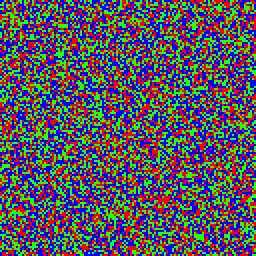
\includegraphics[width=\linewidth]{figures/disord2.png}
  \caption{A disordered \acl{CA}.}
 \label{fig:disordered_sys}
\end{subfigure}
\hspace{30pt}
\begin{subfigure}[t]{.4\linewidth}
  \centering
  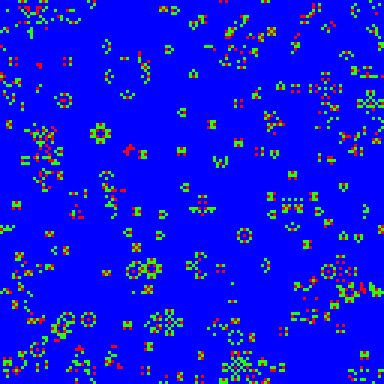
\includegraphics[width=\linewidth]{figures/micro4.png}
  \caption{A \acl{CA} with visible emergent structures.}
  \label{fig:structured_sys}
\end{subfigure}
\caption{Two examples of complex systems (\acf{CA}) with different behavior
  types. \ref{fig:structured_sys} and \ref{fig:disordered_sys} show a single state 
  of a randomly initialized 2D \ac{CA} simulated for a fixed number of steps. Some \acp{CA} 
  appear more promising than others for the design of
  unsupervised learning systems because of their emergent complex structures
  (visible in \ref{fig:structured_sys}), whereas the \ac{CA} in
  \ref{fig:disordered_sys} seems to behave randomly.}
  \label{fig:comparison_ca}
\end{figure}

  \item The second subgoal is to measure the fraction of systems that have the most complex and rapidly
        evolving behavior. Defining these notions is also part of the goal.
        This subgoal is distinct from the first one, which focuses on complex system design in 
        general. Instead, this subgoal involves establishing approaches to evaluate growth 
        in complexity.
        We believe that systems with the most complex and rapidly
        evolving behavior are promising for further use since
        they may exhibit open-ended complexity growth. In Chapters
        \ref{cha:meas-compl-evolv} and \ref{cha:visu-comp-large}, we present
        different methods to measure evolving complexity and understand when the
        complexity increases over time. Chapter \ref{cha:visu-comp-large} of this thesis is dedicated to investigating the importance of multiscale analysis for the complexity of
        cellular automata, which is the process of studying a system at different levels of detail or resolution.   Additionally, we identify complex systems with behavior that
        changes when we manipulate the scale of the system, either by increasing or decreasing its size.
\begin{figure}[htbp]
  \centering
 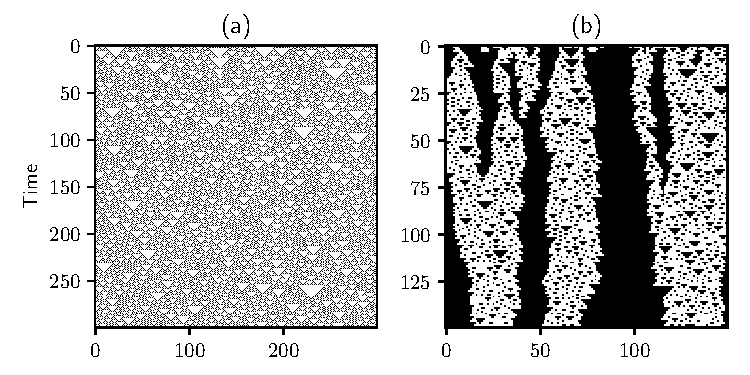
\includegraphics[width=.9\linewidth]{figures/rule18_small}
 \caption{Filtering the behavior of elementary \acl{CA} rule 18. This
   uncovers a highly structured behavior with the propagation of area boundaries
   within the apparent randomness. (a) shows 300 timesteps
of a randomly initialized rule 18 simulation. Notice the complex structures made
visible in (b) with a filtering method. This Figure is discussed in more details in Chapter \ref{cha:visu-comp-large}.}
  \label{fig:rule_18}
\end{figure}

  \item Apply promising systems to challenging learning tasks where classical
        machine learning models may fail or become less efficient. The goal is to
        define various ways to apply evolving complex dynamical systems to some
        standard learning tasks and to find out if it improves the performance
        or efficiency of the learning algorithm. An example application that we
        explore in Chapter \ref{cha:learn-effic-compl} is illustrated in
        Figure~\ref{fig:ca_lm}, where a \ac{CA} is used to implement a language
        model, a probabilistic model that is used to generate text to complete
        sentences. In Chapter \ref{cha:background}, we explore the similarities
        between \acp{CA} networks and highlight the numerous potential applications of \acp{CA}.
\begin{figure}[htbp]
  \centering
  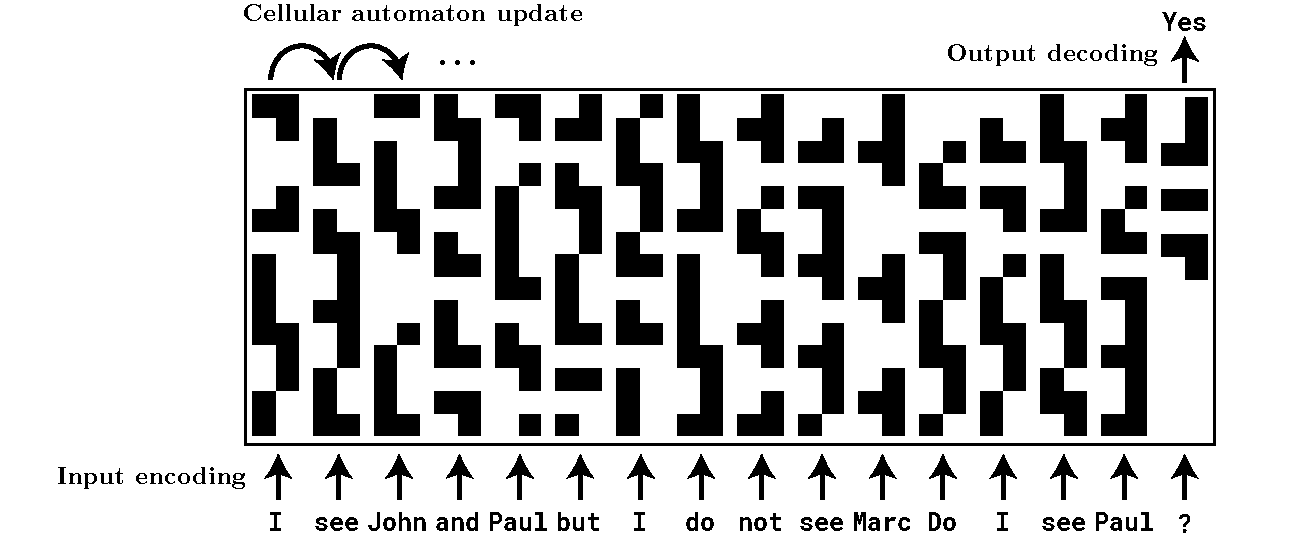
\includegraphics[width=\linewidth]{figures/ca_lm}
  \caption{An example of using a \acl{CA} and reservoir computing to implement a
    language model. Tokens are encoded within the \acl{CA} internal state. The
    \acl{CA} update rule is then applied and an output value is decoded from the
    final state. Each vertical bar represents two consecutive internal \ac{CA} states, which 
    are enriched with the encoded input.}
  \label{fig:ca_lm}
\end{figure}

\end{enumerate}

In this thesis, we do not focus our attention on what the machine learning
community commonly refers to as ``unsupervised learning'', that is, learning
structure from unlabeled data
\parencite{hintonUnsupervisedLearningFoundations1999}. In machine learning,
supervision refers to a label, a number, or a collection of numbers that
represents an expected outcome associated with some input data. Our goal is to
construct models that can develop autonomously without necessarily needing any external data or
interactions. Therefore, we first seek systems that behave that way on their
own and postpone the issue of learning to optimize a particular objective
function to the end of the thesis (Chapter \ref{cha:learn-effic-compl}). 
We are particularly interested in systems that can develop through
internal evolution rules without any input, which is the case for many complex
systems.

Throughout the thesis, we work toward achieving these goals, focusing on one
particular complex system: the \acl{CA} \parencite{vonneumannTheorySelfreproducingAutomata1966}. This model has been extensively studied
due to its simple definition and ability to simulate a wide range of complex
behaviors. We provide a detailed description of cellular automata in Section
\ref{sec:cellular-automata-sec}. This thesis provides new insights into the role
of learning in complex systems and open-ended evolution and demonstrates the
potential of cellular automata as a model for studying these phenomena.

\section{Motivation}\label{sec:motivation}

It is possible that some form of evolutionary mechanism may be necessary in
order to achieve advanced forms of artificial intelligence (AI), particularly 
if the goal is to create
intelligent systems that can adapt and learn in complex and changing
environments. Complex dynamical systems could be key to overcome the problems
with existing learning algorithms, such as difficulties in generalization,
robustness, or the ability to learn continuously
\parencite{parisiContinualLifelongLearning2019}. The natural intelligence of
biological systems seems to depend on emerging properties selected through
evolution. For example, biological life exhibits a pattern of major evolutionary
transitions in which autonomously replicating entities at the lower level merged to form a
single more complex corporate body
\parencite{lorenzEmergenceModularityBiological2011}. This is believed to have
occurred for the emergence of eukaryotic cells, as well as for multicellular
life \parencite{hammerschmidtLifeCyclesFitness2014}. All complex and diverse
biological entities have presumably emerged from a single common ancestor and,
even before, from inorganic components present on the surface of the Earth
\parencite{woeseUniversalAncestor1998, smithOriginsLifeBirth2000}.

So far, it remains uncertain which algorithmic characteristics might enable 
an artificial system to exhibit a path comparable to the natural evolutionary
process within its state space, which involves the transition from basic 
constituents to intricate entities. Producing emerging
phenomena similar to those of nature \emph{in silico} is a long-standing
challenge. There are many algorithms that attempt to mimic evolutionary
properties to solve particular tasks, called evolutionary algorithms
\parencite{fogelArtificialIntelligenceSimulated1966,
  ,millerDesigningNeuralNetworks1989, backOverviewEvolutionaryAlgorithms1993}.
However, many of these methods focus on searching the space of solutions using
high-level evolutionary mechanisms, such as genetic mutations and crossovers.
Although effective in solving precise tasks, these methods often obscure another
crucial component of natural evolution by using an explicit fitness function.

Most existing machine learning algorithms rely on the choice of an objective
function: a clearly defined mapping from the current state and parameters of a
model to a real value, which indicates the performance of that model. The
function depends on the objective of the model. For a supervised learning
problem, we may count the number of misclassified objects or the distance
between the predictions and the expected results. Even in unsupervised learning,
the family of algorithms used for learning from unlabeled data, objectives are
still central. For example, the well-known K-means clustering algorithm minimizes
the sum of square distances to cluster centers.

This reliance on objective functions creates two main issues: (i) the objective
is not always clearly defined or can be too broad for general-purpose
applications. For example, a possible objective function of a walking robot
could be ``not fall when stepping through its surrounding environment''. This
function is impractical to define and will vary greatly depending on the
parameters of the environment (e.g. depending on the terrain, malfunctioning or 
missing limbs of the robots). Indirect rewards such as ``head not touching the ground''
may help, but it does not cover all possible ways the model could fail. 
This problem of defining an objective is still present in our goal of designing
a general-purpose, autonomously developing learning algorithm.
Furthermore, (ii) using predefined functions as goals can be counterproductive
because, as many examples in nature demonstrate, robust paths to complex
objectives are often deceptive. They involve developing in unexpected directions
that may initially seem to be against the original goal
\parencite{stanleyWhyGreatnessCannot2015}.

In this thesis, the term \emph{unsupervised} refers to a form of learning with
no predefined objective. Like in natural evolution, we expect true unsupervised
algorithms to develop new features autonomously and become progressively more
complex over time. Such algorithms would regularly learn to solve problems on
their own without the need to be explicitly guided towards the problem solutions, 
thereby discovering robust
and diverse solutions to deceptive problems.


\section{Challenges}\label{sec:challenges}

\begin{figure}[htbp]
  \centering
  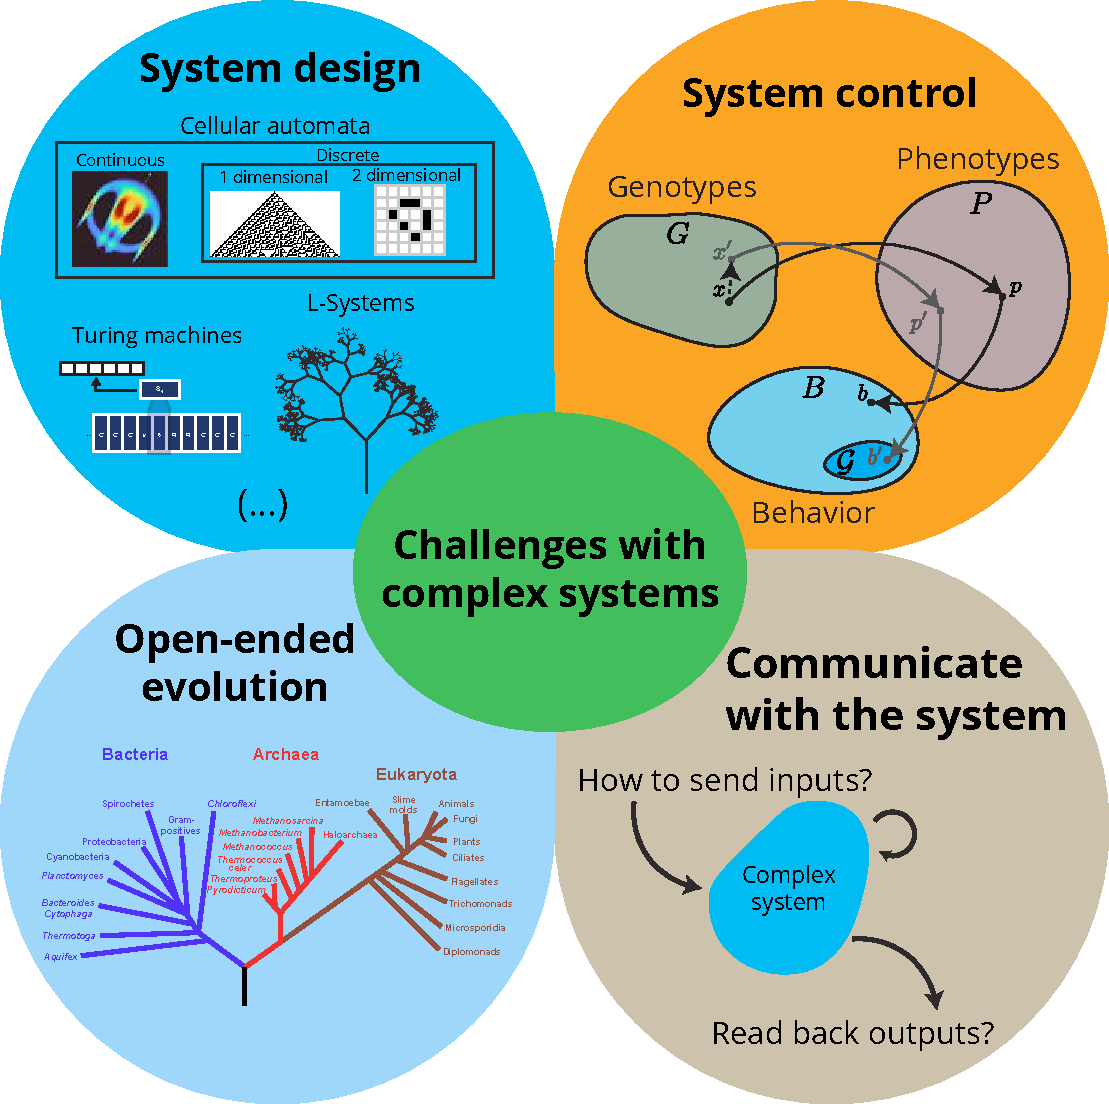
\includegraphics[width=.98\linewidth]{figures/challenges}
  \caption{The challenges of working with complex systems encountered across
    this thesis can be broken down in several categories. \textbf{(1)} The choice
    and design of the system, \textbf{(2)} the control of the system which
    involves understanding the complex mapping between a parameter space and the
    possibly unpredictable behavior of a system, \textbf{(3)} the search for
    open-ended evolution properties similar to the ones found in nature,
    \textbf{(4)} the issue of sending inputs and reading outputs from the
    internal state of a complex system. This illustration uses
    \href{https://commons.wikimedia.org/wiki/File:Lenia_icon4.png}{Lenia
      icon4.png} by Bert Wang-Chak Chan, licensed under
    \href{https://creativecommons.org/licenses/by-sa/4.0/}{CC BY 4.0}. }
  \label{fig:challenges}
\end{figure}

The study of complex systems presents a range of difficult challenges by itself
\parencite{sanmiguelChallengesComplexSystems2012}. 
The complexity of a system is an emergent property that arises from various factors, 
including its intricate structure, the number of elements it contains, how it functions, 
and how it responds to different kinds of external influences. These factors contribute 
to the overall complexity of the system, which could be measured in various ways.
For many complex systems, their emergent mechanisms are
poorly understood. We identify four main challenges associated with the study of
complex systems: (i) the questions of the design choices in defining and sampling a
complex system (section \ref{sec:design-compl-syst}), (ii) which will in turn define
their potential to support a form of open-ended evolution (section
\ref{sec:open-ended-evolution}) and (iii) how we can expect to build an interface to
communicate with it (section \ref{sec:compl-syst-inputs}), (iv) which is essential to
achieve some form of control of that system (section \ref{sec:compl-syst-contr}).

\subsection{Design of a complex system\label{sec:design-compl-syst}}

The first challenge is to construct a suitable complex system. The definition of a 
complex system is broad, and several systems with
interesting dynamics have been studied under that name. For example, abstract models such as L-Systems (formal grammars used to model the growth and development of organic structures),
Random Boolean networks (dynamical systems that consist of a fixed number of binary nodes 
that are randomly connected to each other and updated based on the state of its neighboring 
nodes), Turing machines (abstract deterministic computing machines consisting of a tape and 
a read-write head), and \Acfp{CA}. In this thesis, we
focus mainly on the last listed element: the \acl{CA}. There are multiple
benefits to working with this model. It is very simple to define, and its high
parallelism makes its implementation straightforward. Moreover, \acp{CA} have
shown the ability to simulate a wide range of complex behaviors
\parencite{wolframNewKindScience2002}.

Choosing the right complex system architecture is essential because it defines
the search space over which interesting and useful systems can be found.
Correctly parameterizing that space can also be challenging because too many
degrees of freedom make it difficult to search for and find good systems, while
too few might indicate a lack of expressivity. An example parameterization of
\ac{CA} with little expressivity is Langton's lambda parameter
\parencite{langtonComputationEdgeChaos1990}. At the other end of the spectrum, the
\ac{CA} rule is a simple parametrization with many degrees of freedom, which
makes it impractical.

Even when we limit ourselves to the study of \ac{CA}, many variants can be
considered. Cellular automata can have continuous or discrete states and operate
in continuous or discrete space. For discrete state and space cellular automata,
the number of states and the window of the update function can vary, as well as the
topology of the simulation space. We tackle this issue from various angles
across the thesis, exploring the question of rule definition in Chapter
\ref{cha:meas-compl-evolv}, the scale in Chapter \ref{cha:visu-comp-large} and
the connectivity pattern in Chapter \ref{cha:learn-effic-compl}.

\subsection{Complex systems control}\label{sec:compl-syst-contr}

\begin{figure}[htbp]
  \centering
  \begin{subfigure}[t]{.47\linewidth}
    \centering
    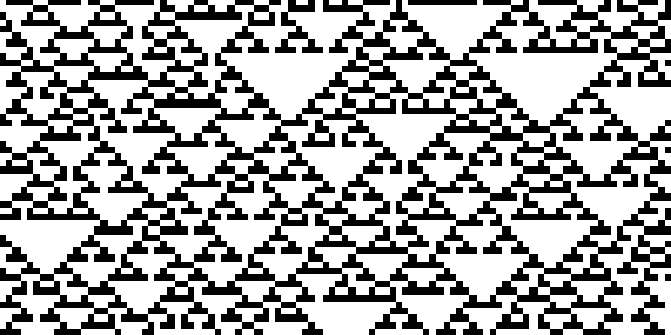
\includegraphics[width=.93\linewidth]{figures/ca_comp_a}
    \caption{\ac{CA} rule 22 on a tape of size 100, ran for 50 steps from a
      random initial state.}
    \label{fig:ca_comp_a}
  \end{subfigure}
  \hspace{10pt}
  \begin{subfigure}[t]{.47\linewidth}
    \centering
    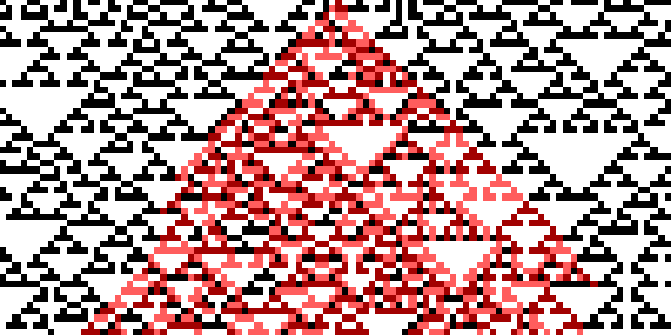
\includegraphics[width=.93\linewidth]{figures/ca_comp_b}
    \caption{\ac{CA} rule 22 on a tape of size 100, ran from a slightly
      different initial state. The cells different from Figure \ref{fig:ca_comp_a} are
      overlayed in red.}
    \label{fig:ca_comp_b}
  \end{subfigure}

  \caption{Comparison of the same 1 dimensional \ac{CA} ran from two initial conditions
    differing only by one cell. Each row is the state of the \ac{CA} at one time
    step. The effect of the small perturbation of initial conditions grows
    rapidly as the \ac{CA} evolves in time.}
  \label{fig:ca_comp}
\end{figure}


Even if we want complex systems that evolve in unexpected directions and grow in
an open-ended way without supervision, it may still be useful to steer them
locally towards specific targets. A major challenge that follows from this goal
is that many complex systems are chaotic. Deterministic dynamical systems can 
exhibit behavior that is extremely sensitive to their initial conditions. This sensitivity 
is sometimes referred to as chaos, where even tiny perturbations in the initial conditions 
can result in significantly different outcomes or trajectories. This is illustrated 
with a simple \ac{CA} rule in Figure \ref{fig:ca_comp}. 
Because of this property, it is often very hard to predict how a
given system will evolve over time, and therefore hard to steer its evolution
towards a particular final state or along a chosen trajectory. While it can be challenging 
to apply these systems to certain basic tasks, their ability to generate unexpected solutions 
to difficult problems is an advantage in developing open-ended systems. Such systems 
need to continually produce new and diverse solutions, without a 
predefined endpoint, and the sensitivity to initial conditions an advantage in 
achieving this goal.

This problem is also related to the issue of sending a control signal to a
complex system that depends on the choice of encoding for that signal. This
encoding can significantly impact the system's ability to respond to the control 
signal and generate the desired outcome. 

\subsection{Complex systems inputs and outputs\label{sec:compl-syst-inputs}}

Some of the complex systems we study in this thesis are closed systems. They do
not expect inputs or have any well-defined outputs. For example, \ac{CA} and
\ac{RBN} do not have a notion of inputs and outputs built into the model. They
are standalone objects that evolve according to a set of internal rules.

A common challenge for such systems is to define the inputs and outputs in a way
that preserves their internal dynamics. This is also connected to the control
problem of Section \ref{sec:compl-syst-contr}, because controlling a complex
system implies being able to send a control signal and read the current
state of the system.

Throughout this work, we use a framework called \emph{reservoir computing} (RC) for this 
purpose. Reservoir
computing allows one to harvest the internal computations of complex systems, or
\emph{read} information from its internal state by learning a linear regression
that maps that internal state to desired outputs (see Section
\ref{sec:res-models}).



\subsection{Open-ended evolution without
  objectives}\label{sec:open-ended-evolution}

Another challenge is posed by the lack of a clear objective in the design of
unsupervised learning systems. Even without an objective, it is still essential
to understand which complex systems to choose from all available options or how
to tune their parameters so that they behave in interesting ways. For example,
\acp{CA} such as the one shown in Figure \ref{fig:disordered_sys} are unlikely 
to be useful for constructing systems that demonstrate a growth of complexity 
due to their disordered nature in both space and time. As a result, they cannot
preserve information about the past.

Because our goal is to create a system that has the property of evolving in an
open-ended way, we need metrics that can help select systems. However, these metrics 
should not be used as an additional objective function, as doing so would result 
in the problems described in Section \ref{sec:motivation}. We address this 
challenge in particular
in Chapter~\ref{cha:meas-compl-evolv}, by designing a complexity metric that can
help select interesting complex systems, without relying on a specific
task-based performance score.

\section{Contributions}

The main contributions of this thesis are as follows.
\begin{enumerate}
  \item Our first contribution is a review of the literature (Chapter \ref{cha:literature-review})
        describing the connections between cellular automata
        and other complex systems, open-ended evolution, and neural networks.
        Studying these fields from a single point of view is a relatively novel
        endeavor, and we consider a review necessary to place the rest of our
        work in its context.

  \item Our second contribution is the development of a general complexity metric that can help identify
        complex systems with interesting behavior (Chapter \ref{cha:meas-compl-evolv}). Our findings were published in \cite{cisnerosEvolvingStructuresComplex2019}.

  \item The third contribution is the development of a coarse-graining method to visualize computations in
        cellular automata and other discrete systems with local interactions (Chapter \ref{cha:visu-comp-large}). Our findings were published in \cite{cisnerosVisualizingComputationLargescale2020}.

  \item Our fourth contribution is the introduction of a metric for learning efficiency for learning
        algorithms as well as a benchmark dataset of progressively harder
        language tasks (Chapter \ref{cha:learn-effic-compl}). Our findings were published in \cite{cisnerosBenchmarkingLearningEfficiency2022}.
\end{enumerate}

\section{Thesis overview}


Chapter \ref{cha:background} presents some background notions about complex
systems, cellular automata, and reservoir computing.

In Chapter \ref{cha:literature-review}, we review relevant methods and tools for
measuring the complexity of complex systems and using their computations for
various tasks.

Chapter \ref{cha:meas-compl-evolv} introduces a complexity metric that allows us 
to select complex systems with interesting behavior. The metric measures the
``novelty'' of the temporal states of a system compared to a reference one. We
built a dataset of interesting cellular automata to validate the quality of the
metric.

Chapter \ref{cha:visu-comp-large} addresses the question of large-scale complex
systems and the applicability of complexity metrics at multiple scales. We
propose three algorithms for the coarse-graining of cellular automata. This allows
us to reduce the size of large-scale systems while retaining the interesting parts
of the behavior.

Chapter \ref{cha:learn-effic-compl} presents a learning efficiency metric and a
dataset to measure the speed of learning of various systems. We show that
reservoir computing-based systems using cellular automata can be more efficient
than usual machine learning algorithms in constrained data and computation
settings.

Chapter \ref{cha:future_work} outlines potential avenues for further research in 
the field. It provides suggestions for how the current work could be expanded or 
improved, highlighting areas that require additional investigation to advance the 
understanding of the subject. We propose some experiments that could extend the 
potential applications of cellular automata, as well as a theoretical framework 
for learning in dynamical systems.

Finally, Chapter \ref{cha:conclusion} summarizes our contributions in this thesis. 

\section{Publications and software}

The thesis has led to the following publications.

\begin{itemize}
  \item \fullcite{cisnerosEvolvingStructuresComplex2019}
  \item \fullcite{cisnerosVisualizingComputationLargescale2020}
  \item \fullcite{cisnerosBenchmarkingLearningEfficiency2022}
\end{itemize}

The code to reproduce the experiments of all three publications is available on
GitHub: \url{https://github.com/hugcis/evolving-structures-in-complex-systems},
\url{https://github.com/hugcis/benchmark_learning_efficiency}. We also published a
dataset that we used for our benchmark in our last
publication. It is available at
\url{https://github.com/hugcis/incremental_tasks/}.

\chapter{Literature Review}
\label{cha:literature-review}

In this chapter, we review several fields associated with learning and complex
systems which served as a theoretical foundation for our work. The literature we
present also influenced and inspired this thesis. We begin by reviewing related
work on complexity measures for dynamical and complex systems (section
\ref{sec:measuring-complexity}). We also review works on defining and
understanding emergence (section \ref{sec:emergence}), evolutionary methods for
searching solutions in complex spaces (section \ref{sec:evol-algor}), methods
for constructing open-ended evolving systems (section
\ref{sec:open-ended-evolution-1}), and method for extracting and using the
computations happening within complex systems (section
\ref{sec:comp-with-compl}).

\section{Measuring complexity\label{sec:measuring-complexity}}

Measuring the complexity of a system is a fundamentally difficult task. Many
complex systems exhibit what Peter Grassberger calls \emph{self-generated
  complexity} \parencite{grassbergerQuantitativeTheorySelfgenerated1986}. This
means that the formulation of the problem is translationally invariant and the
observed structure arises from a spontaneous breakdown of translational
invariance. Unfortunately there is no universally accepted and formalized notion
of ``complexity'', even though most intuitively agree that it exists. For
example figure \ref{fig:three_eca_complex} shows three examples of behaviors
generated by 1D \acp{ECA}. Most people would consider the leftmost figure
\ref{fig:simple} as not complex. But, depending on one's definition of
complexity, the last picture could perhaps be labeled as complex.

\begin{figure}[htbp]
  \centering
  \begin{subfigure}[b]{.31\linewidth}
    \centering
    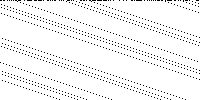
\includegraphics[width=\linewidth]{figures/three_simple_eca.png}
    \caption{}
   \label{fig:simple}
  \end{subfigure}
  \begin{subfigure}[b]{.31\linewidth}
    \centering
    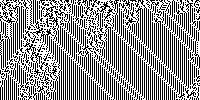
\includegraphics[width=\linewidth]{figures/three_complex_eca.png}
    \caption{}
   \label{fig:complex}
  \end{subfigure}
  \begin{subfigure}[b]{.31\linewidth}
    \centering
    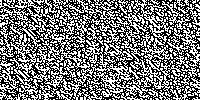
\includegraphics[width=\linewidth]{figures/three_random_eca.png}
    \caption{}
   \label{fig:random}
  \end{subfigure}
  \caption{Three 1D \aclp{CA} with qualitatively different behavior. The left
    (\ref{fig:simple}) and right (\ref{fig:random}) \acp{CA} are usually not
    defined as ``complex'', whereas the middle \ac{CA} (\ref{fig:complex})
    appears to be complex.}
  \label{fig:three_eca_complex}
\end{figure}

\begin{figure}[htbp]
  \centering
  \scalebox{1}{
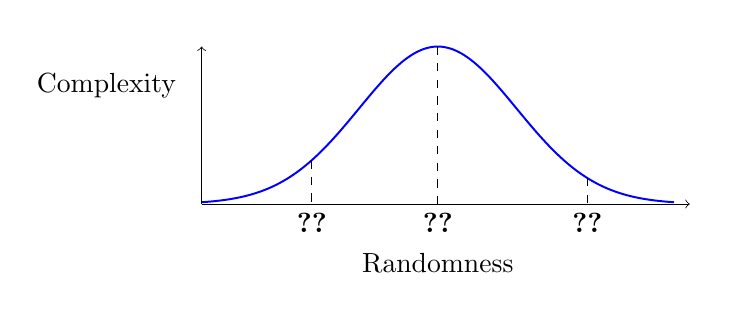
\begin{tikzpicture}
% define normal distribution function 'normaltwo'
\def\normaltwo{\x,{2*1/exp(((\x-3)^2)/2)}}

% input y parameter
\def\ya{4.9}
\def\fya{2*1/exp(((\ya-3)^2)/2)}

\def\yb{1.4}
\def\fyb{2*1/exp(((\yb-3)^2)/2)}

\def\yc{3}
\def\fyc{2*1/exp(((\yc-3)^2)/2)}

% Draw and label normal distribution function
\draw[color=blue,domain=0:6,smooth,samples=50, line width=0.25mm] plot (\normaltwo) node[right] {};

% Add dashed line dropping down from normal.
\draw[dashed] ({\ya},{\fya}) -- ({\ya},0) node[below] {\ref{fig:random}};
\draw[dashed] ({\yb},{\fyb}) -- ({\yb},0) node[below] {\ref{fig:simple}};
\draw[dashed] ({\yc},{\fyc}) -- ({\yc},0) node[below] {\ref{fig:complex}};


% Add axis labels
\draw (-.2,1.5) node[left] {Complexity};
\draw (3,-.5) node[below] {Randomness};

% Add axes
\draw[->,line width=0.1mm] (0,0) -- (6.2,0) node[right] {};
\draw[->,line width=0.1mm] (0,0) -- (0,2) node[above] {};

\end{tikzpicture}}
\caption{\emph{Ideal} ``complexity'' curve as a function of the ``randomness''
  of a system. The three \ac{CA} from figure \ref{fig:three_eca_complex} are
  displayed at their approximate expected location on that curve. This curve is
  just for illustrative purposes and does not correspond to any true function
  linking randomness and complexity.}
\label{fig:complexity_curve}
\end{figure}

No clear observable and protocol have been proposed that would give a
quantitative notion of complexity.
\textcite{grassbergerProblemsQuantifyingSelfgenerated1989} argued that no single
quantity is sufficient to measure complexity, since it depends on exactly how
meaning is assigned to this term. Even when some meaning has been fixed by the
definition of an observable quantity, the statistics of the measurement of this
observable are also crucial to its
interpretation~\parencite{gutowitzCellularAutomataSciences1995}.

Despite these drawbacks, we seek a measure of complexity that matches intuition
as well as possible. Such a measure would assign low complexity to both simple
objects and random object, and high complexity to objects in between. For
illustration, we place the three \acp{ECA} from figure
\ref{fig:three_eca_complex} on this ideal complexity curve, shown on figure
\ref{fig:complexity_curve}. For example, in chapter \ref{cha:meas-compl-evolv},
we develop a complexity metric that matches human intuition of complexity on a
dataset of cellular automata.

We note that one of the most widely known concept of complexity of symbol
sequences, the ``algorithmic complexity'', should also be called a measure of
information. This is the position held by one of its co-creators
\parencite{chaitinInformationRandomnessIncompleteness1990}. In the literature,
measures of information are often used as complexity metrics. These quantities
are better measures of ``randomness'' than complexity, but they are nonetheless
important for the study of complex systems. In this section, we list several
complexity measures, including information measures that have influenced our
research.

\subsection{Information content}
For an event $E$ with probability $P$, the information content of this event is
defined as the negative logarithm of its probability, that is

\begin{equation}
  I(E) :=  -\log(P).
\end{equation}

This metric quantifies how unlikely an event is and depends on how the
probability $P$ was estimated in practice. This notion is at the foundation of
information theory. The information content of a finite set of $N$ equally probable
events is maximal, with $I(E) = \log(N)$.

\subsection{Shannon Entropy}
Shannon entropy is defined as the expected information content of the input
\parencite{shannonMathematicalTheoryCommunication1975}. We have

\begin{align*}
  H(X) := \mathbb{E}[-\log(P(X))].
\end{align*}

This measure is a lower bound on the number of bits the input could be
compressed down to.

In the case of a 1D \ac{ECA}, the Shannon entropy could be computed cell-wise
over the time distribution of the states, yielding an entropy per cell score
that can be averaged over a entire automaton. This measure is for instance one
of the measures used by Wolfram in
\parencite{wolframStatisticalMechanicsCellular1983} and by Langton in
\parencite{langtonComputationEdgeChaos1990} to study how the parameter $\lambda$
affects the behavior of the automaton. There are several ways to compute it when
dealing with a CA, depending on what part of the CA is considered as the main
random variable. If the CA is finite, the state at timestep $t$ can be seen as a
random variable that can take one of $2^N$ possible values (with $N$ the width
of the automaton state). In that case, the probability of a state can easily be
estimated by counting its number of occurrences during evolution. For too large
state spaces, this becomes challenging as it is very unlikely a given state will
be seen again.

\subsection{Rényi Entropy}
The Rényi entropy is a generalization of Shannon entropy that gives different
weights to events of various probabilities
\parencite{renyiMeasuresEntropyInformation1961}. It is formally defined for an
$\alpha \geq 0, \alpha \neq 1$ and $X$ random variable with possible outcomes $0, 1, ..., n$ as
\begin{align*}
  H_\alpha(X) = \frac{1}{1-\alpha} \log\left(\sum_{i=0}^np_i^\alpha\right)
\end{align*}

In the limit $\alpha \rightarrow 1$ it is equal to the Shannon entropy, where each events
probabilities are equally important. $\alpha \rightarrow \infty$ yields the Min-entropy, and we have
$H_{\infty} (X) = \min_{i}(\log(p_{i}))$. With $\alpha \rightarrow 0$ Rényi entropy is the same as
Max-entropy, or topological entropy. Rényi entropy was used by
\textcite{wolframStatisticalMechanicsCellular1983} and
\textcite{lindgrenComplexityMeasuresCellular1988} to estimate complexity in
infinite \acp{CA}.

\subsection{Mutual information}
The mutual information is a measure of the dependence between two variables. Two
independent variables will have a mutual information of zero. If the two are
strongly dependent, for example if one is a function of another, the mutual
information between them will be larger.

\textcite{chaitinMathematicalDefinitionLife1987} proposes to split a system into
blocks of fixed sizes and calculate the mutual information among its components.
He uses the maximum value of the mutual information in all possible partitions
to define "life" in a mathematical way. \textcite{shawDrippingFaucetModel1984}
and \textcite{grassbergerQuantitativeTheorySelfgenerated1986} also use the
mutual information measure between two semi-infinite blocks in a sequence to
define complexity. Mutual information has been used as well to study the
complexity of \ac{CA} as the parameter $\lambda$ is changed (for details
about the $\lambda$ in the context of \ac{CA}, see section \ref{sec:langtons-lambda})
\parencite{gutowitzMethodsDesigningCellular1988,
  liTransitionPhenomenaCellular1990}.


\subsection{Computational complexity}
Algorithms can be described by their space and time complexity, which
respectively correspond to the amount of memory storage and CPU time necessary
to run them \parencite{traubInformationUncertaintyComplexity1983,
  packelRecentDevelopmentsInformationbased1987,
  hopcroftIntroductionAutomataTheory2007}. Algorithms that depend on a parameter
$N$ will be said to be NP-hard if the time needed to run it increases
exponentially with the parameter $N$. NP-hard algorithms can be said to be
complex as they require a supposedly irreducible amount of computation to
compute their output. In practice this description only applies to computations
that were generated by a hand-designed algorithm, and not the kind of
computations self-generated by a complex system that we are interested in. For
example, the computations generated by one \ac{CA} cannot be said to be
computationally more complex than another \ac{CA}, because the algorithm that
implements them is fundamentally the same and computationally simple. The
computational complexity of an algorithm performed by a dynamical system thus
cannot be effectively used as a measure for the complexity of that system.

\subsection{Solomonoff–Kolmogorov-Chaitin complexity (algorithmic
  complexity)}

Introduced by Solomonoff \parencite{solomonoffPreliminaryReportGeneral1960},
Kolmogorov \parencite{kolmogorovThreeApproachesQuantitative1968} and Chaitin
\parencite{chaitinLengthProgramsComputing1969,
  chaitinAlgorithmicInformationTheory1977,
  chaitinInformationRandomnessIncompleteness1990}, this complexity measure is
defined for a string $s$ of characters and a universal description language (\eg
a programming language) as the length of the shortest program that can generate
the string $s$.

Such number $K(s)$ is called the minimal description length of
$s$. We note that Chaitin prefers to call his field "algorithmic information
theory." His position is that "algorithmic complexity" is a measure of
randomness rather than a measure of complexity
\parencite{chaitinInformationRandomnessIncompleteness1990}.

From the invariance theorem \parencite{solomonoffFormalTheoryInductive1964,
  solomonoffFormalTheoryInductive1964a,
  kolmogorovThreeApproachesQuantitative1968,
  chaitinLengthProgramsComputing1969}, the difference in algorithmic complexity
of the same string $s$ in two different description language is bounded,
although this bound might be very large in practice.

The algorithmic complexity is uncomputable
\parencite{solomonoffFormalTheoryInductive1964,
  kolmogorovThreeApproachesQuantitative1968}, and there exists strings of
arbitrarily large complexity, which makes it hopeless using this exact measure
in practice. It can be approximated from above, but no accuracy guarantee can be
given, and the runtime of the approximators can grow arbitrarily large.
Moreover, algorithmic complexity tells us how much information is required to
encode a number, but does not tell us how difficult it is to recreate the number
from that code \parencite{gell-mannSimplicityComplexityDescription1988}.

A range of resource-bounded approximations of algorithmic complexity were
developed to obtain computable complexity measures
\parencite{daleyMinimalprogramComplexitySequences1973,
  daleyInferenceOptimalDescriptions1977,
  ,federUniversalPredictionIndividual1992, koNotionInfinitePseudorandom1986,
  schmidhuberSpeedPriorNew2002}. One rather straightforward way of approaching
the algorithmic complexity of an arbitrary string is to use a compression
algorithm, and use the length of the decompression program plus the length of
the compressed string as an upper bound to the algorithmic complexity. This is
similar to the optimal symbol compression ratio (OSCR) algorithm proposed by
\parencite{evansNewUniversalTwo2003}.
\textcite{zenilCompressionBasedInvestigationDynamical2010} used the
compression-based method to classify the 1D \ac{ECA}. This method, which often
makes use of the popular LZ algorithm can be seen as an independent complexity
measure, also closely related to the Lempel-Ziv complexity, described in more
details in the next section ~\ref{subsection:lempel-ziv}.

However, it is worth noting that when a complex system is described by an
algorithm (such as for a \ac{CA}), the algorithmic complexity is also easily
upper bounded by a constant value entirely defined by the algorithm that
simulated the complex system. For example, for a \ac{CA}, the algorithmic
complexity is lower than the size of the table of the automaton, its
characteristics (size, boundary conditions, \etc), its initial state and number
of simulation steps. This approximation does not inform us on the difference in
complexity between two \acp{CA}.

\subsection{Lempel-Ziv complexity}\label{subsection:lempel-ziv}
The Lempel-Ziv complexity as defined in
\parencite{lempelComplexityFiniteSequences1976} is the number of steps in the LZ
algorithm, which is directly related to the number of repeated substrings in the
input string. The main idea of this algorithm is to scan the input string while
attempting to find some repetition of previous input in the incoming data. This
builds over time a set of basic components called the exhaustive history of the
string, from which the complete string can be constructed. The number of
components in that set is the Lempel-Ziv complexity of that string.

The compressed length method of measuring complexity makes use of a compression
algorithm to reduce the size of the input. An input with regularities and
repetitive patterns will result in a small output whereas a completely random
input will be irreducible to a simpler shorter string.


\subsection{Logical Depth}

Bennett's logical depth is a measure of complexity based on the algorithmic
complexity \parencite{bennettDissipationInformationComputational1988,
  bennettLogicalDepthPhysical1995}. The main difference is that it takes into
account the computation time (or number of steps) along with the length of the
program used to generate the sequence. It is a combination of algorithmic
complexity and computational complexity. For a universal computer $U$, the
logical depth of a string $x$ at a significance level $s$ is defined as

\begin{equation}
  \label{eq:2}
  \min\{T(p): (|p| - |p^{*}| < s ) \wedge (U(p) = x) \},
\end{equation}
which is the least time required to compute it by a $s$-incompressible program,
that is a program which length is within $s$ symbols from the optimal program
$p^{*}$ of the algorithmic complexity metric.
% \textcite{gutowitzCellularAutomataSciences1995}

\textcite{antunesComputationalDepthConcept2006} considered logical depth to be
one instance of a more general concept: \emph{computational depth}; and proposed
several other variants.

\subsection{Thermodynamic Depth}

The thermodynamic depth, developped by
\textcite{lloydComplexityThermodynamicDepth1988} is another measure of
complexity based on the intuitive notion that complex systems lie somewhere in
the continuum between order and chaos
\parencite{chaitinInformationRandomnessIncompleteness1990,
  ceccattoComplexityHierarchicalSystems1988, deutschQuantumTheoryChurch1985}.
Similar to computational complexity and logical depth, this metric is designed
to be a measure on how the system came to be in its final state. The complexity
corresponds to how hard it is to put the system together in that state.

By definition of thermodynamic depth, the average complexity of a state must be
proportional to the Shannon entropy
\parencite{shannonMathematicalTheoryCommunication1975} of the set of
trajectories that experiment determines can lead to that state,

\begin{equation}
  \label{eq:3}
  S = -\left(\sum_{i} p_{i} \log p_{i}\right).
\end{equation}

The measure of complexity of a macroscopic state $s$ of a system that has
arrived at that state by the i-th possible trajectory is $-k(\log p_{i})$, where
$p_{i}$ is the probability that the system has arrived at $s$ by the i-th
trajectory and $k$ is an arbitrary positive constant. The thermodynamic depth of
the state $s$ is defined as

\begin{equation}
  \label{eq:4}
  \mathcal{D}(s) = -k(\log p_{i}).
\end{equation}

The quantity $\mathcal{D}$ can be thought of as the amount of information
required to specify the trajectory that the system has followed to its present
state. The thermodynamic depth of the whole system is then

\begin{equation}
  \label{eq:5}
  \mathcal{D} = \sum_{s}\mathbb{P}(s)D(s),
\end{equation}
where $\mathbb{P}(s)$ is the probability that the system followed the
trajectory $s$.

\textcite{crutchfieldThermodynamicDepthCausal1999} argued that the thermodynamic
depth is a fundamentally flawed structural complexity measure because it relies
on a set of chosen macroscopic states for the system which are difficult to
chose and need to be defined separately for each system.
\textcite{lloydComplexityThermodynamicDepth1988} do not mention how these states
are supposed to be chosen, nor do any follow-up works, making this complexity
metric hard to use in practice.

\subsection{$\epsilon$-machines}

The $\epsilon$-machine is an approach to complexity that seeks to construct a metric
more suitable for physical systems that also addresses some issues of other
existing complexity metrics \parencite{crutchfieldOrderChaos2012}. It is the
result of the field of computational mechanics, an extension of statistical
mechanics that describes not only the statistical properties of a systems but
also how it stores information and how it computes
\parencite{crutchfieldInferringStatisticalComplexity1989,
  crutchfieldCalculiEmergenceComputation1994,
  feldmanMeasuresStatisticalComplexity1998, crutchfieldOrderChaos2012}.
Computational mechanics algorithms take as input the time series being analyzed,
and outputs a minimal, optimized model, that can reproduce a time series that is
statistically equivalent to the input time series. The size of the model
produces a metric known as statistical complexity. The models are known as
$\epsilon$-machines. Three optimality theorems say that $\epsilon$-machines capture all of the
properties of a process
\parencite{crutchfieldInferringStatisticalComplexity1989,
  crutchfieldThermodynamicDepthCausal1999,
  shaliziComputationalMechanicsPattern2001}: prediction: the $\epsilon$-machine is its
optimal predictor; minimality: compared with all other optimal predictors, the
$\epsilon$-machine of a process is its minimal representation; uniqueness: any minimal
optimal predictor is equivalent to the $\epsilon$-machine.

This model has many attractive properties and was successfully applied to study
the symbolic dynamics of chaotic systems
\parencite{crutchfieldCalculiEmergenceComputation1994}, molecular dynamics
\parencite{ryabovComputationalMechanicsMolecular2011}, single-molecule
microscopy \parencite{kellyNewMethodInferring2012}, and the spatio-temporal
complexity of \acp{CA} \parencite{crutchfieldTurbulentPatternBases1993,
  hansonComputationalMechanicsCellular1997,
  shaliziQuantifyingSelfOrganizationOptimal2004}. The main drawback is the
construction of the $\epsilon$-machine itself, for which there is no
general-purpose approach.

\subsection{Sophistication}

Intuitively, \emph{sophistication} is the complexity of a set of string of which
the string is a ``typical'' member.
\textcite{motaSophisticationRandomnessDeficiency2013} defines sophistication
based on the original definition by \textcite{koppelStructure1988,
  koppelAlmostMachineindependentTheory1991a} measures the amount of structural
information contained in a string. It also uses a follow-up result by
\parencite{vitanyiMeaningfulInformation2006} that shows that Koppel's definition
is equivalent to measuring the complexity of a good model for a string, up to
low order terms. The definition uses an interemediate quantity called
\emph{discrepancy} which measures how far a set $S$ is from being a good model
of a string $x$.

Formally discrepency is defined for a string $x$ and a set $S$ containing $x$ as
\begin{equation}
  \label{eq:6}
  \Delta(x|S) := \log |S| - K(x) + K(S).
\end{equation}

The sophistication of $x$ is defined as the complexity of the simplest model of
$x$ with limited discrepancy:

\begin{equation}
  \label{eq:7}
  \text{soph}_{c}(x) := \min_{S}\left\{ K(S): \Delta(x|S) \leq c \right\}
\end{equation}
where the significance level $c$ tells us how much discrepancy S is allowed to have.

Koppel’s definition of sophistication, Definition 3.1, may not be stable. Small
changes in c could cause large changes in $\text{soph}_{c}(x)$. For this reason,
\textcite{antunesSophisticationRevisited2009} introduce a new notion of \emph{coarse
sophistication} that incorporate the "constant" $c$ as a penalty in the formula
to obtain a more robust measure.
In the formalism of \textcite{motaSophisticationRandomnessDeficiency2013} the
definition is

\begin{equation}
  \label{eq:8}
  \text{csoph}(x) = \min_{S}\left\{ K(S) + \Delta(x|S) \right\}
\end{equation}

which is also equivalent to
\begin{equation}
  \label{eq:8b}
  \text{csoph}(x) = \min_{c}\left\{ \text{soph}_{c}(x) + c \right\}.
\end{equation}

Like algorithmic complexity, sophistication is a useful theoretical notions to
model ideas of entropy and complexity, but it cannot be directly applied in
numerical simulations and can only be approximated because it is also
uncomputable.

% \subsection{Effective Measure complexity}

% \parencite{grassbergerQuantitativeTheorySelfgenerated1986,
%   gell-mannInformationMeasuresEffective1996}

\section{Emergence}\label{sec:emergence}
The notion of emergence is central to the study of complex systems. It is a very
broad concepts that could be phrased as \emph{the properties a composite entity
  acquires that its composing parts did not possess}. Emergence is often
described as being similar to self-organization. Although these two concepts are
closely related, they are fundamentally different ideas
\parencite{dewolfEmergenceSelfOrganisationDifferent2005}. Both properties can
exist independently within a dynamical system. Some examples of emergent
behavior include:

\begin{itemize}
  \item The spontaneous formation of clusters of randomly distributed objects -
        a behavior common in ant colonies forming bridges out of individual
        ants, or birds flocking into ``murmurations'' - that naturally emerges
        out a simple set of autonomous actions having nothing to do with that
        clustering. This was demonstrated by
        \textcite{beckersFomLocalActions2000} in the context of exploring
        collective robotics). The macroscopic behavior in each of these examples
        is unexpected even though the details of the microscopic dynamics are
        well-defined.
  \item The spirals of the Belousov- Zhabotinsky chemical reaction
        \parencite{tysonBelousovZhabotinskiiReaction2013}.
  \item The Navier-Stokes-like macroscopic behavior of a lattice gas that
        consists, of simple unit-bit billiards moving back and forth between
        discrete nodes along discrete links at the microscopic scale
        \parencite{hasslacherDiscreteFluids1987}.
\end{itemize}

There seems to be qualitatively different kinds of emergence, which
\textcite{dehaanHowEmergenceArises2006} describes as Discovery, Mechanistic
emergence, and Reflective emergence. These correspond to different levels, or
``strengths'' of emergence, from fractal patterns to complex social systems and
ecosystems.

A subset of research on emergence has focused on complex adaptive systems. In
such systems, emergence is explicitly used to refer to macro-level patterns
arising from interacting agents \parencite{hollandEmergenceChaosOrder2000,
  kauffmanHomeUniverseSearch1995, langtonStudyingArtificialLife1986}.


\section{Evolutionary algorithms}\label{sec:evol-algor}
Evolutionary algorithms are the class of algorithms inspired by natural
biological processes, in particular evolution. There are many types of
evolutionary algorithms, from genetic algorithms to quality diversity and
novelty search \parencite{lehmanAbandoningObjectivesEvolution2011,
  lehmanEvolvingDiversityVirtual2011}. Evolutionary algorithms are used as
search methods, in particular when the search space is hard to parametrize or
very large \parencite{poliRelationsSearchEvolutionary1996}. Evolutionary
algorithms facilitate the search over the complex space by using intermediate
representations, as illustrated in Figure \ref{fig:evolutionary_diagram}.
\ac{CA} rules are a good example of such search space. The \ac{CA} rule space is
very large and it is difficult the predict how perturbations of the rule
translate to changes in the behavior of a \ac{CA}. Genetic algorithms were
successfully used to evolve rules to perform complex computations
\parencite{mitchellEvolvingCellularAutomata1996}.

\begin{figure}[htbp]
  \centering
  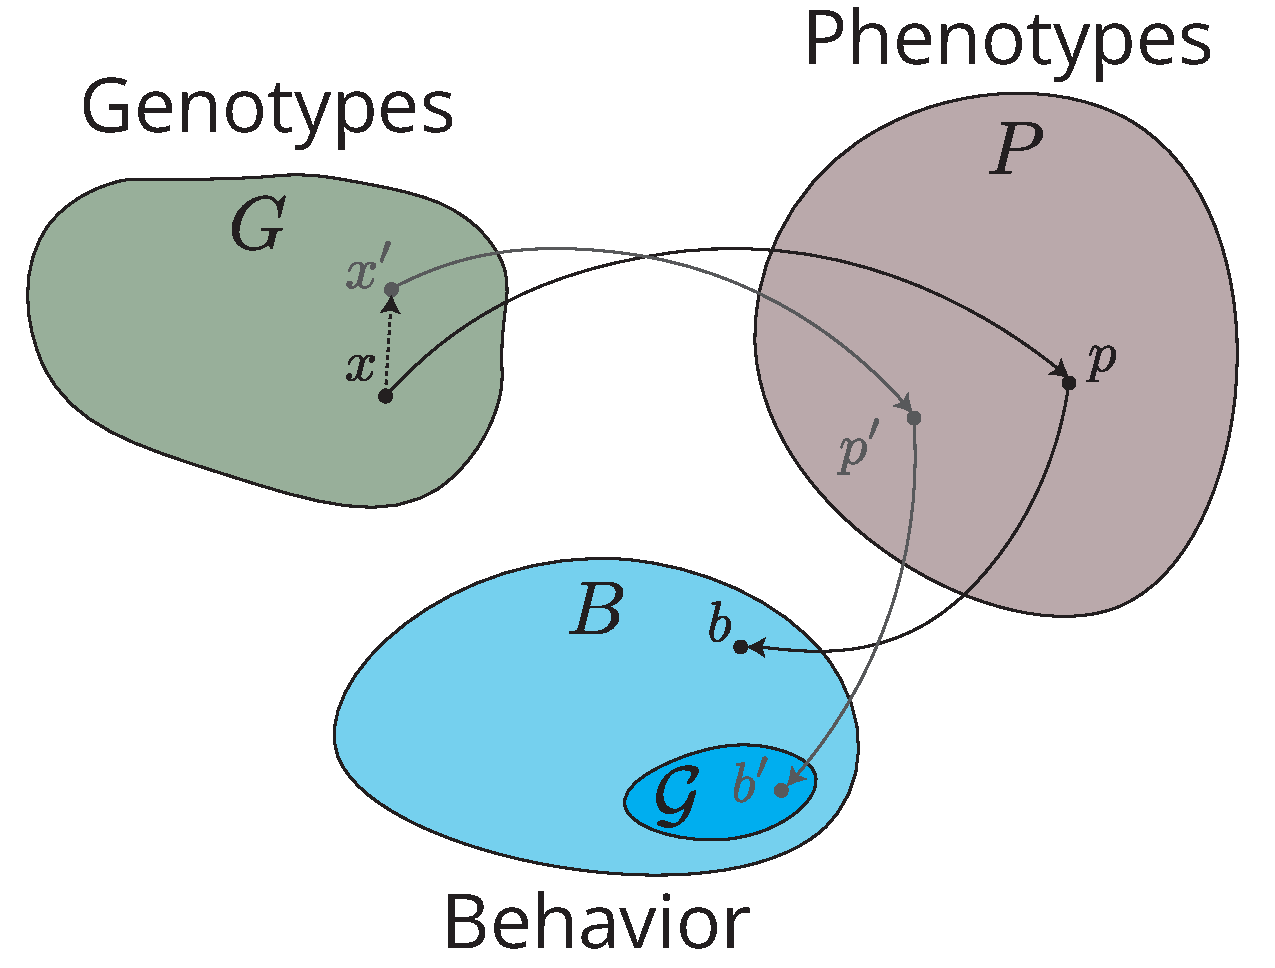
\includegraphics[width=.8\linewidth]{figures/evolutionary_diagram.pdf}
  \caption{Illustration of the general principle common to several evolutionary
    algorithms. There are three virtual spaces: ($G$) the genotype space where
    the candidate solutions are generated through some encoding. This is the
    space where the search process is happening. ($P$) the phenotype space,
    which corresponds to the decoded solution from a genotype $x$. It can be the
    policy of an agent, the rule of a \ac{CA}, etc. ($B$) the behavior space,
    which is the space from which candidate solutions are evaluated. The smaller
    subspace $\mathcal{G}$ is the goal space, corresponding to the set of
    behaviors that would be considered successful. A small perturbation in the
    genotype will have potentially large consequences on the behavior of the
    candidate solution.}
  \label{fig:evolutionary_diagram}
\end{figure}

\subsection{Genetic programming}
Many of the problems that machine learning, artificial intelligence are
attempting to solve require the discovery of a computer program that produces
some desired mapping between inputs and outputs. Solving the problems therefore
amounts to searching the space of computer programs in order to find a suitable
individual with high enough fitness
\parencite{langdonFoundationsGeneticProgramming2002,
  kozaGeneticProgrammingMeans1994, banzhafGeneticProgrammingIntroduction1998,
  ,bookerClassifierSystemsGenetic1989}.

In genetic programming, candidate solutions to a problem are encoded as
\emph{chromosomes}, that is a structured data representation that can be
modified incrementally. In practice it is often chosen to be a string of bits.
Every generation, a population of solutions is evaluated. The best solutions are
kept and combined to form the candidates for the next generation. Random
mutations may also be applied to introduce randomness in the search.

\subsection{Novelty search}
The idea behind \ac{NS} is to drive a search algorithm only by the novelty of
produced behavior \parencite{lehmanAbandoningObjectivesEvolution2011}. The most
counter-intuitive feature of this algorithm is that the actual objective of the
task is not taken into account at all during the search process. Generated
agents are evaluated solely on the novelty of their behavior. Despite this, it
appears to be at least as efficient as other search processes that are goal
focused, such as maze navigation and biped locomotion
\parencite{lehmanAbandoningObjectivesEvolution2011}, swarm robotics
\parencite{gomesEvolutionSwarmRobotics2013}, or neural network design
\parencite{risiEvolvingPlasticNeural2010}.

The principle of guiding search by novelty alone is closely related to the goal
this thesis, and especially with the challenge of parametrizing and searching
the space of available complex systems without using any explicit goal function.
The goal of \ac{NS} is to carry out search without a goal function, and we draw
inspiration from this algorithm throughout our work.

\begin{figure}[htbp]
  \centering
  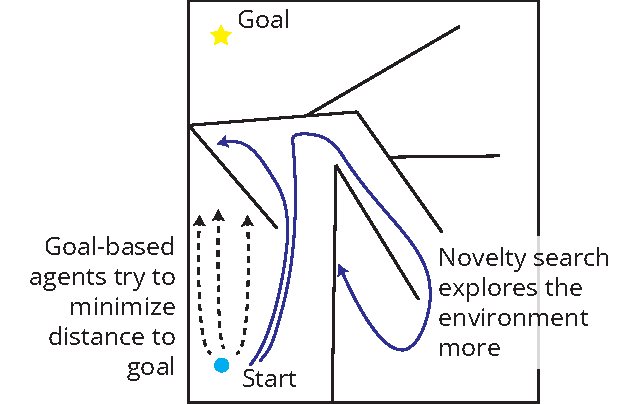
\includegraphics[width=.7\linewidth]{figures/novelty_search}
  \caption{Illustration of the advantage of \ac{NS} on a maze environment with
    deceptive dead-ends. Dotted trajectories illustrate the behavior of a
    goal-based search, which will start by minimizing the distance to the goal.
    Blue trajectories are from a novelty search algorithm exploring the space
    more efficiently. This type of maze environment was proposed by
    \textcite{lehmanAbandoningObjectivesEvolution2011}.}
\label{fig:novelty_search}
\end{figure}

This method has some limits, which are caused by a relative lack of theoretical
understanding of the effects of the parameters of \ac{NS}. The choice of
behavior descriptors for determining the novelty of agents is also not
straightforward. Several empirical studies have investigated the impact of a
range of parameters on the performance of \ac{NS}
\parencite{gomesDevisingEffectiveNovelty2015,
  kistemakerCriticalFactorsPerformance2011}, while other works have begun to
shed light on the theory \parencite{doncieuxNoveltySearchTheoretical2019}. In
practice \ac{NS} algorithms are expected to cover the exploration space well
\parencite{cullyQualityDiversityOptimization2017,pughQualityDiversityNew2016},
in some cases uniformly \parencite{gomesDevisingEffectiveNovelty2015}. \ac{NS}
algorithms are related to genetic algorithm since they maintain a population,
that is a set of individuals used to measure the novelty of current solutions.
There is also an archive of behavior of previous individuals to ensure that the
novelty is measured against all previously generated behaviors. There exists
multiple strategies for maintaining this archive
\parencite{gomesDevisingEffectiveNovelty2015}. Some use individuals whose
novelty was above a threshold when first evaluated
\parencite{lehmanAbandoningObjectivesEvolution2011}, the most novel individuals
of each generation \parencite{liapisConstrainedNoveltySearch2015}, random
individuals from the past generations
\parencite{lehmanEfficientlyEvolvingPrograms2010}, or none at all
\parencite{mouretEncouragingBehavioralDiversity2012}. An alternative to
explicitly measuring novelty in \ac{NS} is \emph{fitness sharing}. The goal of
fitness sharing is to encourage the diversity of a population by making them
share virtual ``resources'' \parencite{goldbergSimpleGeneticAlgorithms1987,
  hollandAdaptationNaturalArtificial1992}. A particular implementation of
\ac{NS} using this idea, with rewards physically spread out across the
environment was done by \textcite{herelEmergenceNoveltyEvolutionary2022}.

Typically, novelty search algorithms use one of a few types of maps from
genotypes to phenotypes, that is a map from the space of encoded solution to
agent and policy implementation
\parencite{mouretEncouragingBehavioralDiversity2012}. Some common ones are:

\begin{itemize}
  \item A \ac{RNN} (of type \cite{elmanFindingStructureTime1990} or
        \cite{jordanSerialOrderParallel1997}), for which the weights are
        directly searched. For input size $n_{i}$ output size $n_{o}$, and
        hidden size $n_{h}$, $n_{i}n_{h} + n_{h}n_{o} + n_{h}^{2}$ weights must
        be evolved.
  \item Neuro-evolution of augmenting topology (NEAT,
        \cite{stanleyEvolvingNeuralNetworks2002}), which is an encoding of both
        neural network weights and architectures that has a built-in mechanism
        to sustain diversity.
\end{itemize}


\section{Open-ended evolution\label{sec:open-ended-evolution-1}}
The field of Artificial Life research has worked to figure out what the
fundamental conditions for the emergence of living systems are, and how to
create a process that can display analogous levels of creativity and complexity
as natural evolution \parencite{eigenHypercycle1979,
  langtonArtificialLifeProceedings1989, dysonOriginsLife1999,
  stanleyWhyOpenEndednessMatters2019, packardOverviewOpenEndedEvolution2019,
  sorosOpenendednessLastGrand2017}. It build upon the data and understanding we
collected about the process of life, but abstracts from any specific living
process and attempts to integrate various approaches into one unified research
to extract the first principles of life. A major assumption underpinning this
research is that this natural evolution as a process can be implemented equally
well in different media \parencite{dennettDarwinDangerousIdea1996}.

A system that behaves like natural evolution, producing a seemingly endless
amount of novelty and complexity starting from elementary building blocks is
called \emph{open-ended}. The main challenge of \ac{OEE} research is there is
not a simple single test for the phenomenon, but instead different kinds of
open-ended evolution exist. Systems can exhibit more than one kind at a time. In
the report from a workshop on \ac{OEE} at York
\parencite{taylorOpenEndedEvolutionPerspectives2016}, the authors summarized the
different kinds of \ac{OEE}, which were further refined in a follow up work
\parencite{packardOverviewOpenEndedEvolution2019}. They are as follows:

\begin{enumerate}
  \item Interesting new kinds of entities and interactions
  \item Evolution of evolvability
  \item Major transitions
  \item Semantic evolution
\end{enumerate}

The first category describes the ability of a system to construct new entities
with different properties, behavior, or interactions with other entities. For
example, the Tierra simulation sees entities emerge that exploit the computing
power of others, acting as parasites \parencite{srayApproachSynthesisLife1991}.
The second type is related to how open-end evolution itself can be evolved
through the emergence of multiple ``stepping stones'' that enable higher level
evolutionary units to be used by individuals or through interactions
\parencite{patteeEvolvedOpenEndednessNot2019}.

\subsection{Defining open-endedness}

Several necessary conditions and requirements have been identified across the
\ac{OEE} literature, which form an overlapping set of potential research
directions for developing open-ended systems. We list a few of these conditions
here. First, \textcite{maleyFourStepsOpenended1999} identifies four requirements:

\begin{enumerate}
  \item An open-ended evolutionary system must demonstrate unbounded diversity
        during its growth phase.
  \item An open-ended evolutionary system must embody selection.
  \item An open-ended evolutionary system must exhibit continuing new adaptive
        activity.
  \item An open-ended evolutionary system must have an endogenous implementation
        of niches.
\end{enumerate}
Next, \textcite{sorosIdentifyingNecessaryConditions2014} identified four more necessary
conditions which are as follows

\begin{enumerate}
  \item A rule should be enforced that individuals must meet some minimal
        criterion (MC) before they can reproduce, and that criterion must be
        nontrivial.
  \item The evolution of new individuals should create novel opportunities for
        satisfying the MC.
  \item Decisions about how and where individuals interact with the world should
        be made by the individuals themselves.
  \item The potential size and complexity of the individuals' phenotypes should
        be (in principle) unbounded.
\end{enumerate}
Then, \textcite{taylorRequirementsOpenEndedEvolution2015} also stated five
requirements for an open-ended system:

\begin{enumerate}
  \item Robustly reproductive individuals.
  \item A medium allowing the possible existence of a practically unlimited
        diversity of individuals and interactions, at various levels of
        complexity.
  \item Individuals capable of producing more complex offspring.
  \item An evolutionary search space that typically offers mutational pathways
        from one viable individual to other viable (and potentially fitter )
        individuals.
  \item Drive for continued evolution.
\end{enumerate}
Taylor also states a more general condition that should be sufficient for
creating an open-ended system as ``evolutionary dynamics in which new,
surprising, and sometimes more complex organisms continue to appear''
\parencite{taylorRequirementsOpenEndedEvolution2015,
  taylorOpenEndedEvolutionPerspectives2016}.

All these conditions illustrate a major challenge of \ac{OEE} research: the lack
of clear definition or notion of what exact conditions make a system open-ended.
We seem to agree about what is not open-ended, but whenever a constraint or
requirement for \ac{OEE} is identified, subsequent evidence forces us to refine
them later. This is related to the problem of complexity, for which no single
definition exists \parencite{johnsonSimplyComplexityClear2009}.

A common process to produce systems that behave analogously to natural evolution
is to start from evolvable units or building blocks
\parencite{srayApproachSynthesisLife1991, simsEvolvingVirtualCreatures1994,
  ofriaAvidaSoftwarePlatform2004, yaegerComputationalGeneticsPhysiology1994,
  channonImprovingStillPassing2003, spectorDivisionBlocksOpenended2007,
  sorosIdentifyingNecessaryConditions2014}. The reason is that starting from
higher level primitive units whose emergence would be hard to characterize may
be easier and faster than starting from lower level components. Results obtained
from these systems are often surprising, since they bear some key resemblances
to natural evolutionary processes. For example we note the emergence of
parasitic entities within the Tierra simulation
\parencite{srayApproachSynthesisLife1991}. The process of emergence of these
building blocks from simple rules and components has also been investigated
significantly \parencite{bagleySpontaneousEmergenceMetabolism1991,
  huttonEvolvableSelfReproducingCells2007, flammEvolutionMetabolicNetworks2010,
  sayamaSeekingOpenendedEvolution2011}. It appears harder to bridge the gap and
create high level evolutionary-like processes and behaviors from elementary
rules and substrates.

\subsection{Open-endedness in cellular automata}
One class of system that has rich interactions between each of its components as
well as no predefined evolvable units or assumptions about individuality is the
\ac{CA}. One of the very first automata, Von Neumann's self-reproducing machine,
was designed with goals that align with open-ended evolution, which is to build
a machine with no central controller and limited local interaction that can
self-reproduce as a whole
\parencite{vonneumannTheorySelfreproducingAutomata1966,
  pesaventoImplementationNeumannSelfReproducing1995}. Later, other
self-replicating structures such as Langton's loop
\parencite{langtonSelfreproductionCellularAutomata1984} and evoloops
\parencite{sayamaNewStructurallyDissolvable1999,
  salzbergComplexGeneticEvolution2004} showed that more properties of open-ended
systems can be included in a \ac{CA}. A potential limitation of \acp{CA} is the
absence of notion of conservation of ``matter''. For example, the game of life
can start from a configuration with very few live cells and create many more at
no cost during its evolution. Some authors believe that this conservation
property is essential to the construction of an open-ended evolving system
\parencite{taylorChapterCreativityEvolution2002}.

\subsection{Artificial chemistries}
Most of the time, \acp{AC} are not trying to accurately model chemical processes
(as in \parencite{ostrovskyCellularAutomataPolymer2001} for example). Instead,
they build models of the dynamics of complex molecular processes that lead to
evolutionary behavior \parencite{dittrichArtificialChemistriesReview2001}. By
abstracting away from the natural molecular processes, \acp{AC} tries to uncover
fundamental conditions for the emergence of organization, self-maintenance, or
self-construction with basic building blocks. There are various approaches for
building these \aclp{AC}, of which we review a few here.

\paragraph{Rewriting systems.}
Rewriting systems are composed of entities or symbols that get modified
according to a set of syntactic rules. Patterns of symbols or entities are
replaced according to these rules.

\paragraph{Cellular automata.}
\Acfp{CA} can be see as a particular case of lattice molecular systems. For
example the autopoietic system introduced by
\textcite{varelaAutopoiesisOrganizationLiving1991} is a 2d square grid with
sites that be occupied by \emph{atoms} which is similar to a \ac{CA} with 4
states. Each of these states is analogous to a chemical component of the system:
($\emptyset$) empty site, (S) substrate, (K) catalyst and (L) monomer. Basic rules are
applied asynchronously and define how neighboring atoms interact with each
other. Remarkably, stable self-repairing cells arise spontaneously from these
basic rules. Their membrane is composed of a chain of monomers, which is
maintained by the substrate and catalyst reacting according to the rules. Some
key components of that model were investigated in other works, showing that they
are crucial for autopoeisis to be possible
\parencite{zelenySelforganizationLivingSystems1977,
  mcmullinRediscoveringComputationalAutopoiesis1997}.

\section{Computing with complex systems}\label{sec:comp-with-compl}

The problem of computing within complex systems is closely related to the
question of decentralized parallel computation in general, for which there exist
an abundant literature. Different paradigms exist for controlling and harvesting
the computations within complex systems. Several other names have been used for
closely related topics, such as organic computing
\parencite{muller-schloerOrganicComputingParadigm2011} which is the study of
systems with life-like properties such as self-organization or the ability to
adapt to a dynamically changing environment. Agent-based computing
\parencite{jenningsAgentBasedComputingPromise1999} focuses on computing systems
composed of several relatively simple autonomous agents. Amorphous computing
\parencite{abelsonAmorphousComputing2000,
  nagpalProgrammablePatternFormationScaleIndependence2008,
  nagpalProgrammableSelfassemblyUsing2002} is about making vast quantities of
individual computing elements work, and to ensure ``the cooperation of vast
numbers of unreliable parts interconnected in unknown, irregular, and
time-varying ways''.

\subsection{Computing in cellular automata}\label{sec:comp-cell-autom}

\Acfp{CA} are decentralized parallel systems with many identical components with
local connectivity. Because of these properties, they have the potential to
carry out robust, efficient computations. \ac{CA}-based computing machines could
recover from perturbations or carry out computations in stochastic environments.
Moreover, they are also interesting for modeling the behavior of natural complex
systems. For more details about \acp{CA}, see section
\ref{sec:cellular-automata-sec}.

\paragraph{Von Neumann's self-reproducing \ac{CA}}
The early developments of \acp{CA} were guided by Von Neumann's question ``What
kind of logical organization is sufficient for an automaton to be able to
reproduce itself?''. Additional constraints were added so that the problem does
not admit trivial solutions. For example, Von Neumann required that the
automaton in question be equivalent in power to a universal Turing machine while
having minimal complexity
\parencite{vonneumannTheorySelfreproducingAutomata1966}. The final model was an
intricate \ac{CA} composed of a tape containing the instructions to construct
the next automaton, and a construction unit which would progressively build that
new automaton cell by cell.

\paragraph{Universal Computation in Cellular Automata}
It is not difficult to see that a \ac{CA} can be capable of universal
computation. The basic approach is to show that it can simulate a Turing
machine, which we assume has an infinite tape. A \ac{CA} rule can be constructed
by reproducing all the steps of a Turing machine's behavior while adding a state
to each cell indicating wether it is active or not, and enforcing that only one
cell is active at a time. This turns the parallel \ac{CA} into a sequential
object that simulates a Turing machine. A similar construction was carried out
by \parencite{smithSimpleComputationUniversalCellular1971}, making a \ac{CA}
with one-to-one correspondence between its time steps and that of a target
Turing machine.

Another approach was used to show the universality of the game of life (see
details in section \ref{sec:game-life}). Instead of simulating a Turing machine,
basic logical functions are built from gliders (see figure \ref{fig:glider})
produced by a game of life structure called \emph{glider gun}. Two gliders that
collide within the simulation will either annihilate or keep moving depending on
the exact position in which they collide. This allows constructing NOT, AND and
OR gates. For example see figure \ref{fig:gol_not_gate} for a construction of a
NOT gate.

\begin{figure}[htbp]
  \centering
  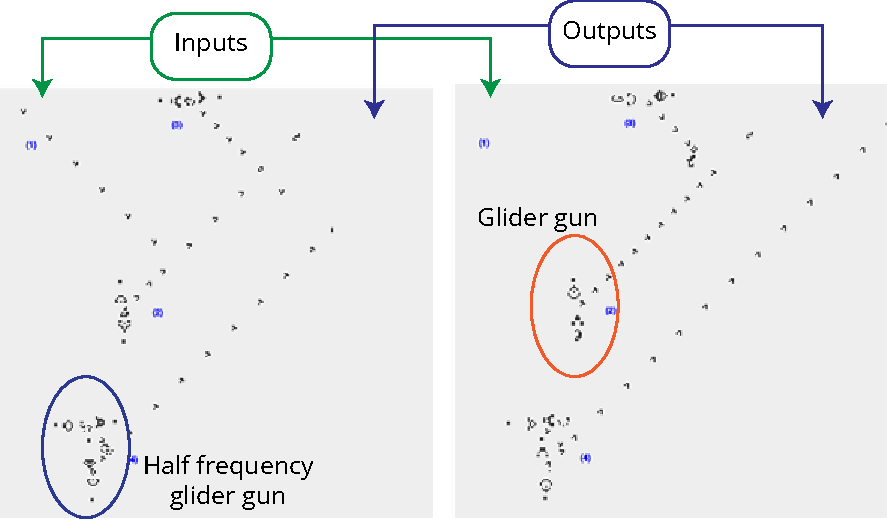
\includegraphics[width=.8\linewidth]{figures/gol_not_gate}
  \caption{Construction of a NOT gate in game of life. The left image represents
    an input equal to 1, while the second shows an input equal to 0. Output
    streams behave like a NOT gate. A glider gun and a modified half-frequency
    glider gun are highlighted. They are necessary to the construction of the
    gate. Images are adapted from a blog post
    \parencite{carliniDigitalLogicGates2020}.}
  \label{fig:gol_not_gate}
\end{figure}

Universal computation is an intriguing yet impractical property, and proving
that a system is a universal computers often has limited usability, but it
serves as a proof of principle that the studied system is theoretically as
powerful as any computer. In the case of the game of life, this was illustrated
by the implementation of the OTCA metapixel which is a tileable square cell
object that can be used to simulate another instance of game of life within the
game. It is important to note that such embedded computers and Turing machines
are often very slow and inefficient, and the game of life has brittle structures
which would be destroyed by the slightest perturbation, making these
construction unusable for anything else than demonstration.

\paragraph{Evolving cellular automata with genetic algorithms}
A major step forward from the clever but difficult hand-design of \acp{CA} rules
to perform computations is the use of learning algorithms to automatically
design those rules \parencite{mitchellEvolvingCellularAutomata1996}. Genetic
algorithms are a type of search method inspired by biological evolution
\parencite{bookerClassifierSystemsGenetic1989}. See section

Some early work was done by Norman Packard and colleagues
\parencite{packardAdaptationEdgeChaos1988,
  richardsExtractingCellularAutomaton1990}.
\textcite{richardsExtractingCellularAutomaton1990} use genetic algorithms to
learn the rules of a \ac{CA} to match experimental data for the patterns created
by the dendritic solidification of \ce{NH4Br}. In
\parencite{packardAdaptationEdgeChaos1988}, the author evolves \acp{CA} to
perform a specific computation, and observes that the evolution process tends to
select \acp{CA} with a $\lambda$ parameter close to the critical value observed
by Langton which corresponds to the edge of chaos (see section
\ref{sec:langtons-lambda} for details about the parameter). However, other
authors were unable to replicate it \parencite{mitchellRevisitingEdgeChaos1993}.
\textcite{kozaEvolutionSubsumptionUsing1992} applied genetic algorithms to
\acp{CA} to generate random numbers.

The problem of density classification was thoroughly explored since it fits the
\ac{CA} paradigm particularly well \parencite{mitchellRevisitingEdgeChaos1993,
  mitchellEvolvingCellularAutomata1994,
  crutchfieldEvolutionEmergentComputation1995, dasGeneticAlgorithmDiscovers1994,
  sipperCoevolvingNonuniformCellular1996, andreDiscoveryGeneticProgramming1996}.
The goal of this task is to have \ac{CA} decide the most abundant type of cell
in a binary initial state in one dimension. This task is trivial for a central
controller that can read the state of all the cells in the initial grid, but it
is much more complex for a decentralized systems like \ac{CA} with a small
radius of interaction with neighbors. The evolved \ac{CA} developed various
strategies to solve the task. Some are unsophisticated, such as expanding the 1s
or 0s, which does not work on all validation examples. We show one of the more
sophisticated solutions discovered by the genetic algorithm on figure
\ref{fig:particle_ca}.

\begin{figure}[htbp]
  \centering
  \begin{subfigure}[b]{.4\linewidth}
    \centering
    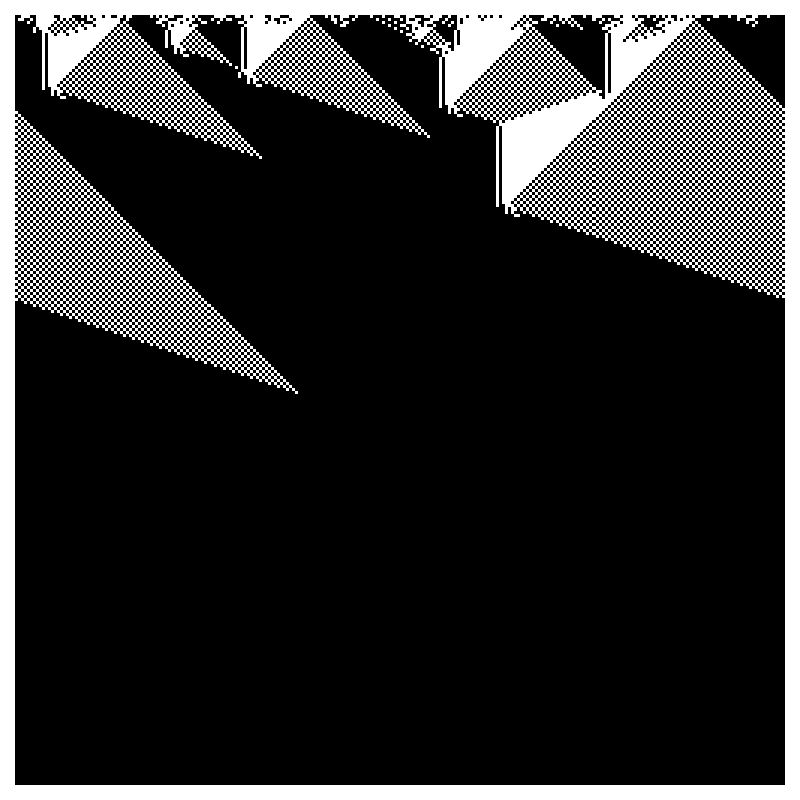
\includegraphics[width=\linewidth]{figures/particle_ca_full.png}
    \caption{Density $> 0.5$}
    \label{fig:particle_ca_full}
  \end{subfigure}
  \hspace{10pt}
  \begin{subfigure}[b]{.4\linewidth}
    \centering
    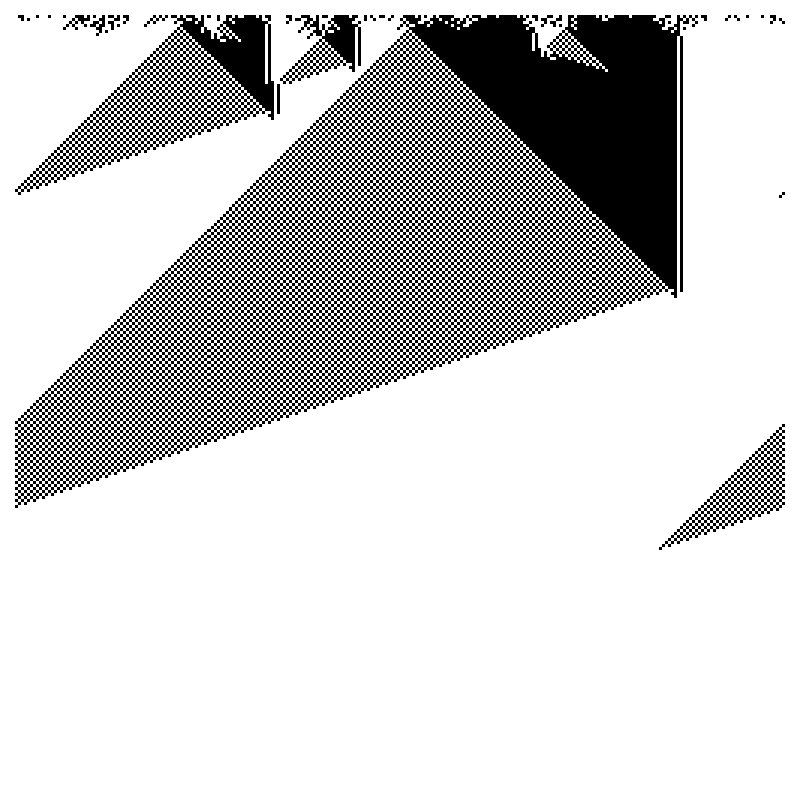
\includegraphics[width=\linewidth]{figures/particle_ca_empty.png}
    \caption{Density $< 0.5$}
    \label{fig:particle_ca_empty}
  \end{subfigure}
  \caption{The particule-based solution to the density classification problem
    \parencite{mitchellEvolvingCellularAutomata1996}. When the density is above
    0.5, the \ac{CA} quickly reaches a state with only black cells, whereas when
    the density is lower, it goes to a state with white cells only.}
  \label{fig:particle_ca}
\end{figure}


\paragraph{Reliable computation in cellular automata}
The problem of carrying out reliable computations in \acp{CA} is studied early
on in its history because of the potential of that model for real hardware
implementation. The first studies used probabilistic approaches for solving the
error detection and correction problems of automata --- which includes other
models than \acp{CA} \parencite{neumannProbabilisticLogicsSynthesis1956,
  winogradReliableComputationPresence1963,
  ,tsertsvadzeStochasticAutomataProblem1964,
  ,haraoConsiderationCellularAutomata1973}. Other methods make use of the
special structure of \ac{CA}, but rely on strong assumptions about the
likelihood of errors \parencite{haraoFaultTolerantCellular1975,
  nishioFaultTolerantCellular1975}. Peter Gács has shown how to construct a 1-d
CA which can perform arbitrarily large reliable computations, with each cell an
error with a positive probability
\parencite{gacsReliableComputationCellular1986}. The fault model he describes is
important from the point of view of ergodic theory because Gács’ result
invalidates the ``positive probability conjecture'' in statistical physics,
which states that all one dimensional infinite particle system with positive
transition probabilities is ergodic. For more recent work on fault-tolerance by
Gács, see \parencite{gacsReliableCellularAutomata2001}.

\paragraph{Neural cellular automata\label{sec:neur-cell-autom}}
The principle of \ac{NCA} is based on the analogy between \acp{CA} and two types
of neural networks: \acp{RNN} and \acp{CNN} (see Section
\ref{sec:cell-autom-rnns} for more details about the analogy). Once this link is
established, \ac{NCA} can be manipulated like neural networks, using automatic
differentiation, backpropagation and optimization algorithms to make these
models learn some target task. A first example used this neural network
representation to learn a \ac{NCA} version of existing \ac{CA} rules from
recorded examples of their evolution
\parencite{gilpinCellularAutomataConvolutional2018}. The structure of the
training process and final error of the resulting model is used by the author as
a tool to understand the complexity and properties of the original \ac{CA}.

\acp{NCA} were also used to learn to produce stable self-repairing patterns that
resemble a target image \parencite{mordvintsevGrowingNeuralCellular2020}. The
training process is structured in such a way that the \ac{NCA} needs to learn to
maintain the pattern stable across time and space, but also recover form random
perturbations that are introduced randomly. This results in an interesting demo,
where a pattern is generated and maintained in real time by a \ac{NCA} while a
user can directly apply
perturbations\footnote{\url{https://distill.pub/2020/growing-ca/}}.

\begin{figure}[htbp]
  \centering
  \begin{subfigure}[t]{.49\linewidth}
    \centering
    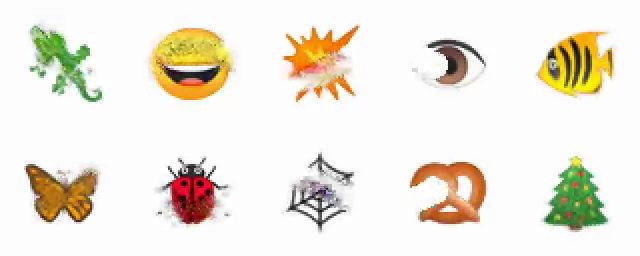
\includegraphics[width=\linewidth]{figures/nca_perturb.png}
    \caption{Perturbed patterns}
    \label{fig:nca_perturb}
  \end{subfigure}
  \begin{subfigure}[t]{.49\linewidth}
    \centering
    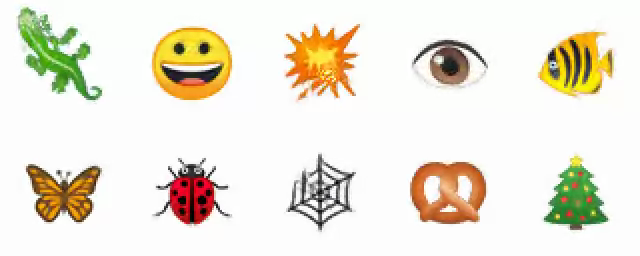
\includegraphics[width=\linewidth]{figures/nca_recover.png}
    \caption{Recovered patterns after a few hundred \ac{NCA} steps.}
    \label{fig:nca_recover}
  \end{subfigure}
  \caption[Resistance of patterns]{Resistance of patterns to perturbations with
    \acp{NCA}. \ac{NCA} can robustly maintain patterns, even under relatively
    strong perturbations (~10-20\% of the pattern's size). This image was
    generated with an online notebook based on code from Alexander
    Mordvintsev\footnotemark.}
  \label{fig:nca}
\end{figure}
\footnotetext{\url{https://colab.research.google.com/github/google-research/self-organising-systems/blob/master/notebooks/growing_ca.ipynb}}

The same authors also used \ac{NCA} to learn to classify digits from the MNIST
database of handwritten digits
\parencite{randazzoSelfclassifyingMNISTDigits2020}. The particularity of this
model is its ability to perform the classification in a decentralized way, by
having the \ac{NCA} change the color of the digits directly in the \ac{CA} grid.
Cells can only communicate with their direct neighbors, so the model has to
reach a consensus by propagating information across the grid. This is done in
parallel, so multiple digits can be classified simultaneously through this
progressive consensus
process\footnote{\url{https://distill.pub/2020/selforg/mnist/}}.
Another work used the same model to learn to continuously generate images with
the same texture as a target \parencite{niklassonSelfOrganisingTextures2021}.
Again, an advantage of this method is the ability to recover from perturbations.

\begin{figure}[htbp]
  \centering
  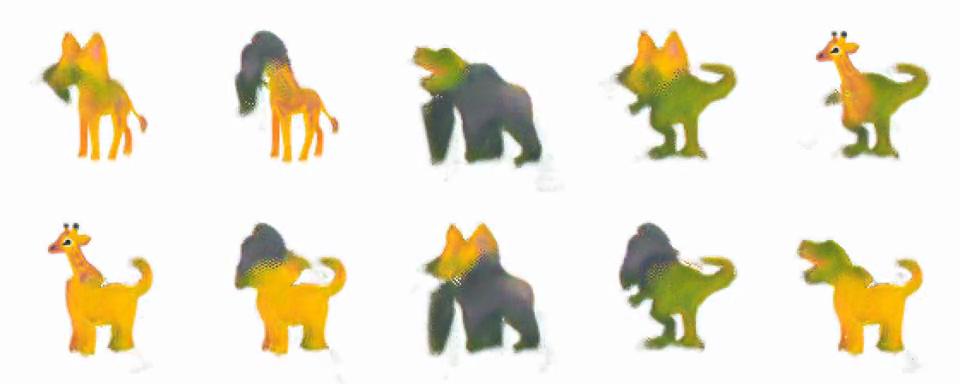
\includegraphics[width=.8\linewidth]{figures/nca_hybrids.png}
  \caption{Examples of stable hybrids obtained with \acp{NCA} trained with the
    method of \parencite{cisnerosOpenendedCreationHybrid2021}.}
  \label{fig:nca_hybrid}
\end{figure}


We used \ac{NCA} as part of our submission to the Minecraft open-endedness
challenge 2021\footnote{\url{https://evocraft.life/}}, a competition organized
at the Gecco 2021 conference competition
track\footnote{\url{https://gecco-2021.sigevo.org/Competitions}}
\parencite{cisnerosOpenendedCreationHybrid2021}. The goal was to build an
open-ended system within the computer game Minecraft. This means building a
systems that fullfils the following requirements:

\begin{itemize}
  \item Divergence: Open-ended algorithms are not expected to slow down or
        converge but rather keep expanding and generating more complex outputs
        over time.

  \item Diversity: Does the algorithm produce entities with strong phenotypic
        diversity?

  \item Complexity: Can the algorithm produce complex entities or entities
        interactions that give rise to complex systems? Are hierarchical and
        modular structures present?

  \item Ecological interactions: Do the created entities interact with each
        other?

  \item Life-Like properties: Inspiration may be taken from other attributes of
        living systems.
\end{itemize}

In each of the examples in figure \ref{fig:nca}, a separate \ac{CA} was trained
on a pattern starting from a single black pixel. We extend this by training a
single \ac{NCA} on multiple patterns from different seeds. Instead of a single
black cell, a small number of black cells are arranged into simple shapes We
call these patterns \emph{seeds}. \ac{NCA} have a lot of parameters. This
allowed us to learn more than one pattern (or larger patterns) without adding
parameters in the architecture. The resulting patterns are of slightly lower
quality but still stable under perturbations and able to grow.

We turned the process of combining seed patterns into a “game” by allowing user
interaction with the evolving CA through Minecraft. Our system is not open-ended
by itself, but needs human interaction to play with the shapes and seed
patterns. This is in the spirit of open-ended games like Picbreeder
\parencite{secretanPicbreederCaseStudy2011, woolleyDeleteriousEffectsPriori2011}
where players choose which generated patterns to mutate or evolve from. The
algorithms can generate endless novelty with the help of human interactions that
provide the missing step to make the system potentially open-ended.

\subsection{Amorphous computing}
The goal of amorphous computing is to study and define the problem of computing
with multiple interconnected components that are unreliable, irregular,
time-varying and with limited computational capacity
\parencite{abelsonAmorphousComputing2000}. The motivation for this research is
the development of biological substrates that can compute, function as sensors
and actuators, and robustly self-organize to compute with little cost. Precise
manufacturing of chemical or biological substrate with the ability to
communicate locally through chemical or physical interactions is within reach,
making the perspective of using them as computing vessels particularly
attractive. We can embed millions of chips with sensors
\parencite{abelsonAmorphousComputing2000} or program biological cells to serve
as logic gates \parencite{weissProgrammingBiologicalCells1998,
  weissVivoDigitalCircuits2002} while relying on cheaper, decentralized parts
\parencite{buteraProgrammingPaintableComputer2002}.

\begin{figure}[htbp]
  \centering
  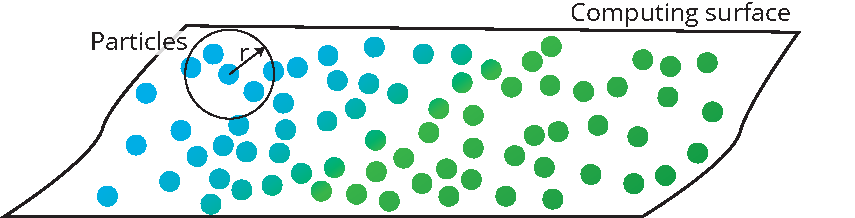
\includegraphics[width=.8\linewidth]{figures/amorphous_computing}
  \caption{An example of amorphous computing on a surface. Multiple computing
    particles are arranged randomly. A wave (represented by the color of the
    cells) propagates within the medium. They can communicate with neighbors
    within a radius $r$.}
  \label{fig:amorphous_computing}
\end{figure}

In an amorphous computing systems, a medium is composed of ``computational
particles'' spread on a surface or mixed in a volume. The particles have a
limited computing power, with no knowledge of their position or orientation. The
particles can communicate with neighbors via some specified mechanism, which may
be analogous to biological ones. There are two main components to this research
\begin{description}
  \item[Synthetic biology.] The design of a substrate from chemical processes or
        genetically engineered biological cells
        \parencite{weissVivoDigitalCircuits2002}. It should behave correctly and
        follow pre-defined rules.
  \item[Computing paradigm.] How to program the individual agents to follow a
        global predefined goal?
        \parencite{nagpalProgrammableSelfassemblyConstructing2001}
\end{description}


The growing point language (GPL) is an example of programming language that
enables programmers to specify complex patterns for computational particles,
which are internally represented in the particles as state machines
\parencite{cooreBotanicalComputingDevelopmental1999}.

\textcite{nagpalProgrammableSelfassemblyUsing2002} develops another programming
language, inspired from biological cell differentiation
\parencite{lawrenceMakingFlyGenetics1992,
  wolpertPositionalInformationSpatial1969}, that can compile to individual agent
programs to follow some global specification.

\chapter{Measuring complexity in evolving complex systems}
\label{cha:meas-compl-evolv}

  In this paper we propose an approach for measuring growth of complexity of
  emerging patterns in complex systems such as cellular automata. We discuss
  several ways how a metric for measuring the complexity growth can be defined.
  This includes approaches based on compression algorithms and artificial neural
  networks. We believe such a metric can be useful for designing systems that
  could exhibit open-ended evolution, which itself might be a prerequisite for
  development of general artificial intelligence. We conduct experiments on 1D
  and 2D grid worlds and demonstrate that using the proposed metric we can
  automatically construct computational models with emerging properties similar
  to those found in the Conway's Game of Life, as well as many other emergent
  phenomena. Interestingly, some of the patterns we observe resemble forms of
  artificial life. Our metric of structural complexity growth can be applied to
  a wide range of complex systems, as it is not limited to cellular automata.

\section{Introduction}
Recent advances in machine learning and deep learning have had successes at
reproducing some very complex feats traditionally thought to be only achievable
by living beings. However, making these systems adaptable and capable of
developing and evolving on their own remains a challenge that might be crucial
for eventually developing AI with general learning capabilities (for example as
is further discussed in \cite{mikolov2016roadmap}). Building systems that mimic
some key aspects of the behavior of existing intelligent organisms (such as the
ability to evolve, improve, adapt, etc.) might represent a promising path.
Intelligent organisms --- e.g., human beings but also most living organisms if
we consider a broad definition of intelligence --- are a form of spontaneously
occurring, ever evolving complex systems that exhibit these kinds of properties
\cite{booker_perspectives_2004}. The ability to sustain open-ended evolution
appears to be a requirement in order to enable emergence of arbitrarily complex
adaptive systems.

Although a rigorous attempt at defining intelligence or life is beyond the scope
of this paper, we assume that a system we might identify as evolving, with the
potential of developing intelligence, should have the property of
self-preservation and the ability to grow in complexity over time. These
properties can be observed in living organisms \cite{booker_perspectives_2004}
and should also be a part of computational models that aim to mimic them.

To recognize self-preservation and growth in complexity, one should be able to
detect emerging macro-structures composed of smaller elementary components. For
the purpose of obtaining computational models that grow in complexity over time,
one should also be able to determine the amount of complexity these systems
contain. We propose and discuss in this paper several ways of estimating the
complexity and detecting the presence of emerging and stable patterns in complex
systems such as cellular automata. We show that such metrics are useful when
searching the space of cellular automata with the objective of finding those
that seem to evolve in time.

\section{Related work}

\subsection{Artificial life and open-ended evolution}

Several works have attempted to artificially create open-ended evolution. A
non-exhaustive list of some well known systems include Tierra
\cite{s_ray_approach_1991}, Sims \cite{sims_evolving_1994}, Avida
\cite{ofria_avida:_2004}, Polyworld \cite{yaeger_computational_1994}, Geb
\cite{channon_improving_2003}, Division Blocks \cite{spector_division_2007} and
Chromaria \cite{soros_identifying_2014}. Designs focusing on an objective, and
making use of reinforcement learning methods to drive evolution are also being
studied, e.g. in \cite{pathak_learning_2019}. Most of these simulated ``worlds''
have had some success in reproducing key aspects of evolving artificial life,
enabling the emergence of complex behavior from simple organisms. However, they
still work within constrained simulated environments and usually consider
organisms composed of elementary building blocks, while they don't work outside
of this usually very constrained framework. Divergent and creative evolutionary
process could be happening at a much lower conceptual level with fewer
assumptions. For this reason, we consider cellular automata in the rest of the
paper because they rely on a very few assumptions while offering a very large
expressive power and a potentially wide range of behaviors that can be
discovered. However, the metrics defined in this paper have the potential to be
applied to other types of complex systems as discussed in
Section~\ref{sec:conclusion}.

\subsection{Cellular automata}

Cellular automata are very simple systems, usually defined in one or two
dimensions, composed of cells that can be in a set of states. The cells are
updated in discrete time steps using a transition table that defines the next
state of a cell given the states of its neighbors.
They were originally proposed by Stanislaw Ulam and studied by Von Neumann
\cite{von_neumann_theory_1966}, who was interested in designing a computational
system that can self-reproduce itself in a non-trivial way. The trivial
self-reproducing patterns were then those that do not have potential to evolve,
for example the growth of crystals.

Stephen Wolfram later took a more bottom up approach, beginning with the study
of the simple 1D binary cellular automata (CA), and identifying four qualitative
classes of cellular automaton behavior \cite{wolfram_universality_1984}:
\begin{description}
\item[Class 1]  evolves to a homogeneous state.
\item[Class 2]  evolves to simple periodic patterns.
\item[Class 3]  yields aperiodic disordered patterns.
\item[Class 4]  yields complex aperiodic and localized structures, including
  propagating structures.
\end{description}
Wolfram and his colleagues also studied 2D CA using tools from information
theory and dynamical systems theory, describing the global properties of
these systems in terms of entropies and
Lyapunov exponents \cite{packard_two-dimensional_1985}.

Christopher Langton and colleagues also studied CA dynamics
\cite{li_transition_1990} --- e.g. using the $\lambda$ parameter
\cite{langton_computation_1990} --- and designed a self-replicating pattern much
simpler than Von Neumann's \cite{langton_self-reproduction_1984}, now known as
Langton's loops. The main issues with his system and Von Neumann's universal
replicator is the fact that they are very fragile and based on a large amount of
human design. As a consequence, although they do self-replicate, they cannot
increase in complexity and are not robust to perturbations or unexpected
interactions with the environment.

A genetic algorithm-based search for spontaneously occurring self-replicating
patterns in 2D cellular automata with several states was undertaken in
\cite{bilotta_artificial_2011} using entropy measures of the frequency
distribution of $3\times 3$ patterns.

\subsection{Compression and complexity}
Compression has often been used as a measure of complexity. Lempel and Ziv have
introduced in \cite{lempel_complexity_1976} the now widespread Lempel-Ziv (LZ)
algorithm as a method for measuring the complexity of a sequence. By
constructing back-references to previous parts of a string, the LZ algorithm is
capable of taking advantage of duplicate patterns in the input to reduce its
size. The DEFLATE algorithm that we use in the following section combines LZ
with Huffman coding for efficient representation of the symbols obtained after
the first step. It is one of the most widespread compression algorithms and is
for instance used in gzip and PNG file compression standards.

The PAQ compression algorithm series \cite{mahoney_fast_2000} is an ensemble of
compression algorithms initially developed by Matt Mahoney with state of the art
compression ratio on several compression benchmarks. Better compression of an
input means a better approximation of the minimum description length and
implicit understanding of more of the underlying patterns in input data. The
usefulness of a better compressor is that it can detect much more complex and
intricate patterns that aren't simple repetitions of previous patterns.

In \cite{zenil_compression-based_2010}, H. Zenil investigates the effects of a
compression-based metric to classify cellular automata and observes that it
results in a partitioning of the space of 1D CA into several clusters that match
Wolfram's classes of automata. He also used this approach on the output of
simple Turing machines and some 1D automata with more than two states and larger
neighborhoods. Extensions of this work include asymptotic sensitivity analysis
of the compressed length for input configurations of growing complexity, as
introduced in \cite{zenil_asymptotic_2013, zenil_what_2014}.

Additionally, image decompression time as an approximation of Bennet's logical
depth \cite{bennett_logical_1995, zenil_image_2012} and the output distribution
of simple Turing machines combined with block decomposition of CA to approximate
their algorithmic complexity have also been investigated
\cite{zenil_two-dimensional_2015, soler-toscano_calculating_2014}. However, the
possible extent to which such measures of complexity could be applied to more
complex automata and other complex systems has not yet been extensively studied.
For a review of several measures of complexity and their applications, see
\cite{grassberger_randomness_1989}.

\section{Compression-based metric}\label{sec:compr-based-metr}

A cellular automaton of size $n$ in 1D can be represented at time $t$ by its
grid-state $S^{(t)} = \{c_1^{(t)}, ..., c_n^{(t)}\}$ where each $c_i$ (also
called a cell) can take one of $k$ possible values (representing the possible
states), and a transition rule $\phi$. The transition rule is defined with
respect to a neighborhood radius $r$ with the mapping $\phi(c^{(t)}_{i-r}, ...,
c^{(t)}_i ..., c^{(t)}_{i+r} ) = c^{(t+1)}_i$ that maps $\{1, ..., k\}^{2r+1}$
to $\{1, ..., k\}$. The quantity $2r + 1$ corresponds to the number of
cells taken into account for computing the next state of a cell, namely that
cell itself and $r$ neighboring cells in both directions.

Simulating a CA amounts to the recursive application of this mapping $\phi$ to
an initial state $S^{(0)} = \{c_1^{(0)}, ..., c_n^{(0)}\}$.

In the rest of the paper, we consider cyclic boundary conditions for the
automata, meaning that the indices $i-r, ..., i+r$ above are taken modulo $n$
the size of the automaton in 1D.  Boundary conditions can have some
effect on a CA's evolution, but cyclic boundaries have been empirically
observed to have limited effect on the complexity of automata in 1D
\cite{luvalle_effects_2019}.

The definition given in the equation above can be extended to higher dimensional
automata by modifying the neighborhood and the definition of $\phi$. A 2D
neighborhood of radius 1 can be defined as the 3 by 3 square around the center
cell --- also called the Moore neighborhood --- or by only considering the four
immediate horizontal and vertical neighbors of the center cell --- the Von
Neumann neighborhood.

Elementary cellular automata (ECA) are 1D CA with $k = 2$ and $r = 1$. There are
$2^3$ elements in $\{1, ..., k\}^{2r+1}$ and $2^{2^3} = 256$ possible different
set transition rules that are often compactly represented as a binary string
with 8 bits. The relatively low number of rules of this type makes it possible
to appreciate the performance of a metric and compare it with others.

We define the compressed length $C$ of a 1D cellular automaton at time $t$ as
\begin{align}
  \textstyle
  C(S^{T}) = \text{length}\left(\texttt{comp}(c_1\ ||\ c_2\ ||\ ...\ c_n)\right)
\end{align}

where $||$ denotes the string concatenation operator and the cells $c_i$ are
implicitly converted into string characters (with one symbol per unique state).
\texttt{comp} is a compression algorithm that takes a string as input and
outputs a compressed string, and length is the operator that returns the length
of an input string.

Similarly to \cite{kowaliw_measures_2008, zenil_compression-based_2010}, we use
zlib’s C implementation of DEFLATE to compress the final state of the automaton.
If we apply the above metric to the 256 ECA run for 512 timesteps and
initialized with one activated cell in the middle, we obtain the plot of
Figure~\ref{subfig:comp_scores}. This example is re-used in the paper as a way
to easily visualize and check that the defined complexity measures are coherent
with one another. The colors on Figure~\ref{subfig:comp_scores} were obtained
with a KMeans clustering algorithm applied on the compressed length of the
automata states.

\begin{figure}[tbp]
  \centering \subfloat[6 highest scoring automata. Only the first 30 timesteps
  are shown for readability.]{
    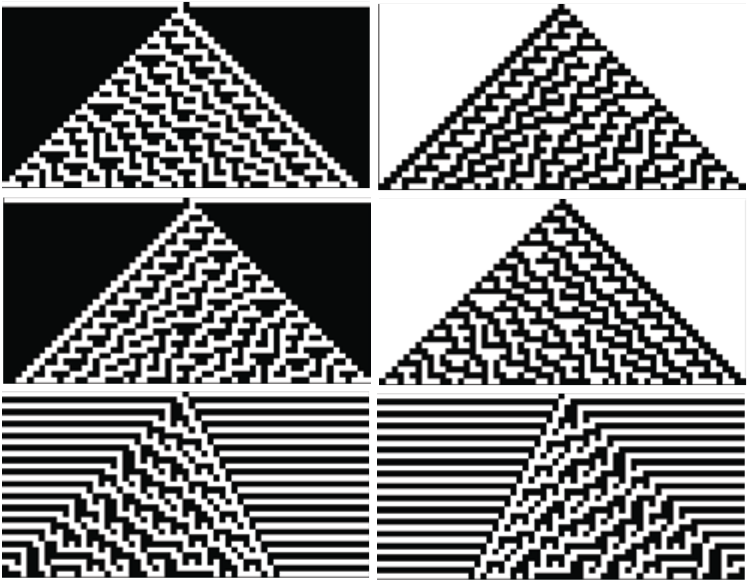
\includegraphics[width=.42\linewidth]{figures/complex_eca}
    \label{subfig:highest_6}
  }
  \hfil
  \subfloat[All 256 compressed length scores]{
    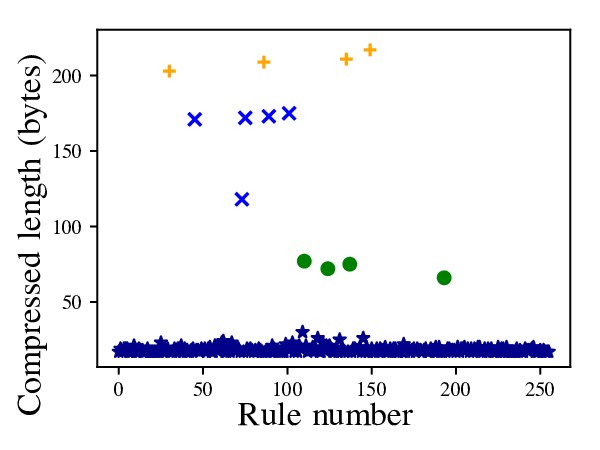
\includegraphics[width=.42\linewidth]{figures/one}
    \label{subfig:comp_scores}
  }
  \caption{Compression-based metric on 1D ECA. \ref{subfig:highest_6} represents
    the 1D ECA evolution with each line being the state of the automaton at a
    given timestep, starting from a single cell set to 1. Cells which are in
    state 1 are represented in black and cells in state 0 are represented in
    white. Time increases downwards. Figure~\ref{subfig:comp_scores} represents
    the compressed length of the 256 ECA rules, with different marker and colors
    corresponding to the obtained KMeans clusters.}
  \label{fig:comp_eca}
\end{figure}


As visible on Figure~\ref{subfig:comp_scores}, rules are clearly separated into
several clusters that turn out to match Wolfram’s classification of ECA. Class 3
behavior can be found at the top of the plot (highest compressed length, orange
and blue clusters), Class 1 and 2 are clearly separated at the bottom part (not
detailed here) and Class 4 rules (colored in green) lie in between the other
types of behavior. The 6 highest scoring rules are shown on
Figure~\ref{subfig:highest_6} and correspond to Class 3 behavior in Wolfram's
classification. Among the classes of behavior, some sub-clusters can be found
that correspond to similarly behaving rules.

Ultimately, the theoretical goal of using compression algorithms is to approach
the theoretical minimum description length of the input
\cite{grunwald_minimum_2007}. For very regular inputs, this length should be
relatively small and inversely for random inputs. However, gzip and PAQ are
crude approximations of the minimum description length, and may only approach it
in a given context. As an example, compressing text data (a task often performed
with gzip in practice) is much more efficient with a language model that can
assign a very low probability to non grammatically correct sentences. The
Kolmogorov complexity \cite{kolmogorov_three_1968} of a cellular automaton is
upper bounded by a value that is independent of the chosen rule, as it is
entirely determined by the transition table, the grid size, initial
configuration and number of steps.

\section{Predictor-based metric}

One obvious limit of using compression length as a proxy for complexity is the
fact that interesting systems mostly have intermediate compressed length.
Compressed length increases with the amount of disorder in the string being
compressed. Therefore, extreme lengths correspond either to systems that do not
increase in complexity on the lower end of the spectrum, or systems that produce
a maximal amount of disorder on the higher end. Neither of them have the
potential to create interesting behavior and increase in complexity.
Intermediate values of compressed length are also hard to interpret, since
average lengths might either correspond to interesting rules or slowly growing
disordered systems.

To cope with this limitation, one should also take into account the dynamics of
complexity, that is how the system builds on its complexity at a given time as
it keeps evolving, while retaining some of the structures it had acquired
earlier. Compression leverages the amount of repetitions in inputs to further
compress and this may also be used as an estimate of structure overlap, as
explained in the following section.

\subsection{Joint compression}\label{sec:joint-compression}

As a way to both measure the complexity and the amount of overlap between two
automata states apart in time, we define a joint compressed length metric for a
delay $\tau$ as
\begin{align}
  \textstyle C'\left(S^{(T + \tau)}, S^{(T)}\right) =
  C\left(S^{(T)}\ ||\ S^{(T + \tau)}\right)
\end{align}
where $||$ represents the concatenation operator. This quantity is simply the
compressed length of a pair of global states --- defined at the beginning of
\ref{sec:compr-based-metr}, represented by the letter $S$ --- at two timesteps
separated by a delay $\tau$. In 1D, concatenation means chaining the two string
representations before compressing, and in 2D we can chain two flattened
representations of the 2D grid. This introduces several issues which we discuss
in Section~\ref{sec:count-based-pred}.

To quantify the amount of overlap between the two global states, we can compute
the ratio of this joint compressed length with the sum of the two compressed
lengths $C(S^t)$ and $C(S^{t-\tau})$, thereby forming the joint compression
score
\begin{align}
  \textstyle \mu = \dfrac{C\left( S^t \right) +
  C\left( S^{t - \tau} \right)}{C'\left( S^t, S^{t - \tau} \right)}
\end{align}
defined for an automaton $S$, time $t$ and delay $\tau$.

This metric is based on the intuition that if patterns occur at step $T - \tau$
of the automaton's evolution and are still present at step $T$, the joint
compressed length will be lower than the sum of the two compressed length. The
idea is illustrated in Figure~\ref{fig:joint_schema}, where it is pointed out
that a stable moving structure (sometimes called \emph{glider} or
\emph{spaceships} in Game of Life) will yield lower joint compressed lengths.
This also applies to structures that self-replicate, grow from a stable seed or
maintain the presence of some sub-structures. Bigger structures yield a higher
compression gain.

\begin{figure}[htbp]
  \centering
  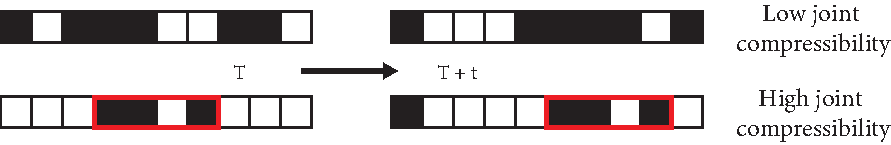
\includegraphics[width=.8\linewidth]{figures/joint_comp_1d}
  \caption{Joint compression method illustration. If a structure persists
    through time, this will decrease the joint compressed length compared to the
    sum of compressed lengths. A persistent structure is circled in red.}
  \label{fig:joint_schema}
\end{figure}

Joint compression alone is not sufficient since it only selects rules that
either behave like identity or shift input because they maximize the
conservation of structures through time --- as illustrated in
Figure~\ref{fig:high_eca_joint}. However, one may combine the joint compression
score with another complexity measure to only select rules that exhibit some
disorder, or growth in complexity --- as Figure~\ref{fig:high_eca_joint+comp}
shows (the condition here was a threshold on the difference of compressed length
between initial and final states).

\begin{figure}[htbp]
  \centering
  \subfloat[Highest joint compression score among the 256 ECA.]{
    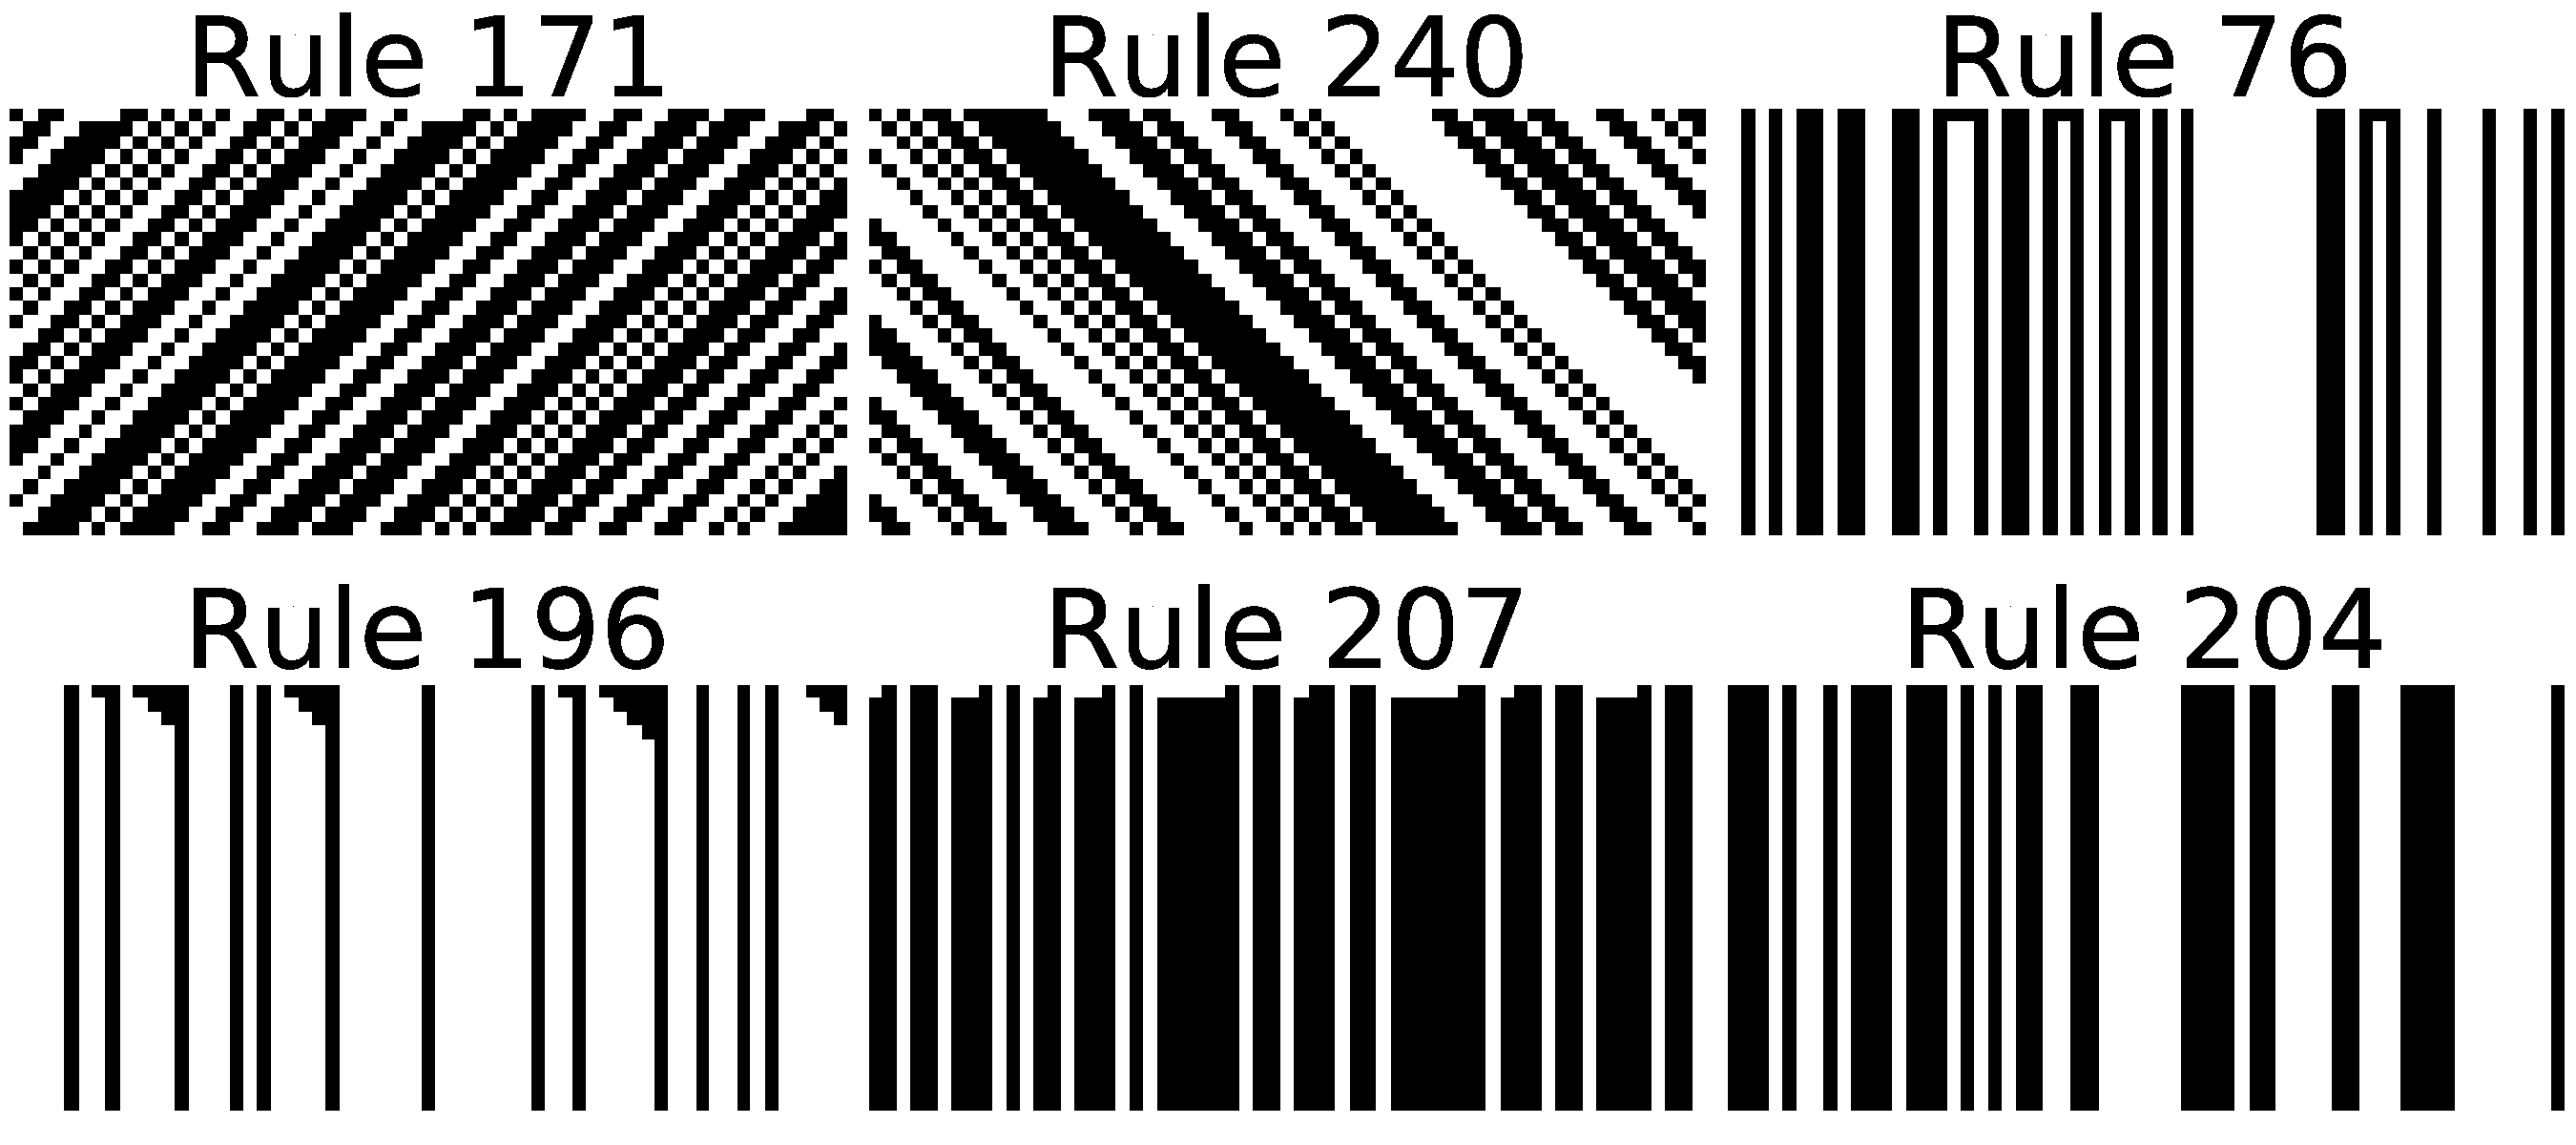
\includegraphics[width=.4\linewidth]{figures/high_eca_joint}
    \label{fig:high_eca_joint}
  }
  \hfil
  \subfloat[With condition on compressed length increase.]{
    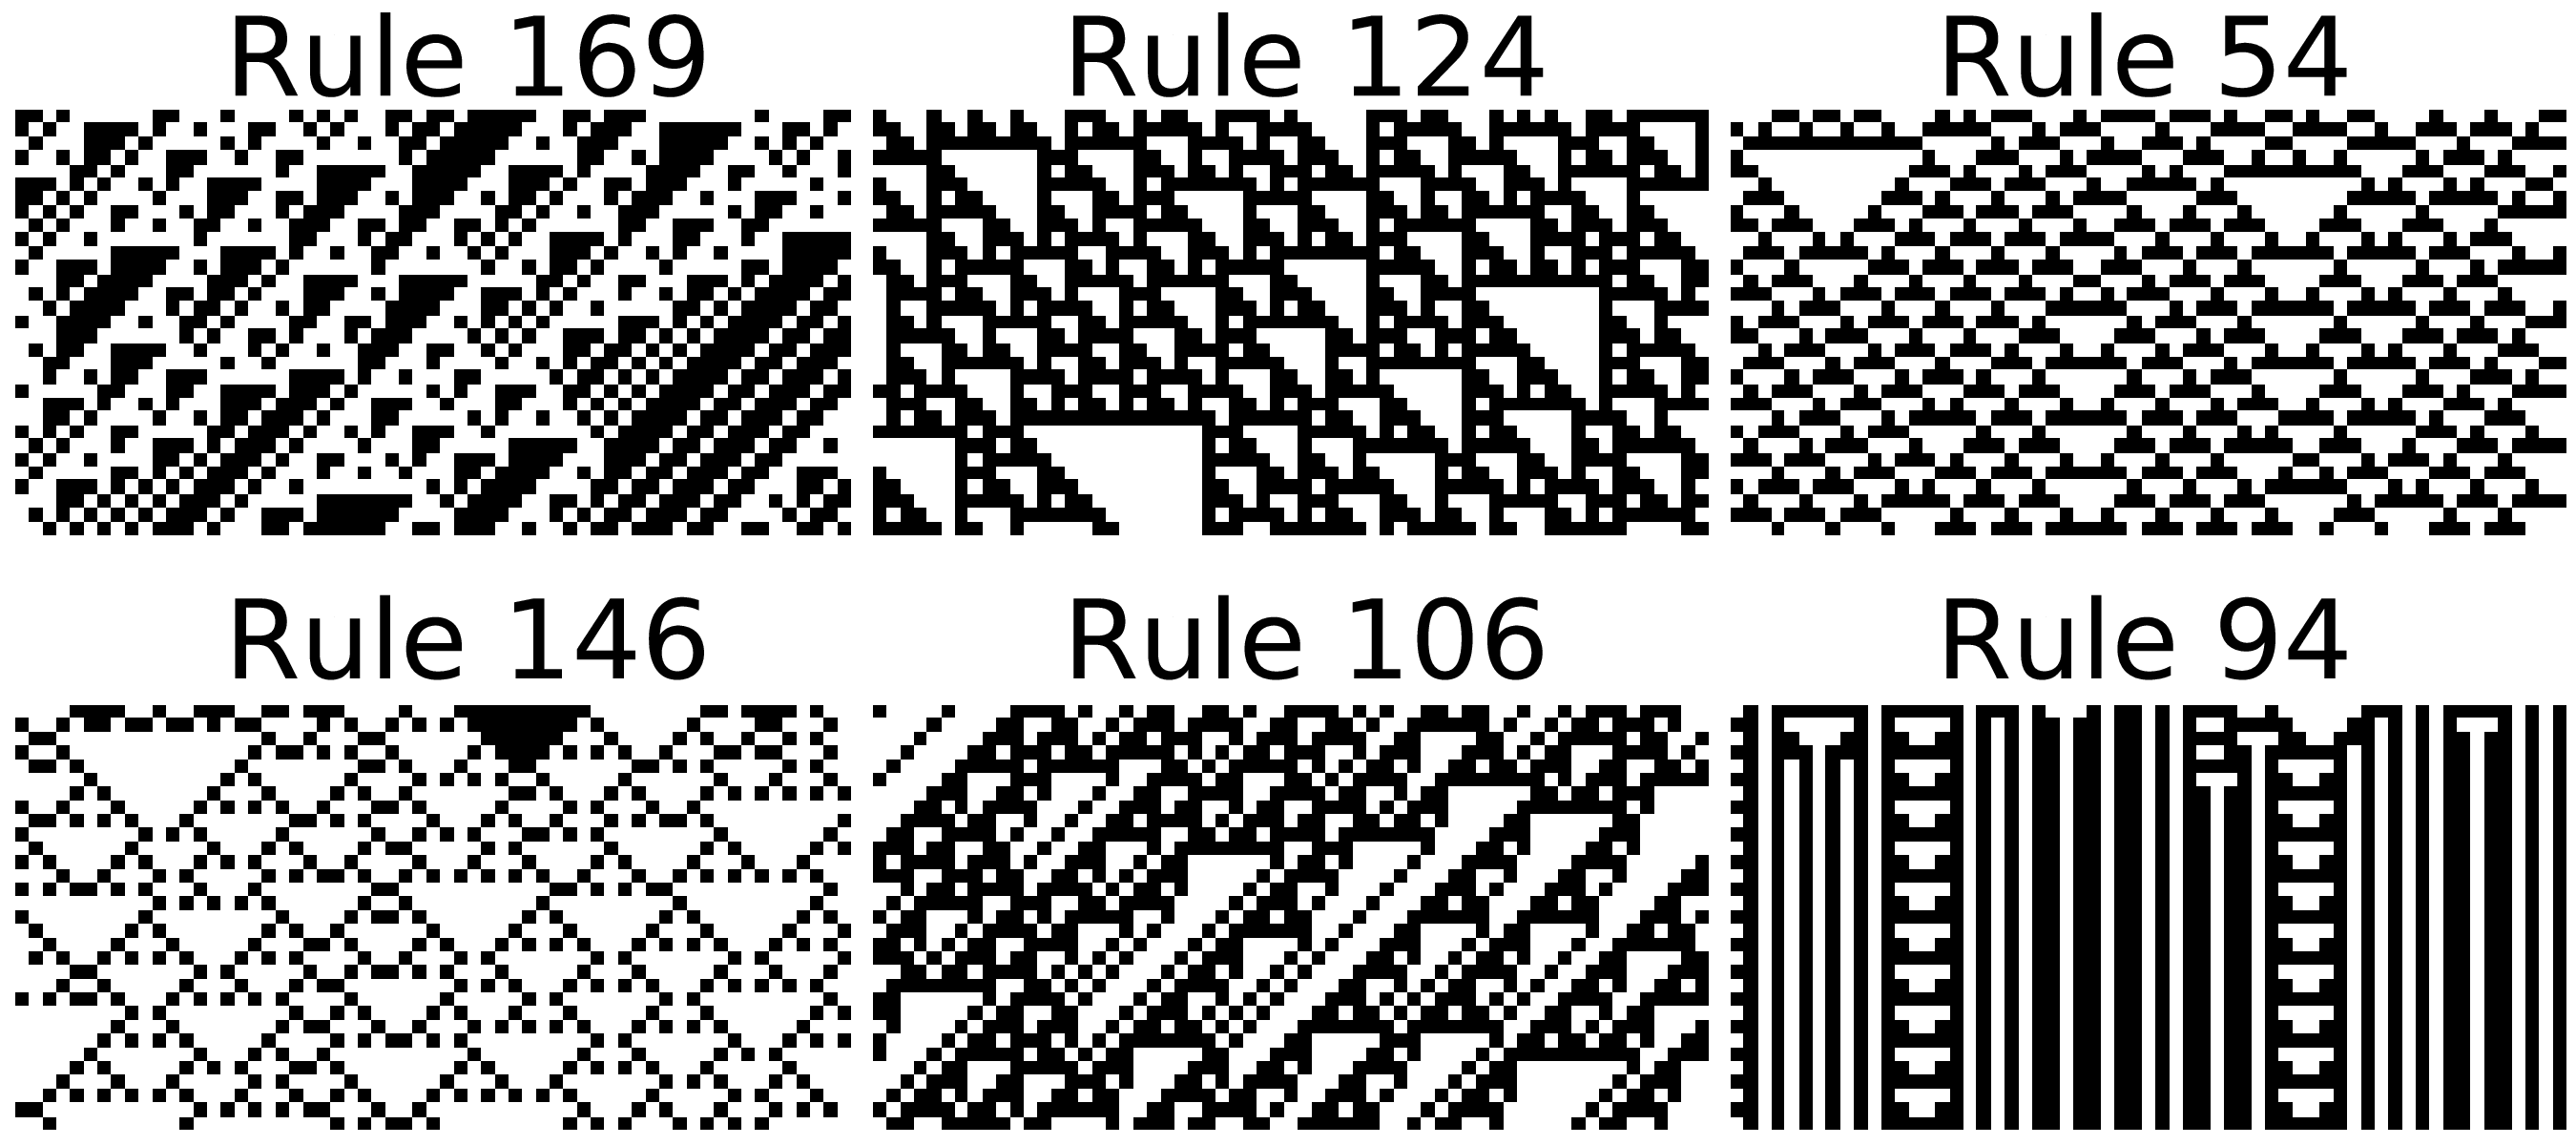
\includegraphics[width=.4\linewidth]{figures/high_eca_joint+comp}
    \label{fig:high_eca_joint+comp}
  }
  \caption{Comparison of the raw joint compression score and the addition of a
    complexity increase condition. The high overlap in structures is not enough
    to get interesting rules a shown in \ref{fig:high_eca_joint}, but the
    addition of a complexity threshold allows to retrieve rules with complex but
    still structured behavior, as shown in \ref{fig:high_eca_joint+comp}.
    Figures are from the same slice of 60 cells over 30 timesteps taken from
    larger automata with random initial states. The top row corresponds to $t =
    0$ and time increases downwards.}
  \label{fig:joint_highest}
\end{figure}

\subsection{Count-based predictor}\label{sec:count-based-pred}

A major issue with the joint compression metric is the fact that it is designed
to compress a linear stream of data. This is not ideal when considering higher
dimensional automata. Larger sets of transformations have to be
considered such as translations, rotations, flips, etc. Theoretically this
should not be a problem for a good enough linear compression algorithm, but
hardware and software limitations make it impractical to work with existing
algorithms on higher dimensional structures --- with e.g DEFLATE's upper limit
on dictionary size.

These higher dimensional automata might be better at generating complex
dynamics, and the large size of their rule spaces makes it a challenge to
explore. There has been at least one attempt to deal with these higher
dimensional systems \cite{zenil_two-dimensional_2015} that lacks the scalability
to work with large inputs.

An alternative to the linear compression-based method presented above would be
to use compressors optimized for n-dimensional data (e.g. PNG compression for 2D
automata) to take advantage of spatial correlation for compressing. However,
these compressors are rare for higher dimensional data, and are usually
optimized for one type of input --- e.g. images with PNG.

Another way to tackle the problem is to use a prediction based approach to
compression. Similarly to methods described in
\cite{schmidhuber_sequential_1996} and one of the first steps of the PAQ
compression algorithm \cite{mahoney_fast_2000}, we learn a statistical model of
input data to predict the content of a cell given its immediate predecessors.
For compression, this is often followed by an encoding step --- using Huffman or
arithmetic coding --- that encodes data which contains the least information
(least ``surprising'' data) with the most compact representation. This approach
can also be related to the texture synthesis method described in
\cite{efros_texture_1999}, where the authors learn a non parametric model to
predict the next pixel of a texture given a previously synthesized neighborhood.
Additionally, because we don't need the operation to be reversible as in regular
compression, it is not necessary to limit the prediction model to making
prediction with predecessors only.

For a global state $S = (c_{1}, ... c_i, ..., c_{n})$, the neighborhood of cell
$i$ with radius $r$, denoted $n_{r,i}$ is defined as the tuple $n_{r,i} =
(c_{i-r}, ... c_{i-1}, c_{i+1} ..., c_{i+r})$ --- without the middle cell. The
goal of this method is to estimate the conditional probability distribution $p(s
| n_r)$ of the middle states at timestep $T$ given a neighborhood of radius $r$.
Assuming cell states given their neighborhood can be modeled by mutually
independent random variables, the log-probability of global state $S^{(T)}$ is
written
\begin{align}
  \textstyle \log p(S^{(T)}) = \log \prod_{i=1}^N p(c_i | n_{r,i})  =
  \sum_{i=1}^N \log  p(c_i | n_{r,i})
\end{align}

If the automaton has a very ordered behavior, a model will predict with high
confidence the state of the middle cell given a particular neighborhood. On the
other hand, in the presence of maximal disorder, the middle cell will have an
equal probability of being in every state no matter the neighborhood. In the
latter case, a predictive model minimizing $-\log p(S^{(T)})$ would yield a high
negative log-probability.

A simple possible predictor for such purpose is a large lookup table that maps
all visited neighborhoods to a probability distribution over the states that the
middle cell can be in. State distributions for each neighborhood are obtained by
measuring the frequency of cell states given some observed neighborhoods. We
denote by $\Lambda$ this lookup table, defined for a window of radius $r$, which
maps all possible neighborhoods of size $2r + 1$ (ignoring the middle cell) to a
set of probabilities $p$ over the possible states $\{s_1, ..., s_n\}$, and $p$
can be written $[p_{s_1}, p_{s_2}, ... , p_{s_n}]$. $\Lambda$ is defined by
\begin{equation}
  \begin{aligned}
    \textstyle \Lambda :&& \{s_1, ..., s_n\}^{2r} &\to&& \Delta_n\\
    && n_{r,i} &\mapsto&& p
  \end{aligned}
\end{equation}
where $\Delta_n$ denotes the probability simplex in dimension $n$.

To measure the uncertainty of that predictor, we can compute the cross-entropy
loss between the data distribution it was trained on and its output. We compute
the log probability of the observed data given the model, or the quantity
\begin{align}
  \textstyle
  L = - \frac{1}{N}\sum_{i=1}^N \sum_{k=1}^n \mathds{1}_{\{ s_k \}}(c_i)
  \log\Lambda(n_{r,i})_{s_k}
  \label{eq:loss_count}
\end{align}
where $\mathds{1}_{\{s_k\}}$ denotes the indicator function of the singleton set
$\{s_k\}$. An illustration of the counting process is represented in
Figure~\ref{fig:schema-count}. The quantity $L$ is minimal when the
$\Lambda(n_{r,i})_{s_k}$ always equal one, which means the state of every cell
is entirely determined by its neighborhood.

\begin{figure}[htbp]
  \centering
  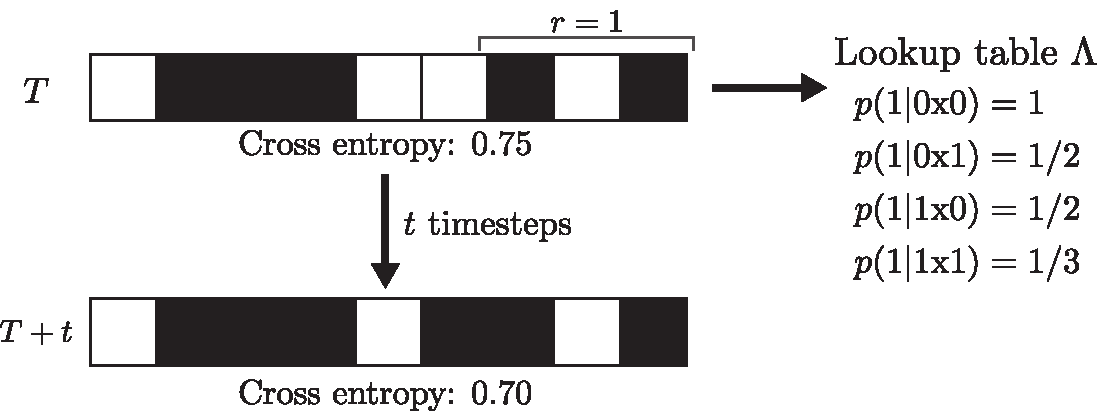
\includegraphics[width=.7\linewidth]{figures/schema-count}
  \caption{Count-based predictor method for a radius $r=1$. A
    frequency lookup table is computed from the global state at time $T$ by
    considering all neighborhoods with radius $r=1$ (3 consecutive cells
    but ignoring the middle cell). Cross-entropy with the automaton at time $T$
    quantifies the overall complexity. This can be compared to the cross-entropy
    at time $T + t$ for the amount of overlap.}
  \label{fig:schema-count}
\end{figure}

We apply this metric to all 256 ECA, with a window radius of size 3 (the 6
closest neighbors are used for prediction), and the same settings as for
Figure~\ref{subfig:comp_scores}. Cross-entropy loss of the lookup table gives
the results of Figure~\ref{subfig:cross_ent_one}. Colors are the same as in
Figure \ref{subfig:comp_scores} for comparison purposes.

\begin{figure}[htbp]
  \centering
  \subfloat[Count-based predictor]{
    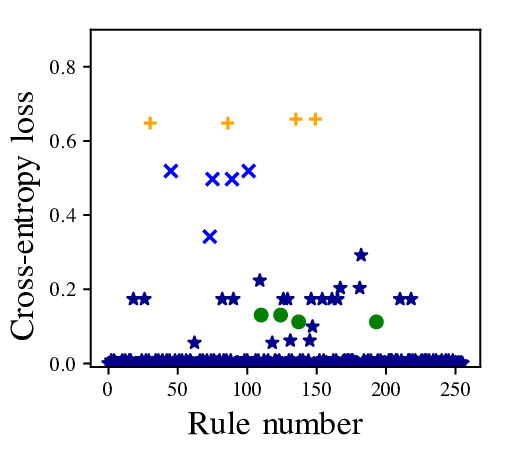
\includegraphics[width=.405\linewidth]{figures/count}
      \label{subfig:cross_ent_one}
  }\hfil
  \subfloat[Neural network-based predictor]{
    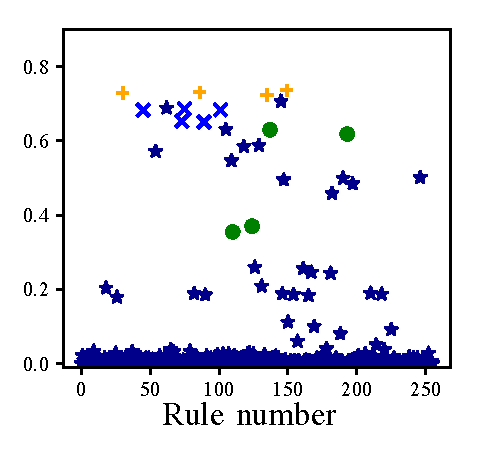
\includegraphics[width=.38\linewidth]{figures/nn}
      \label{subfig:nn_ent_one}
  }
  \caption{Average cross entropy loss for the two predictor-based methods on all
    256 ECA. Rules are separated in several clusters. The
    count-based predictor (left plot) and neural network-based predictor (right
    plot) were applied with a neighborhood radius $r=1$ and $3$.}
\end{figure}

We note the similarity between this plot and the one from Figure
\ref{subfig:comp_scores}, with a roughly equivalent resulting classification of
ECA rules, with the exception of rules with low score. Rules that produce highly
disordered patterns are on top of the plot whereas the very simply behaving
rules are at the bottom. This indicates coherence between the two metrics.

\subsection{Neural network based predictor}

\begin{figure}[htbp]
  \centering
  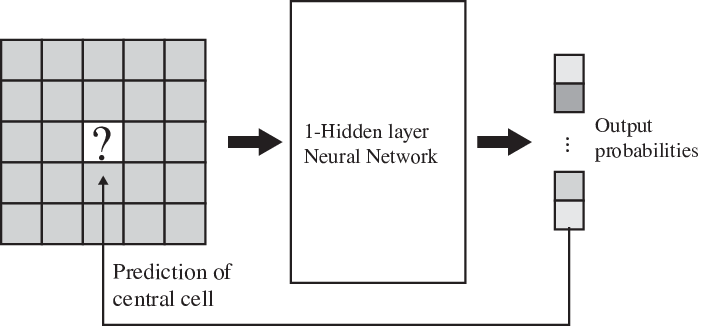
\includegraphics[width=.7\linewidth]{figures/nn_archi}
  \caption{Neural network architecture for predicting a central cell given its
    neighbors. Output probabilities are defined for all possible states of the
    central cell.}
  \label{fig:nn_archi}
\end{figure}

The frequency based predictor described above still has limitations:
\begin{itemize}
\item It doesn't take into account any redundancy in the input which may lead to
  suboptimal predictions (in a CA, very similar positions might have similar
  center cell state distribution, e.g. a glider in Game of Life should be
  recognized by the model no matter the rest of the neighborhood).
\item For the same reasons, when considering large window sizes, the number of
  possible neighborhood configuration gets much larger than the number of
  observed ones, leading to an input sparsity problem.
\end{itemize}
More sophisticated models can cope with above limitations by dealing with high
dimensional inputs without sparsity problems, and taking into account redundancy
of inputs and potential interactions between states for prediction.

We measure the cross-entropy loss of this simple model on the training set after
a standard learning procedure which is the same for all rules. The procedure is
applied to a one hidden layer neural network with a fixed hidden layer size. We
use a ReLU non-linearity for the hidden layer and a softmax to obtain the output
probabilities.

For $n$ possible states ${s_1, ..., s_n}$, a cell in state $s_k$ is represented
as a vector of 0s of size $n$ with a 1 in position $k$. The input to the network
is the concatenation of these cell vectors for all cells in the neighborhood.
The output of the network is a vector of size $n$ with the output probability
for each state.

Gradient updates are computed during training to minimize the cross-entropy loss
between outputs and target examples. For a timestep $T$, we use the training
procedure in order to minimize with respect to $\theta$ the following quantity,
\begin{align}
  L_\theta^{(T)} = - \frac{1}{N}\sum_{i=1}^N \sum_{k=1}^n
  \mathds{1}_{\{ s_k \}}\left(c_i^{(T)}\right)
  \log\left[f_\theta\left(n_{r,i}^{(T)}\right)_{s_k}\right]
  \label{eq:loss_network}
\end{align}
where the neural network depending on parameter $\theta$ is denoted $f_\theta$,
and $n_{r,i}^{(T)}$, the neighborhood of cell $i$ with radius $r$ at time $T$ is
defined in the same way as in eq.~\eqref{eq:loss_count}. Loss is computed with
respect to the testing set at time $T + \tau$ by computing the same quantity at
this subsequent timestep.

The training procedure is selected to achieve reasonable convergence of the loss
for the tested examples. It must be well defined and stay the same to allow for
comparison of the results across several rules. Score at timestep $T$ for a
delay $\tau$ is computed with the following formula
\begin{align}
  \textstyle \mu_\tau = \dfrac{L^{(T)}}{L^{(T + \tau)}}
  \label{eq:main_metric}
\end{align}
where $L^{(T + \tau)}$ is the log probability of the automaton state at timestep
$T + \tau$ (defined in eq.~\eqref{eq:loss_network}) according to a model with
parameters learned during training at timestep $T$ and $L^{(T)}$ is the same as
in eq.~\eqref{eq:loss_network}. The value $\mu_\tau$ will be lower for easily
``learnable'' global states that do not translate well in future steps --- they
create more complexity or disorder --- thereby discarding slowly growing very
disordered structures. Higher values of $\mu_\tau$ correspond to automata that
have a disordered global state at time $T$ that can be transposed to future
timesteps relatively well. Those rules will tend to have interesting spatial
properties --- not trivially simple but not completely disordered because the
model transposes well --- as well as a large amount of overlap between a given
step and the future ones, indicating persistence of the spatial properties from
one state to another. We also selected the metric among other quantities
computed from $L^{(T)}$ and $L^{(T+\tau)}$ because it yielded the best score on
our experimental datasets.

\section{Experiments}\label{sec:experiments}

We carried out several experiments on a dataset of 500 randomly generated 3
states ($n=3$) rules with radius $r=1$. Those rules were manually annotated for
interestingness, defined as the presence of visually detectable non trivial
structures. The dataset contains 46 rules labeled as interesting and 454
uninteresting rules. Ranking those rules with the metrics introduced above
allows to study the influence of parameters and the adequacy between
interestingness as we understand it and what the metric measures.

The task of finding interesting rules can either be framed as a classification
problem or a ranking problem with respect to the score we compute on the
dataset. The performance of our metric can be measured with usual evaluation
metrics used on these problems, and notably the average precision (AP) of the
resulting classifier.

Average precision scores for the neural network and count-based methods for time
windows of 5, 50 and 300 timesteps are given in Table~\ref{experiments_table}.
Scores were computed on automata of size $256\times 256$ cells, ran for 1000
timesteps ($T + \tau = 1000$). Scores were computed for radii ranging from 1
cell (8 nearest neighbors) to 5 cells (120 neighbors), with a one layer neural
network containing 10 hidden units trained for 30 epochs with batches
of 8 examples. Best AP for each time window is shown in bold.
Results for the frequency lookup table predictor are only shown for $r=1, 2$
because of sparsity issues with the lookup table from $r=2$ and above making it
unpractical to use the table --- $3^{24}$ possible entries for the lookup table
with $r=2$ against only $256^2$ observed states.

\begin{table}[t!]
  \renewcommand{\arraystretch}{1}
  \caption{Experimental results - AP scores}
  \label{experiments_table}
  \centering
  \begin{tabular}{c|c|c|c|c|c}
    \toprule
    \bfseries Neural network& $r=1$ &  2  & 3  & 4 & 5\\
    \midrule
    5 steps & 0.387 & 0.448 & \bfseries 0.541 & 0.525 & 0.534\\
    50 steps & 0.377 & 0.433 & 0.517 & 0.491 & \bfseries 0.542\\
    300 steps &0.358 & 0.454 & 0.488 & \bfseries 0.527 & 0.525\\
    \midrule
    \bfseries Lookup table& $r=1$ &  2  & & &\\
    \midrule
    5 steps & 0.092 & 0.070&&&\\
    50 steps & 0.102 & 0.070&&&\\
    300 steps & 0.093 & 0.069&&&\\
    \bottomrule
  \end{tabular}

  \begin{flushleft}{This table shows the average precision (AP)
      scores obtained on the dataset of section \ref{sec:experiments} with the
      neural network-based and lookup table-based methods. Results are show for
      delays $\tau = 5, 50, 300$ and several radii values $r$.}\end{flushleft}
\end{table}

From these experiments, bigger radii appear to perform slightly better, although
not in a radical way. Since the number of neighbors scales with the square of
the radius, reasonably small radii might be a good trade-off between performance
and computational cost of the metric.

We also study the performance of our metrics --- lookup table and neural
network-based --- as inputs of a binary classifier against two simple baselines
on a random 70/30 split of our dataset. The first baseline classifies all
example as negative. The second baseline is based on compressed length as
defined in \cite{zenil_compression-based_2010} and computed by choosing a pair
of thresholds that minimize mean square error when classifying examples in
between as positive --- this is based on the observation made in
Section~\ref{sec:compr-based-metr} that interesting rules have intermediate
compressed lengths. Results are in Table~\ref{experiments_table2} where only the
best radius is shown. The lookup table performs better than the baselines but
the neural network gives the best score.

\begin{table}[t!]
  \renewcommand{\arraystretch}{1.2}
  \caption{Experimental results - Accuracy}
  \label{experiments_table2}
  \centering
  \begin{tabular}{lm{.1\linewidth}m{.16\linewidth}m{.1\linewidth}m{.11\linewidth}}
    \toprule
    \bfseries  Metric & Baseline & Compressed length
    \cite{zenil_compression-based_2010} &
    Lookup Table & Neural network \\ \midrule
    \bfseries Accuracy & 0.90 & 0.913 & 0.926 & \bfseries 0.953 \\ \bottomrule
  \end{tabular}
  \\[+8pt]
  \begin{flushleft}{\footnotesize Accuracy of each metric of complexity when
      used to classify which automatons do evolve interestingly, compared
      against the trivial all-negative baseline and the compressed length
      metric~\cite{zenil_compression-based_2010}.}\end{flushleft}
\end{table}

Above experiments demonstrate the capability of our proposed metric to match a
subjective notion of interestingness of our labeling. For instance, the top 5
and top 10 scoring rules of the best performing configuration ($r=3$, $\tau =
5$) are all labeled as interesting, and top 100 scores contain 41 of the 46
rules labeled as interesting.

\section{Discussion}

In this section, we discuss the results obtained by using the metric of equation
\eqref{eq:main_metric} and the way they can be interpreted.

\paragraph{One dimensional cellular automata}
By applying the metric on the same example as before, we again obtain a
plot with a rule classification that matches a visual appreciation of
complexity of 1D CA. Results are shown on Figure~\ref{subfig:nn_ent_one}.
Similarly to the previous cases, rules we might label as interesting are
unlikely to be either at the top or bottom of the plot.

\paragraph{Two dimensional cellular automata}

Simulations conducted with 2D CA used grids of size 256$\times$256. Automata
were ran for 1000 steps (the metric is measured with respect to the reference
time $T = 1000$). Rules are defined with a table of transitions from all
possible neighborhood configurations with radius $r=1$ (3$\times$3 squares) to a
new state for the central cell. Unbiased sampling of rules, obtained by
uniformly sampling the resulting state for each transition independently,
overwhelmingly produces rules with a similar amount of transitions towards each
state and fails to produce rules without completely disordered behavior more
than 99\% of the time.

Therefore, we adopt a biased sampling strategy of the rules, selecting the
proportion of transitions towards each state uniformly on the simplex --- e.g
for 3 states we might get the triple $(0.1, 0.5, 0.4)$ and sample transitions
according to these proportions. This parametrization can be related to Langton's
lambda parameter \cite{langton_computation_1990} that takes into account the
proportion of transitions towards a transient (inactive) state and all the other
states. We obtain approximately 10\% interesting rules with this sampling as the
proportions of our experimental dataset show.

\begin{figure}[t]
  \centering
  \subfloat{
    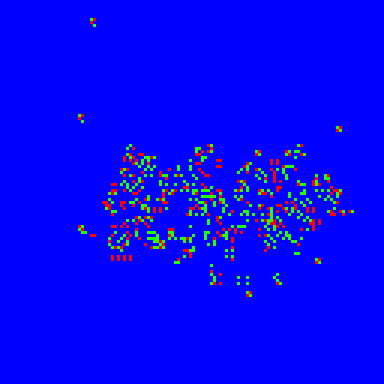
\includegraphics[width=.38\linewidth]{figures/glid1}
  }\hfil
  \subfloat{
    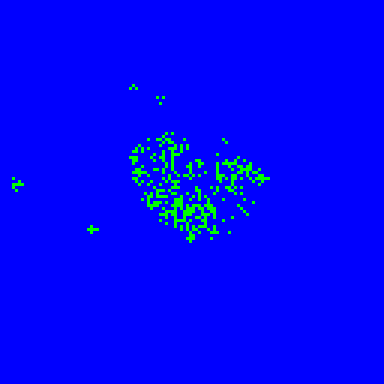
\includegraphics[width=.38\linewidth]{figures/glid2}
  }
  \caption{Rules with 3 states that have spontaneously occurring glider
    structures. The gliders are the small structures that are outside of the
    center disordered zone. Some of them move along the diagonals while some
    others follow horizontal or vertical paths. Note that some repeating
    patterns occur also in the more disordered center zone.}
  \label{fig:gliders}
\end{figure}

\begin{figure}[t]
  \centering
  \subfloat{
    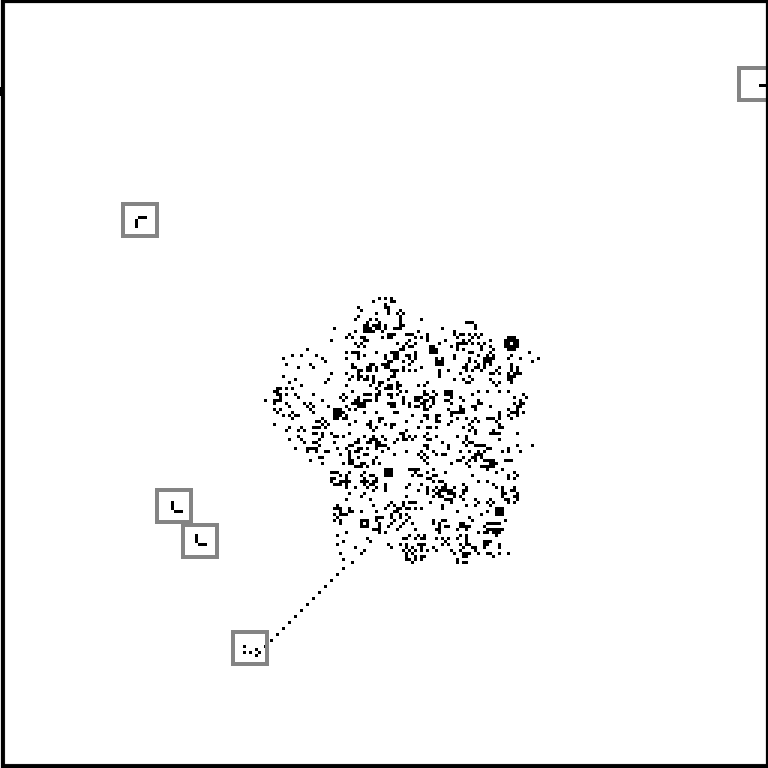
\includegraphics[width=.38\linewidth]{figures/2d_b_1}
  }\hfil
  \subfloat{
    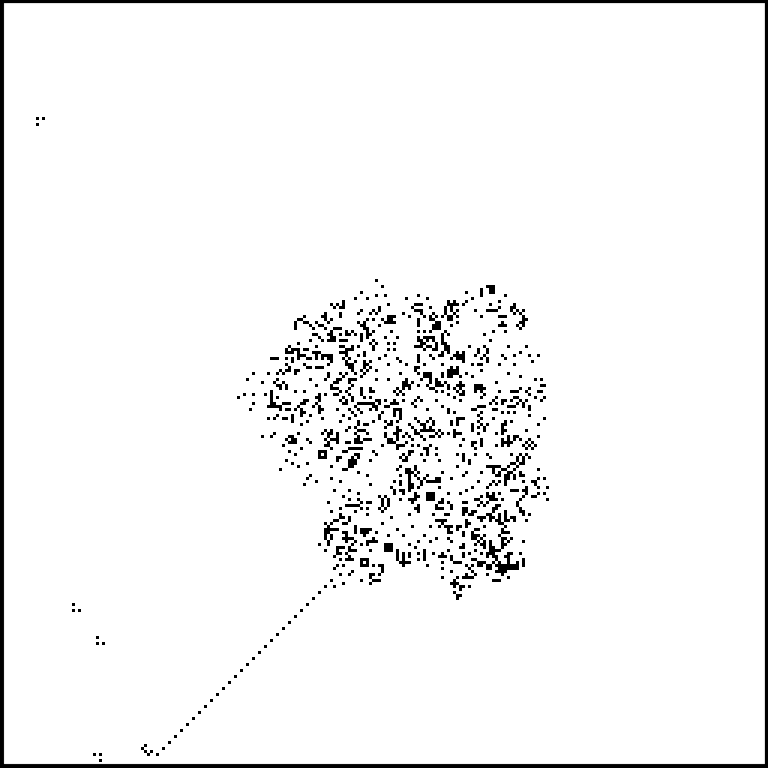
\includegraphics[width=.38\linewidth]{figures/2d_b_2}
  }\hfil\setcounter{subfigure}{0} % Get the numbers right
  \subfloat[Timestep $T$]{
    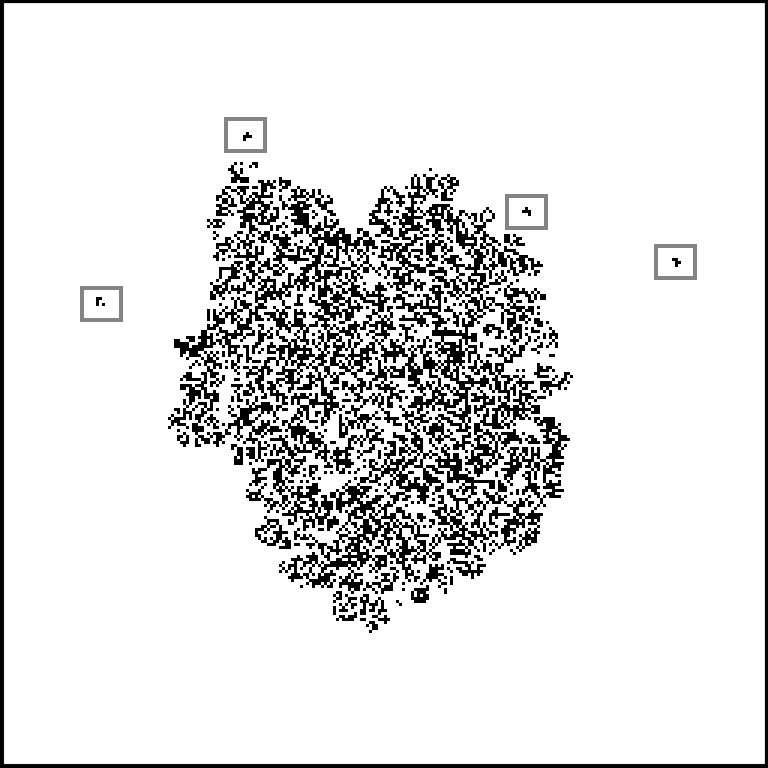
\includegraphics[width=.38\linewidth]{figures/2d_c_1}
  }\hfil
  \subfloat[Timestep $T + 50$]{
    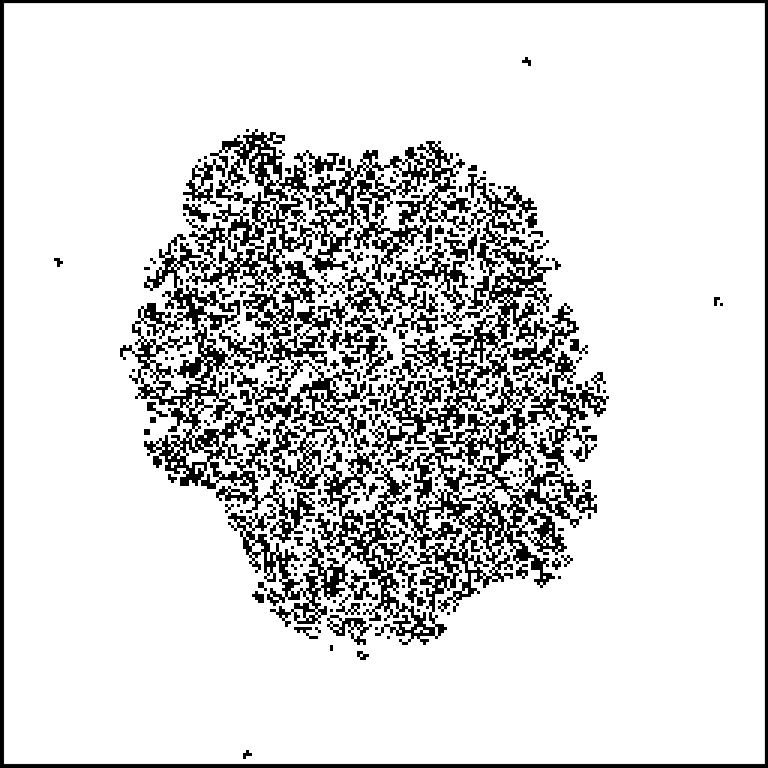
\includegraphics[width=.38\linewidth]{figures/2d_c_2}
  }
  \caption{Spontaneous glider formation and evolution is observed for some high
    scoring 2 states rules. Each row corresponds to a rule, with a 50 timesteps
    difference between the two columns. Gliders are marked with a gray square.
    Runs were initialized with a small 20 by 20 disordered square (uniformly
    sampled among possible configuration) in the center simulated for up to 400
    steps.}
  \label{fig:automat_glider}
\end{figure}

Using the neural network-based complexity metric, we were able to find rules
with interesting behavior among a very large set through random sampling. Some
of these rules are shown in the paper. Figure~\ref{fig:automat_glider} displays
three 2D rules that were selected manually upon visual inspection among the 20
highest scoring for metric $\mu_{50}$ (defined in eq.~\eqref{eq:main_metric}) of
a sample of 1700 randomly generated 2-states 3 by 3 neighborhood rules. For
comparison, Conway's Game of Life rule (GoL) ranks in the top 1\% of the 2500
rules mentioned above for runs that don't end in a static global state. We
observe that spontaneous glider formation events appear to be captured by our
metric. Although gliders in cellular automata are a simple process that can
manually be created, detection of their spontaneous emergence within a random
search setting is a first step towards finding more complex macro structures
that can emerge out of simple components. Rules with low scores are
overwhelmingly of the disordered kind.

Figures~\ref{fig:gliders}, \ref{fig:micro} and \ref{fig:odd} show some three
states rules that were selected through random sampling on the simplex with the
neural-network based metric. They were selected among the 30 highest scoring
rules out of 2500 randomly selected 3 states rules. Their behaviors all involve
the growth and interaction of some small structures made of elementary cells.

All automata were initialized with a random disordered square of 20 by 20 cells
in the center. In the Figures mentioned above, colors were normalized with the
most common state set to blue. Figure~\ref{fig:gliders} shows rules that
spontaneously emit gliders that go through space in a direction until they
interact with some other active part of the automaton. Figure~\ref{fig:micro}
shows rules that generate small structures of between four and thirty cells that
are relatively stable and interact with each other. These elementary components
could be a basis for the spontaneous construction of more complex and bigger
components. Figure~\ref{fig:odd} shows some other rules from this set of high
ranking automata. They highlight the wide range of behaviors that can be
obtained with these systems. Interesting rules from this paper can be found,
along with other examples, in the form of animated
GIFs\footnote{\url{https://bit.ly/interesting_automata}}.

\begin{figure}[t]
  \centering
  \subfloat{
    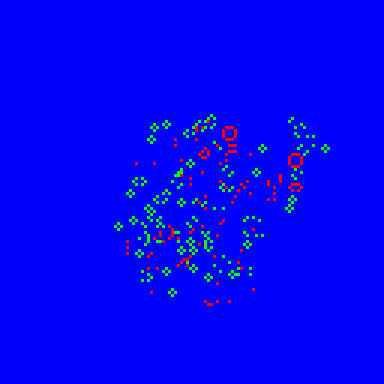
\includegraphics[width=.38\linewidth]{figures/micro3}
  }
  \hfil
  \subfloat{
    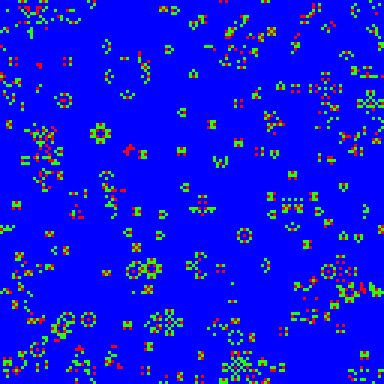
\includegraphics[width=.38\linewidth]{figures/micro4}
  }
  \caption{Rules with 3 states that generate cell-like interacting structures.
    These patterns are either static or moving and can interact with one another
    to generate copies of themselves and other patterns. Note the very similar
    micro-structures that are repeated at several places in the space.}
  \label{fig:micro}
\end{figure}


\begin{figure}
  \centering
  \subfloat{
    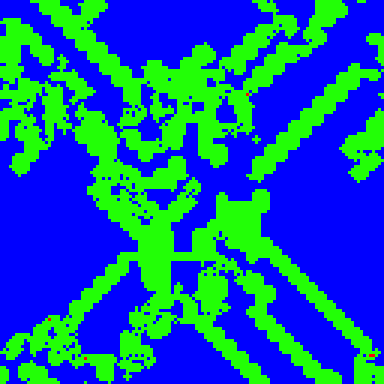
\includegraphics[width=.38\linewidth]{figures/odd1}
  }
  \hfil
  \subfloat{
    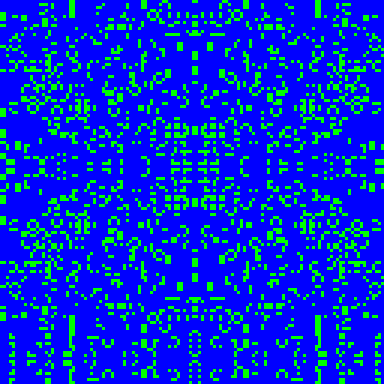
\includegraphics[width=.38\linewidth]{figures/odd2}
  }
  \caption{Rules with surprising behaviors that are highly structured but
    complex. Those rules were selected among high-ranking rules for the
    neural-network based complexity metric. They all exhibit structurally non
    trivial behavior.}
  \label{fig:odd}
\end{figure}

For some of these rules interesting patterns appear less frequently in smaller
grids, indicating that the size of the space might impact the ability to
generate complex macro-structures. Increasing the size of the state space to
very large grids might therefore make it easier generating very complex patterns.

\section{Conclusion}\label{sec:conclusion}

In this paper, we have proposed compression-inspired metrics for measuring a
form of complexity occurring in complex systems. We demonstrated its usefulness
for selecting CA rules that generate interesting emergent structures from very
large sets of possible rules. In higher dimensions where linear compression ---
as in gzip --- is not sufficient to find complex patterns, our metric is also
useful.

We study 2 and 3 states automata in the paper and we plan to investigate the
effects of additional states or larger neighborhoods on the ability to evolve
more structures and obtain more interesting behaviors.

In the future, we will publish the dataset and code to enable reproducibility
and improvement on the results reported
here\footnote{\url{https://github.com/hugcis/evolving-structures-in-complex-systems}}.
The metrics we introduce in this paper could be used to design organized systems
of artificial developing organisms that grow in complexity through an
evolutionary mechanism. A possible path toward such systems could start by
creating an environment where computational resource allocation favors the
fraction of subsystems that perform the best according to our measure of
complexity.

The proposed metric is theoretically applicable to any complex system where a
notion of state of an elementary component and locality can be defined. With
these requirements fulfilled, we can build a similar prediction model that uses
information about local neighbors to predict the state of a component and
thereby assess the structural complexity of an input.

We believe that the capability of creating evolving systems out of such
elementary components and with few assumptions could be a step towards AGI. By
devising ways to guide this evolution in a direction we find useful, we would be
able to find efficient solution to hard problems while retaining adaptability of
the system. It might be suitable to avoid over-specialization that can happen in
systems designed to solve a particular task --- e.g. reinforcement learning
algorithms that can play games, and supervised learning --- by staying away from
any sort of objective function to optimize and by leaving room for open-ended
evolution.

\chapter{Visualization of computation in large-scale complex systems}
\label{cha:visu-comp-large}

  Emergent processes in complex systems such as cellular automata can perform
  computations of increasing complexity, and could possibly lead to artificial
  evolution. Such a feat would require scaling up current simulation sizes to
  allow for enough computational capacity. Understanding complex computations
  happening in cellular automata and other systems capable of emergence poses
  many challenges, especially in large-scale systems. We propose methods for
  coarse-graining cellular automata based on frequency analysis of cell states,
  clustering and autoencoders. These innovative techniques facilitate the
  discovery of large-scale structure formation and complexity analysis in those
  systems. They emphasize interesting behaviors in elementary cellular automata
  while filtering out background patterns. Moreover, our methods reduce large 2D
  automata to smaller sizes and enable identifying systems that behave
  interestingly at multiple scales.

\section{Introduction}
Cellular automata (CA) have been extensively studied since the 1960s. Originally
designed and studied to create artificial evolution from self-replication
\parencite{vonneumannTheorySelfreproducingAutomata1966,
  langtonSelfreproductionCellularAutomata1984}, previously studied cellular
automata simulations were often of relatively modest sizes. Only specific rules
with repetitive or predictable dynamics such as John Conway's Game of Life
\parencite{gardnerMathematicalGames1970} have been scaled up to larger grid sizes
($10^4 \times 10^4$ or more cells).

For complex phenomena such as artificial evolution to exist and be open-ended
within those simulated worlds, there needs to be sufficient ``capacity'' --- a
large enough state-space. In nature, complex and significantly different
dynamics often arise from uniform laws at a smaller
scale~\parencite{andersonMoreDifferent1972}. It seems unlikely that such complex
processes, like artificial evolution, could happen in too small CAs because
higher order dynamics do not have enough capacity to emerge. However, several
issues arise when scaling CAs to large sizes:

\begin{itemize}
\item Time complexity rapidly becomes a bottleneck. Updating a large number of
  cells is costly. Tricks such as caching of some of the computations can help,
  but do not always improve performance
  significantly~\parencite{gosperExploitingRegularitiesLarge1984}.

\item Memory complexity can also become an issue when dealing with numerous
  states, and especially grids in 3 dimensions and more. In that case, even the
  underlying rule of the system cannot be stored within reasonable memory
  capacity.

\item Visual inspection of these large grids is infeasible. Studying CA
  complexity is rendered difficult by the highly variable nature of emergent
  processes. It is especially the case for large-scale systems.

\end{itemize}
When working with such large systems, it is less relevant to focus on the local
behaviors at the single cell level. This is similar to other complex systems
like the weather, in which behaviors of individual atoms in a cloud are
irrelevant to large-scale air mass movements. Much richer behaviors can be
observed from studying large patterns' formation and their evolution. This
should also hold true for CAs; we further discuss this question in
\nameref{sec:conclusion-vc}.

\begin{figure}[th]
  \centering
  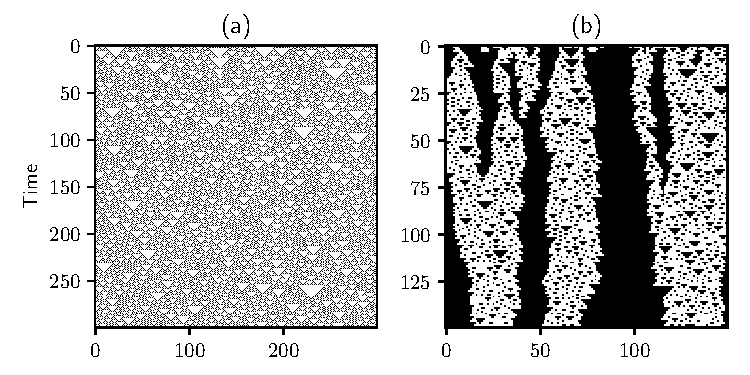
\includegraphics[width=.93\linewidth]{figures/rule18_small.pdf}
  \caption{\label{fig:rule18_small} \textbf{Hidden structures in rule 18 are
      uncovered by filtering the space-time diagram with our frequency
      histogram-based method}. \textbf{(a)} shows 300 timesteps of a randomly
    initialized rule 18 simulation. Notice the complex structures made visible
    in \textbf{(b)} with our method.}
\end{figure}

In this paper, we investigate techniques which can help us visualize large
space-time diagrams of CAs. We demonstrate that simple clustering and
coarse-graining techniques can be used in order to perceive structures which
cannot emerge on smaller grids. This is also useful for disordered cellular
automata with hidden structures as it is the case for the elementary cellular
automaton rule 18, illustrated in Figure~\ref{fig:rule18_small} --- more details
in~\nameref{sec:results}.

Reducing large grids to smaller sizes while preserving interesting behaviors
such as pattern formation is essential to apply to these CAs complexity metrics
designed to work on modestly sized
grids~\parencite{grassbergerQuantitativeTheorySelfgenerated1986,
  zenilCompressionBasedInvestigationDynamical2010,
  soler-toscanoCalculatingKolmogorovComplexity2014,
  zenilTwodimensionalKolmogorovComplexity2015}. Common metrics of complexity are
often limited by the number of components in the systems (number of cells in a
CA grid, timesteps, etc.) or may not be effective when small scale patterns are
less relevant than large-scale ones.

\section{Related work}

Previous work on coarse-graining cellular automata focused either on conserving
the main computational properties of CA rules through exact coarse-graining or
on filtering interesting behaviors without reducing the amount of computations.
Our work both highlights interesting behaviors and compresses the
representation, which we argue are necessary to study complexity in large
cellular automata.

\subsection{Coarse-graining in cellular automata}
Coarse-graining is an approximation procedure used to speed up computations in
systems made of many components. It originated
in~\parencite{levittComputerSimulationProtein1975} and is now widely used in physics
to model complex systems at various granularity levels, and is successful at
modeling bio-molecules \parencite{potoyanRecentSuccessesCoarsegrained2013,
  ingolfssonPowerCoarseGraining2014, kmiecikCoarseGrainedProteinModels2016}.

Exact coarse-graining of elementary cellular automata (ECA) has been
investigated extensively
in~\parencite{israeliComputationalIrreducibilityPredictability2004,
  israeliCoarsegrainingCellularAutomata2006}. Authors found ways of rewriting
one-dimensional CA rules into each other through coarse-graining of the
transition rule. They built a graph of equivalence of all 256 ECA and identified
some rules that do not admit any computational reduction. This indicates that
some cellular automata are accomplishing fundamentally more computations than
others.

\subsection{Filtering}

Filtering cellular automata (CA) was introduced to reduce a CA's behavior to its
most relevant parts. The goal is to extract relevant irregularities from a CA's
space-time diagram. Seminal work
by~\parencite{hansonAttractorbasinPortraitCellular1992,
  hansonComputationalMechanicsCellular1997} formalized the notion of domains and
coherent structures in cellular automata. They used a set of regular languages to
represent cellular automata dynamics and extract relevant behaviors such as
discontinuities between regular domains or ``particles''.
Figure~\ref{fig:rule110} shows a filtering example for cellular automaton rule
110 --- in Wolfram's numbering.

A filtering method similar to our proposed frequency-based coarse-graining ---
originally presented as a complexity metric for cellular automata --- is
introduced in~\parencite{wuenscheClassifyingCellularAutomata1999}. The author
proposes to progressively filter out cells in cellular automata's space-time
diagrams according to read frequency of the rule table. Cells that originated
from frequent rule table lookups are set to a quiescent or null state. The
choice of threshold has to be decided by a user for each rule. Another notable
difference is the method aims at making visualization of gliders easier without
reducing the size of the grid or making more compact representations.

More recent work by~\parencite{shaliziAutomaticFiltersDetection2006} uses the
combination of a modified Lyapunov exponent approach with \emph{statistical
  complexity} \parencite{shaliziQuantifyingSelfOrganizationOptimal2004} to underline
complex behaviors. However, the first method requires repeated perturbations and
simulations of the system to study its sensitivity.

\subsection{Scaling-up cellular automata}
Hashlife \parencite{gosperExploitingRegularitiesLarge1984} and other Game of
Life-specific optimizations enable simulating a large number of cells for
numerous timesteps. Nonetheless, these algorithms essentially exploit input
redundancy. The regularity in patterns allowing such optimizations might
indicate a lack of novel patterns being generated by the system.

This also means that Game of Life-based simulations are computationally
reducible to a much simpler system, indicating that its computations are
inefficient~\parencite{wolframNewKindScience2002}. An optimally complex-behaving
computational model should be impossible to predict except when computing its
actual evolution step by step.

In the following, we used coarse-graining as a method for scaling down CAs in
both time and space in order to make visualization of larger patterns and
complex behaviors easier. The underlying fine-scale computations may be
essential for these larger patterns to appear, hence the necessity to keep them.
However, analogous to many natural processes (swarms, chemistry, cells in an
organism, DNA), interesting behaviors might not be observable at the level of
individual components --- or small groups of components (individuals, single
cells or molecules in the examples above). We view coarse-graining as a way to
reduce a cellular automaton's space-time diagram to its most relevant parts
while keeping primary dynamics in the background. The resulting diagram would
ideally be an irreducible system.

\section{Proposed coarse-graining of cellular automata}
For reasons stated above, we introduce coarse-graining methods for cellular
automata that are not reversible --- information is discarded in the process.
This process does not attempt to find shortcuts for the computations of a
cellular automaton, but rather to selects relevant parts of the space-time
diagram and discards information irrelevant to the core behavior. For example, a
standard glider in Game of Life spanning $3\times 3$ cells could be replaced
with a single cell moving diagonally when coarse-graining by a factor 3. This is
because the actual oscillator's dynamics might not be relevant at this coarser
scale.

Coarse-graining is akin to constructing \emph{supercells} from blocks of individual
cells. These supercells are assigned a new state and form a coarser partitioning
of the initial grid which can be studied as its own system. In particular,
complexity metrics or further coarse-graining can be applied to this new grid.

\subsection{Frequency histogram coarse-graining}\label{sec:simple-hier-coarse}

A simple coarse-graining is achieved by mapping blocks to a single
\emph{supercell} state according to the probability of this configuration
appearing, given a previously constructed model. The easiest way to think of it
is with a simple frequency counting model of the distribution of $2\times 2$
blocks in a 2D CA\@. For a 2-state automaton, there are 16 possible supercell
configurations. The simplest model for the occurrence of these blocks is their
empirical frequency. Let us consider a CA with $N$ blocks of $2\times 2$ cells,
let $S^{(in)} = \{\mathtt{0000}, \mathtt{0001}, \mathtt{0010}, \ldots,
\mathtt{1111}\}$ be the set of $2\times 2$ blocks and $s_i \in S^{(in)}$ be a
given supercell. The probability $p_i$ of observing supercell $i$ on a grid $G$
is estimated with
\begin{equation}
  p_i = \dfrac{\text{count}_G(s_i)}{\sum_{j\in S^{(in)}}\text{count}_G(s_j)}
  \label{eq:stat_est}
\end{equation}
where $\text{count}_G(s_i)$ is the number of blocks matching $(s_i)$ in $G$.

Supercells can then be assigned a particular state. We call the corresponding
mapping $f: S^{(in)} \mapsto S^{(out)}$. $S^{(out)}$ can be chosen depending on
the desired output or use. For instance, with $S^{(out)} = \{0, 1\}$ we can
define $f$ to map each supercell $s_i$ as follows:
\begin{align}
  f(i) = \begin{cases}
    \mathtt{0} &\quad\text{if }\ p_i\geq \alpha\\
    \mathtt{1} &\quad\text{if }\ p_i< \alpha
  \end{cases}
        \label{eq:alpha}
\end{align}
where $\alpha$ is a chosen threshold.

\subsubsection{Partitioning the histogram.}
This method can be understood as partitioning the histogram of supercell
frequency. In equation~\eqref{eq:alpha}, supercells with low probability
--- with higher self-information --- are mapped to state \texttt{1} whereas
commonly occurring states are mapped to \texttt{0}.

Choosing a partition of the histogram is equivalent to selecting a suitable
$\alpha$ --- scalar for two output states, or vector $\mathbf{\alpha} =
(\alpha_1, \ldots, \alpha_n)$ for $n$ output states. Therefore, one can map
supercells to any number of target states (three or more) by partitioning the
frequency histogram into any number of bins. Supercell distribution can be
anything between uniform and very unbalanced, with a few supercells being
overwhelmingly represented (background) and only a few occurrences of other
configurations. The chosen partitioning has to deal with both situations equally
well. In the following, we use a uniform partitioning of the area under the
negative log-histogram for elementary cellular automata --- supercells are
divided into two bins of equal summed negative logarithmic probability. For 2D
CAs, we use the same method but with quadratic partition of the histogram
($1/k^2$ instead of $1/k$, with $k$ the number of output states, chosen because
of better visual results).

\subsubsection{Dithering.}\label{sec:dithering}
Histogram partitioning introduces another set of parameters to be manually
tuned, adding complexity to the procedure. An alternative way to produce an
output image from the histogram is to use dithering. Dithering is an image
processing technique commonly used to reduce large visual artifacts induced by
quantization errors. Noise is added to the image during the quantization process
to make the average local value of a set of pixels as close to their target
continuous value as possible. The resulting image is created so as to match
target continuous values with discrete values only --- cell states in the grid.
It can be seen as another way of partitioning the histogram with variable
thresholds that depend on a running quantization error.
Figure~\ref{fig:close-up} shows a comparison of dithering and regular histogram
partitioning (Floyd–Steinberg's algorithm was used
\parencite{floydAdaptiveAlgorithmSpatial1976}).

\setlength{\fboxsep}{0pt}
\begin{figure}[th]
  \centering
  \begin{subfigure}{.32\linewidth}
    \fbox{\centering
    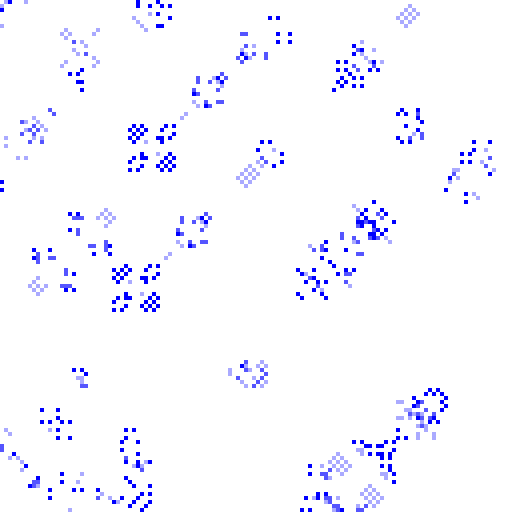
\includegraphics[width=\linewidth]{figures/step_large.png}}
    \caption{\label{subfig:normal}Original CA}
  \end{subfigure}
  \hfill
  \begin{subfigure}{.32\linewidth}
    \fbox{\centering
    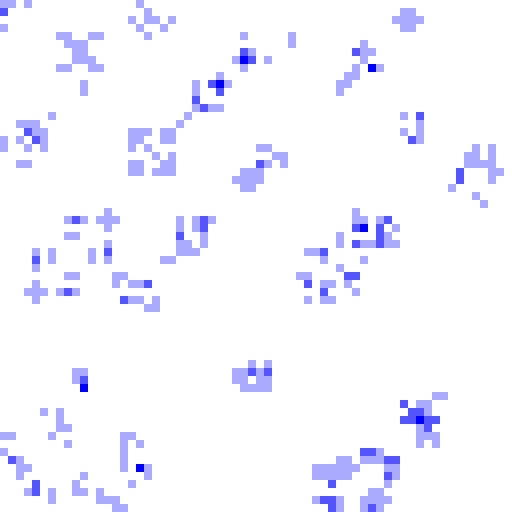
\includegraphics[width=\linewidth]{figures/freq_cg_large.png}}
    \caption{\label{subfig:no-dithering}w/out dithering}
  \end{subfigure}
  \hfill
  \begin{subfigure}{.32\linewidth}
    \fbox{\centering
    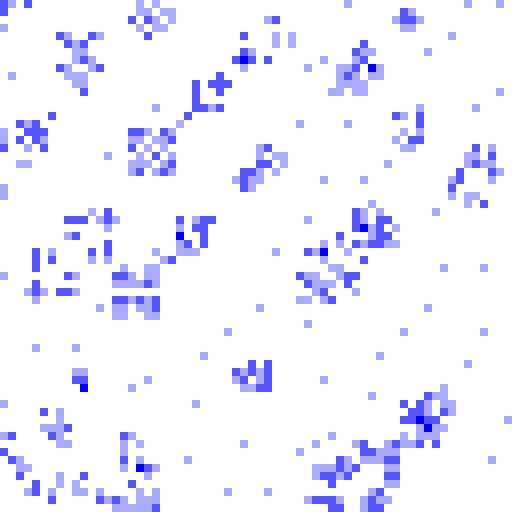
\includegraphics[width=\linewidth]{figures/dither_cg_large.png}}
    \caption{\label{subfig:dithering}with dithering}
  \end{subfigure}

  \caption{\label{fig:close-up}\textbf{Close-up view of coarse-graining effects
      on a 4-states CA rule} (1 shade of blue per state). Both coarse-graining
    methods conserve many of the interesting structures. Dithering introduces
    additional artifacts on regular backgrounds. Fig.~\ref{subfig:normal} shows
    actual states in the CA simulation on a $128 \times 128$ grid.
    Fig.~\ref{subfig:no-dithering} is a coarse-grained version
    of~\ref{subfig:normal} with histogram coarse-graining, the grid is $64
    \times 64$ cells.\ref{subfig:dithering} is obtained with histogram
    coarse-graining and dithering (see \nameref{sec:dithering}).}
\end{figure}


\subsubsection{Visualization.}
One advantage of this frequency histogram-based method is that it naturally
highlights rarer events in the simulation grid, creating a ``heatmap'' of the
simulation's activity. Since we sort supercells according to their observed
frequency, the right choice of colors --- e.g.\ progressively darker gradient
--- can lead to automatic highlighting of active regions of a cellular
automaton. Figure~\ref{fig:gol_comparison} shows the same simulation both
unprocessed and downscaled by a factor of 4 with coarse-graining. Although much
coarser, Figure~\ref{subfig:gol_cg} is more readable than the base version,
which is helpful when dealing with large grids\footnote{Several figures in this
  paper have animated versions, accessible at the paper's project page
  \projecturl}.

\begin{figure}[th]
  \centering
  \begin{subfigure}{.48\linewidth}
    \fbox{
    \centering
    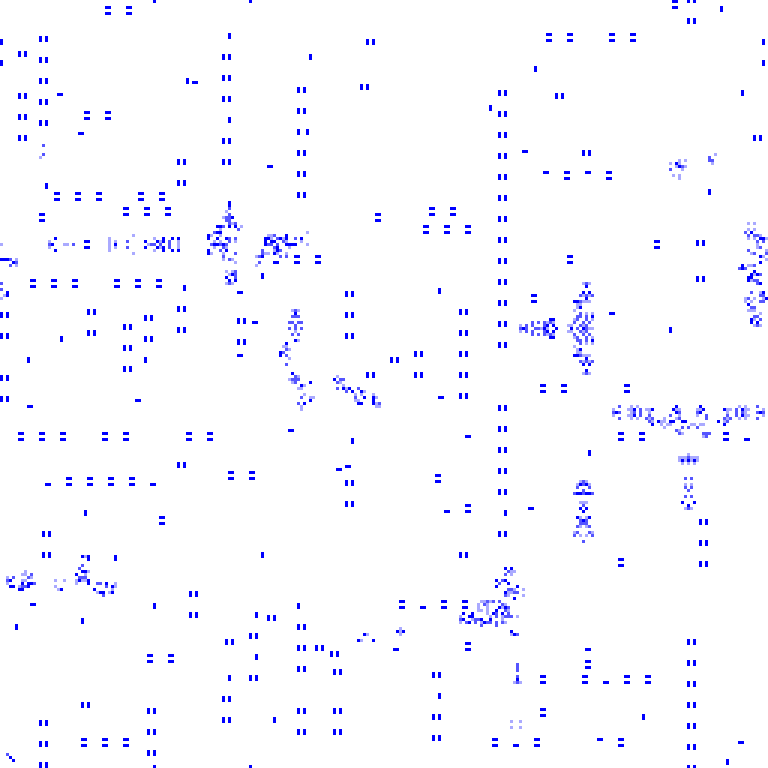
\includegraphics[width=\linewidth]{figures/viz10460682591249143347/base-76.png}}
    \caption{\label{subfig:gol}Base grid}
  \end{subfigure}
  \hfill
  \begin{subfigure}{.48\linewidth}
    \fbox{
    \centering
    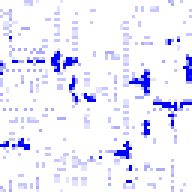
\includegraphics[width=\linewidth]{figures/viz10460682591249143347/coarse-76.png}}
    \caption{\label{subfig:gol_cg}Coarse-grained}
  \end{subfigure}

  \caption{\label{fig:gol_comparison}\textbf{Side-to-side comparison of a CA
      simulation and its coarse-grained version}. The first simulation is $256
    \times 256$ cells and the second has been coarse-grained to $64\times 64$.
    Notice the interesting patterns on Figure~\ref{subfig:gol} are hardly
    distinguishable. They are highlighted by histogram-based coarse-graining in
    Figure~\ref{subfig:gol_cg}.}
\end{figure}


\subsubsection{Hierarchical coarse-graining.}
The above procedure can be applied recursively to the same cellular automaton or
with larger block sizes to get a progressively coarser representation. Since
information is systematically discarded in the process, it cannot be applied any
number of times. For this reason, many 2D CAs exhibiting interesting behaviors at
the micro-level but not at the macro-level have no remaining visible structure
after reducing their scale several times with this method.

Because a simple model like frequency counting can be estimated quickly,
hierarchical coarse-graining is easily applied to large grids, reducing the size
by a factor of $n$ (block size) every time. For instance, this property makes it
suitable to search the cellular automata rule space for CAs behaving
interestingly at multiple coarse-graining levels simultaneously.

\subsection{Clustering}

Another way to convert blocks of cells for coarse-graining is to distribute
these blocks into a small number of clusters, where each group becomes the new
coarse state.

Several distance functions may apply here, the most natural of which being
Hamming distance, which measures how many states differ between two
positions~\parencite{hammingErrorDetectingError1950}. It is defined for two strings
of equal length $n$, $s_1 = [s_{(1, 1)}, \ldots, s_{(1,n)}]$ and $s_2 =
[s_{(2,1)}, \ldots, s_{(2,n)}]$, as the number of positions where the two
strings differ:
\begin{align}
  \sum_{k = 1}^n \mathds{1}\left\{\ s_1^{(k)}  \neq s_2^{(k)}\right\}.
\end{align}

A supercell of $N\times N$ cells of a CA can be converted into a string to be
compared to other blocks with the Hamming distance. For CAs, we limit ourselves
to strings of digits representing states, i.e. $s_{(i,j)} \in \mathbb{N}$. We
use a vanilla implementation of the K-means algorithm where clusters' centers
are computed using a continuous average of position vectors rounded to nearest
integer values. Clusters are initialized with randomly selected observations.

\subsection{Autoencoders for coarse-graining}

Instead of just relying on the amount of information of a given supercell's
configuration, one can also try to automatically find a relevant representation
with dimensionality reduction methods. Autoencoders are neural networks composed
of an encoder part and a decoder part, originally designed to identify principal
components of a collection of data
points~\parencite{baldiNeuralNetworksPrincipal1989,
  hintonConnectionistLearningProcedures1989,
  kramerNonlinearPrincipalComponent1991}. An encoder neural network converts
data to a \emph{latent} vector of smaller dimension than the original input.
Then, a decoder neural network reconstructs a vector with the same dimension as
the input from this encoded \emph{latent} representation.These models can
automatically find an optimal constrained representation through minimizing a
reconstruction loss between the original input and the reconstructed output.

We denote the encoder network with $E$ and the decoder network with $D$. We frame
the reconstruction problem as a $N$ class classification problem with multiple
components --- one class per input state, one component for each cell of the $K$
cells in a block. The reconstruction loss is the component-wise cross-entropy
between the state of each input cell and the reconstructed state after $D \circ
E$ is applied.

\begin{figure}[th]
  \centering
  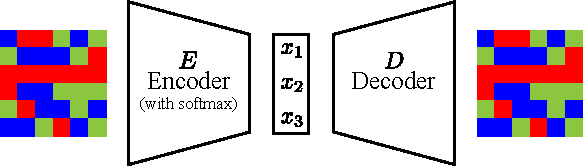
\includegraphics[width=\linewidth]{figures/autoencoder.pdf}
  \caption{\label{fig:autoencoder} \textbf{Diagram of the autoencoder
      architecture used for coarse-graining}. A block of $6\times 6$ cells is
    encoded in a vector of fixed dimension. There are 3 components in the
    example. They can either represent a RGB color or a 3 states smaller
    automaton.}
\end{figure}

Figure~\ref{fig:autoencoder} illustrates the autoencoder layout for
coarse-graining. By adjusting the block size and dimension of the encoded
vector, one can influence the amount of information conserved during encoding.
Naturally, smaller blocks will be more easily represented in lower dimension.

The encoder has a softmax layer to ensure the coded state's components sum to
one. Therefore, one can view this coded supercell as a mixture of states which
can either be kept as is or converted to a discrete state by keeping the maximal
component only. They are trained with stochastic gradient descent until
convergence.

\section{\label{sec:results}Results}

We evaluate our proposed coarse-graining methods in the following two different ways:
\begin{itemize}
\item We compare our results on elementary cellular automata (ECA) to previous
  works on particle and domain filtering.
\item We use a metric which evaluates complexity of CAs introduced
  in~\parencite{cisnerosEvolvingStructuresComplex2019} in order to compare our
  methods' complexity metric scores of the coarse-grained systems and contrast
  the scores against a standard image processing baseline that computes local
  average of neighbouring cells followed by downscaling the grid. Using the
  complexity metric we measure to what extent the interesting behavior of
  cellular automata is conserved after coarse-graining compared to this image
  processing baseline.
\end{itemize}

In the following we begin by showing that a simple histogram-based
coarse-graining is effective at detecting structures (such as gliders) in ECA
space-time diagrams. Our method achieves results comparable with previous work,
while being simpler to apply.

\subsection{Domains and filtering}

In the space-time diagrams of cellular automata, moving structures such as
gliders are embedded in uniform or periodic backgrounds, or ``domains''. This
domain is different depending on the rule: some ECAs have uniform backgrounds,
checkerboard backgrounds or more complicated patterns (e.g.\ rule
110).~\parencite{crutchfieldTurbulentPatternBases1993} also identified chaotic
domains, which cannot support regular gliders but have ``walls'' and
``particles''. Those correspond, respectively, to boundaries between two chaotic
domains and propagating defects (localized structures with a pattern different
from the domain) within a domain.

Our proposed coarse-graining methods offer interesting perspectives to filter
cellular automata's space-time diagrams, which enables identifying gliders and
studying the formation of large-scale patterns. We find that a simple histogram
coarse-graining achieves results comparable to those reported
in~\parencite{hansonAttractorbasinPortraitCellular1992,
  elorantaKinkCellularAutomaton1992, hansonComputationalMechanicsCellular1997,
  wuenscheExploringDiscreteDynamics2011} for ECA rules 18 and 54. A similar
approach was undertaken in \parencite{wuenscheClassifyingCellularAutomata1999} in
which the authors used the entropy of rule table lookup frequencies to filter
out regular domains in the space-time diagrams of cellular automata and to
identify gliders and domain boundaries. However, Wuensche's approach described
in~\parencite{wuenscheClassifyingCellularAutomata1999} does not attempt to downscale
space-time diagrams.

\subsection{Results on elementary cellular automata}

\begin{figure}[th]
  \centering
  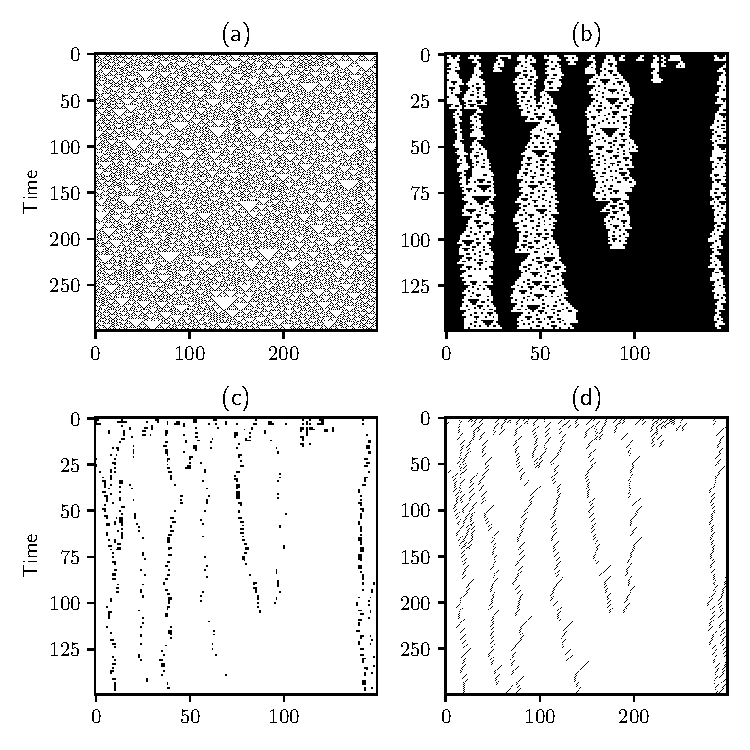
\includegraphics[width=\linewidth]{figures/rule18.pdf}
  \caption{\label{fig:rule18} \textbf{Space-time diagrams for rule 18 in
      elementary cellular automata.} \textbf{(a)} Standard rule 18 space-time
    diagram, starting from a random position. \textbf{(b)} Filtered domain with
    our frequency coarse-graining (even). \textbf{(c)} Our domain boundaries
    extracted from the filtered domains in \textbf{(b)}. \textbf{(d)} Domain
    boundaries computed according to
    \parencite{hansonAttractorbasinPortraitCellular1992}. Note that \textbf{(a)}
    shows semi-chaotic behaviour, which is hard to interpret, whereas our method
    \textbf{(b)} highlights distinct domains within the disordered space-diagram
    in (a). The detected domains and domain boundaries from previous work (d)
    and ours (c) are very similar.}
\end{figure}

We apply frequency histogram-based coarse-graining on elementary cellular
automata (ECA) and obtain space-time diagrams with suppressed background
domains. Resulting partitions of ECAs' space-time diagram are similar to results
reported by~\parencite{hansonAttractorbasinPortraitCellular1992,
  hansonComputationalMechanicsCellular1997}. Figure~\ref{fig:rule18}\textbf{(a)}
and~\ref{fig:rule54}\textbf{(a)} show the space-time diagrams of rules 18 and 54
with random initialization. Boundaries between different background patterns in
both Figures were obtained with coarse-graining; they are similar to boundaries
obtained by Hanson and Crutchfield. We also observe the propagation of many of
the same particles and defects without any prior information about the cellular
automaton rule.

Particles in Rule 54 have been used to implement
computations~\parencite{boccaraParticlelikeStructuresTheir1991,
  pivatoSpectralDomainBoundaries2007,
  martinezCompleteCharacterizationStructure2014}. Because the presented
reduction reduces the size of the grid, it can merge some of those particles,
sometimes resulting in ambiguities and gaps. However, our goal here is not to
precisely describe particle interactions in order to manipulate or construct
complex computations manually. Underlying computations described in the works
above are still happening within our reduced CA simulation. We consider the
\emph{apparent} destruction of some of these fine-scale details acceptable in
order to discover larger-scale complex behavior.

Our method is also arguably much simpler than computational mechanics (used by
Hanson and Crutchfield) which requires some reverse-engineering of the rule and
the construction of a finite-state transducer to generate output symbols.
Although full automation has been demonstrated, this method introduces
significant overhead~\parencite{rupeLocalCausalStates2018}. On the other hand, our
method is sensitive to the quality of statistical estimation of the frequency
histogram (see equation~\eqref{eq:stat_est}) and needs enough input examples to
achieve a reasonable result --- examples in Figure~\ref{fig:rule18}
and~\ref{fig:rule54} used simulations with the width of 3000 cells, ran for 6000
timesteps to obtain reliable pattern frequency estimates.

In the Figures, we used the coarse-graining method introduced
in~\nameref{sec:simple-hier-coarse}. Space-time diagrams are coarse-grained by a
factor 2 to a binary automaton --- each cell corresponds to a 2-cell block.
These binary coarse-graining results in the Figures are labeled \textbf{(c)}.
Because of the statistical nature of the domains of these 1D ECA's and the use of
blocks of size 2, filtered domains differ depending on the starting position of
coarse-graining. We distinguish an odd and even filtered domain.

Figure~\ref{fig:rule18}\textbf{(c)} is obtained by applying the element-wise
\texttt{OR} operator to both the even and odd domain diagrams to merge them into
a single space-time diagram. Figure~\ref{fig:rule54}\textbf{(c)} is obtained by
computing differences between neighboring cells after the filtering process to
highlight lines. Figure~\ref{fig:rule110} is another example showing filtering
of particles in rule 110.


\begin{figure}[th]
  \centering
  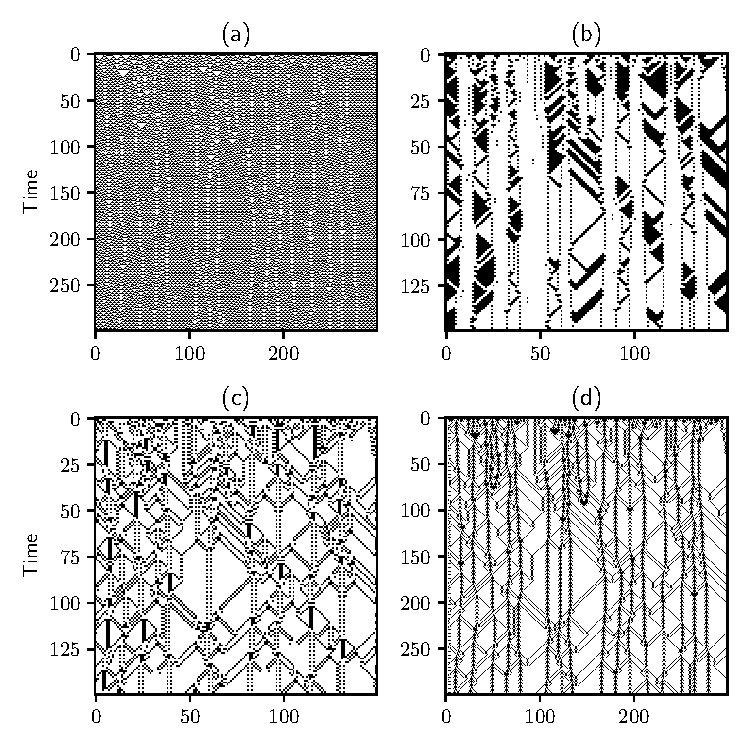
\includegraphics[width=\linewidth]{figures/rule54.pdf}
  \caption{\label{fig:rule54} \textbf{Space-time diagrams for rule 54}.
    \textbf{(a)} Space-time diagram of standard rule 54, starting from a random
    position. \textbf{(b)} Filtered domain with our frequency coarse-graining
    (even). \textbf{(c)} Particles filtered from the domains in \textbf{(b)
      using our method}. \textbf{(d)} Domain boundaries computed using
    computational mechanics \parencite{hansonComputationalMechanicsCellular1997}.
    Please note that particles are detected equally well using computational
    mechanics (d) and our (simpler) frequency-based method (c). Some close-by
    particle trails are merged using our method.}
\end{figure}

\begin{figure}[t]
  \centering
  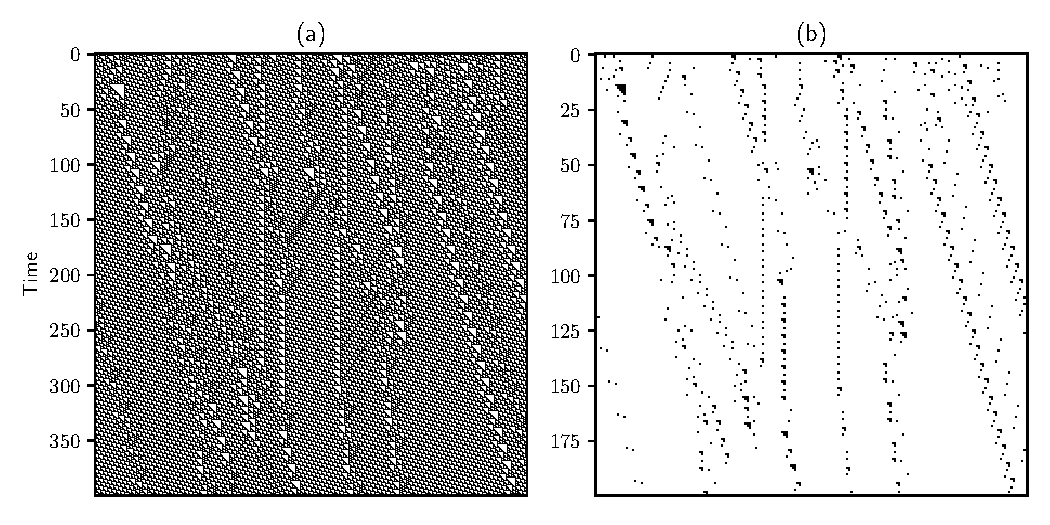
\includegraphics[width=\linewidth]{figures/rule110.pdf}
  \caption{\label{fig:rule110} \textbf{Spate-time diagram of rule 110 (\textbf{a})
      and filtered particles using our histogram-based coarse-graining
      (\textbf{b})}. Structures propagating in time (vertical axis) and space
    (horizontal axis) become clearly visible in \textbf{(b)} as vertical and
    diagonal lines.
    %\textbf{(b)} shows the same structures with the regular
    %background domain filtered out with our method.
    }
\end{figure}
\subsection{Complexity metrics and coarse-graining}

\setlength{\fboxsep}{0pt}
\begin{figure}[th]
  \centering
  \begin{subfigure}{.48\linewidth}
    \fbox{\centering
      
\includegraphics[width=\linewidth]{figures/13220943837485080965/19_rule_downscale_13220943837485080965-20.png}}
    \caption{\label{subfig:downscale3} Downscaling by averaging}
  \end{subfigure}
  \begin{subfigure}{.48\linewidth}
    \fbox{\centering
      \includegraphics[width=\linewidth]{figures/13220943837485080965/19rule_coarsed_13220943837485080965-20.png}}
    \caption{\label{subfig:histogram3} Histogram}
  \end{subfigure}
  \begin{subfigure}{.48\linewidth}
    \fbox{\centering
      \includegraphics[width=\linewidth]{figures/13220943837485080965/19rule_kmeans_13220943837485080965-20.png}}
    \caption{\label{subfig:kmeans3} K-means}
  \end{subfigure}
  \begin{subfigure}{.48\linewidth}
    \fbox{\centering
    \includegraphics[width=\linewidth]
    {figures/13220943837485080965/19rule_autoencoder_13220943837485080965-20.png}}
    \caption{\label{subfig:autoencoder3}Autoencoder}
  \end{subfigure}
  \caption{\label{fig:qualitative}\textbf{Qualitative comparison of
      coarse-graining methods}. Simulations are on grids of $4096 \times 4096$
    cells coarse-grained to $512 \times 512$. Lines are barely visible with
    downscaling~\ref{subfig:downscale3}, but are visible
    in~\ref{subfig:histogram3}-\ref{subfig:autoencoder3}. Coarse-graining helps
    visualize linear structures that would be hard to see otherwise.}
\end{figure}

Coarse-graining is not only useful for detecting gliders and domains in
space-time diagrams, but also as a tool to visualize large CAs. To evaluate the
quality of our proposed coarse-graining methods, we compare complexity scores
computed according to~\parencite{cisnerosEvolvingStructuresComplex2019} for different
coarse-graining methods. This metric was shown to correlate well with a user
study of interesting automata. It uses neural networks to estimate how easy it
is to learn a compressed representation of a CA\@. We also computed the scores on
downscaled CAs as a baseline. Local averaging is used for downscaling, with each
block of $N$ cells being replaced by its average value rounded to the nearest
integer state.

Experiments begin by sampling 3600 cellular automata rules with 3 or 4 states.
We apply the complexity metric on a randomly initialized simulation on a $512
\times 512$ grid of cells. The top 100 rules with the highest complexity scores,
which should correspond to rules with interesting behaviors, are then used for
coarse-graining. We apply coarse-graining on grids of $4096 \times 4096$ cells,
scaling the grid down by a factor of $8$, and compute the complexity metric also
on the reduced grid. Figures reported in Table~\ref{experiments_table-vc} are
percentages of rules still considered interesting (above the selection threshold
for the first step of the process) after coarse-graining. The higher this number
is, the more a method is able to conserve complex and interesting behaviors
after the reduction.

\begin{table}[t!]
  \centering
  \begin{tabular}{ccccc}
    \toprule
       Local-averaging & K-Means & Histogram & Autoencoder\\
     baseline &  & & \\
    \midrule
      19.3\%  & 40.4\% & 82.4\% & 84.2\%\\
    \bottomrule
  \end{tabular}
  \label{experiments_table-vc}
  \caption{\textbf{Experimental results --- Percentage
      of rules classified as interesting after reduction with our 3 proposed
      methods (K-means, Histogram, Autoencoder), compared to a local averaging baseline.}}
\end{table}

Results in Table~\ref{experiments_table-vc} suggest that using our proposed methods
seems largely beneficial for studying complexity in large systems.
% when usual metrics become impractical.
Histogram and autoencoder methods are superior to downscaling using k-means and
local averaging. This could be attributed to the fact that contrary to the
latter two, the histogram and autoencoder both represent well anomalies (rare
events). This is because rare events are explicitly captured and kept by the
histogram method. They also represent useful information that may be kept for
the reconstruction using the autoencoder.

\subsection{Discussion}\label{sec:discussion}

Downscaling by local averaging is not an effective solution to the
coarse-graining problem for several reasons. In particular, it tends to favor
the majority state in a supercell because of the averaging effect. Thin
structures spanning only few cells placed on a uniform background are likely to
disappear after coarse-graining although they may still be relevant with respect
to the large-scale patterns. The histogram-based method explicitly encodes those
more rare events in a supercell, even if their size is relatively small compared
to the supercell size.
%The autoencoder may automatically encode this
%information too because those few cells are more useful to reconstruct the
%initial supercell than the background.

Figure~\ref{fig:qualitative} is a qualitative comparison of coarse-graining
methods. This cellular automaton was selected from the experimental dataset.
When simulated on large grids, it generates large linear structures that are
4-cells wide. These structure disappear after downscaling by averaging because
the background dominates the average. Other methods correctly highlight these
structures when downscaling the grids by a factor of 8. In
Figure~\ref{fig:dynamics_levels}, we show another rule that was selected for its
high complexity score at multiple coarse-graining scales from our dataset. The
CA has significantly different dynamics depending on the chosen scale.
Example~\ref{subfig:single} is a spontaneously occurring stable oscillating
glider with period 3. Large structures emerge from these simple gliders when
observing large grids. The online project page\footnote{\projecturl} shows
animated example for Figure~\ref{fig:dynamics_levels}, emphasizing the advantage
of using coarse-graining for visualization.

A crucial advantage of the frequency histogram method is its speed and ease of
implementation compared to autoencoders. Other than a few hyper-parameters for
partitioning the histogram, no training or tuning is needed to produce the
coarse-grained output.

\begin{figure}[ht]
  \centering
  \begin{subfigure}{.052\linewidth}
    \fbox{\centering
    \includegraphics[width=\linewidth]{figures/viz5413567812493154659/single_glider.png}}
    \caption{\label{subfig:single}}
  \end{subfigure}
  \begin{subfigure}{.45\linewidth}
    \fbox{\centering
    \includegraphics[width=\linewidth]{figures/viz5413567812493154659/mult_glider.png}}
    \caption{\label{subfig:mult_glider} $128 \times 128$ cells}
  \end{subfigure}
  \begin{subfigure}{.45\linewidth}
    \fbox{\centering
    \includegraphics[width=\linewidth]{figures/viz5413567812493154659/mult_glider_larger.png}}
  \caption{\label{subfig:mult_glider_larger} $512 \times 512$ cells}
  \end{subfigure}
  \begin{subfigure}{.48\linewidth}
    \fbox{\centering
      \includegraphics[width=\linewidth]{figures/viz5413567812493154659/waves_b.png}}
    \caption{\label{subfig:waves_b} $2048 \times 2048$ cells coarse-grained to $256 \times 256$.}
  \end{subfigure}
  \hfill
  \begin{subfigure}{.48\linewidth}
    \fbox{\centering
      \includegraphics[width=\linewidth]{figures/viz5413567812493154659/waves_c.png}}
    \caption{\label{subfig:waves_c} $4096 \times 4096$ cells coarse-grained to $256 \times 256$.}
  \end{subfigure}
  \caption{\label{fig:dynamics_levels} \textbf{Changing CA dynamics at multiple
      scales}. (a) shows a single glider, oscillating between 3 positions. Such
    gliders emerge spontaneously from a random initialization of a small grid as
    shown in (b). When scaling the grid up, trails of gliders begin to appear,
    creating moving straight and diagonal lines as shown in (c). Scaling-up even
    more, individual gliders are not visible anymore, as shown in (d). In an
    even larger grid, shown in (e), many more triangular-shaped waves travel and
    collide with each other. Please note that (d) and (e) are coarse-grained to
    $256 \times 256$, otherwise the patterns are not visible.}
\end{figure}


% \begin{figure}[th]
% \begin{subfigure}{.48\linewidth}
%   \centering
%   \includegraphics[width=\linewidth]
%   {figures/3904718678772130032_autoencoder/3904718678772130032_autoencoder-20.png}
%   \caption{\label{fig:autoencoder1}Autoencoder}
% \end{subfigure}
% \begin{subfigure}{.48\linewidth}
%   \centering
%   \includegraphics[width=\linewidth]{figures/3904718678772130032_coarsed/3904718678772130032_coarsed-20.png}
%   \caption{\label{fig:histogram1}Histogram}
% \end{subfigure}
% \end{figure}

% \begin{figure}[th]
%   \begin{subfigure}{.48\linewidth}
%     \centering
%     \includegraphics[width=\linewidth]
%     {figures/18072167875025464602_autoencoder/18072167875025464602_autoencoder-20.png}
%     \caption{\label{fig:autoencoder2}Autoencoder}
%   \end{subfigure}
%   \begin{subfigure}{.48\linewidth}
%     \centering
%     \includegraphics[width=\linewidth]
%     {figures/18072167875025464602_coarsed/18072167875025464602_coarsed-20.png}
%     \caption{\label{fig:histogram2} Histogram}
%   \end{subfigure}
% \end{figure}

\section{Conclusion\label{sec:conclusion-vc}}

We intend to use these coarse-graining methods to find cellular automata (CA) which
exhibit interesting behaviors at multiple scales.
Figure~\ref{fig:dynamics_levels} shows an example of such a CA\@. We observe
various dynamics depending on the scale, from simple oscillating gliders to
large wave-like patterns composed of thousands of gliders. It demonstrates that
observing multi-scale behaviors within those automata is possible. The existence
of 2D cellular automata with disordered behaviors at the smallest level but
organized at coarser scales, similar to hidden patterns in rule 18, would also
be of great interest.

Cellular automata are powerful computational models. Some of them have been
shown to be Turing-complete, and can thus be expected to support arbitrarily
complex computations~\parencite{berlekampWinningWaysYour2001,
  cookUniversalityElementaryCellular2004}. Naturally, most interesting CAs
spontaneously generate a fraction of available computations at a time, usually
supporting a few stable oscillators or moving structures. Proofs of universality
for these CAs required careful design of computational devices out of these
stable oscillators and structures, resulting in very brittle and inefficient
universal computers. In practise, only elementary functions --- such as density
classification, binary addition, etc. --- can be implemented. This requires
searching for CA rules specifically targeted at a particular
function~\parencite{mitchellEvolvingCellularAutomata1996, wolframNewKindScience2002,
  sapinResearchCellularAutomaton2003}. Hierarchies are central to naturally
occurring complex phenomena~\parencite{simonArchitectureComplexity1962}, and may be
required for robust and complex processes to emerge in CAs.

Viewing space-time diagrams of cellular automata is akin to visualizing a
foreign computer design. Cellular automata are manipulating information,
registers and instructions in parallel in the form of cell states. We believe
visualization tools proposed in this paper can help understand computations in
those unconventional computers. By reducing available information to its
essential parts, we attempt to distill the content of the space-time diagram
with as little prior information as possible. Future work could focus on
identifying some known simple computational primitives within cellular automata
and understanding how our visualization can help to find them.

These methods also enable apprehending large grid sizes for which even image
processing algorithms begin to show limitations. Complexity metrics and CA
classification techniques can be extended to these reduced large grids and could
lead to the discovery of CAs with --- similar to life and physical processes ---
significantly different dynamics at multiple scales that could in turn be a
basis for artificial evolution.

\chapter{Learning efficiency of complex systems for reservoir computing}

  It is common to evaluate the performance of a machine learning model by
  measuring its predictive power on a test dataset. This approach favors
  complicated models that can smoothly fit complex functions and generalize well
  from training data points. Although essential components of intelligence,
  speed and data efficiency of this learning process are rarely reported or
  compared between different candidate models. In this paper, we introduce a
  benchmark of increasingly difficult tasks together with a data efficiency
  metric to measure how quickly machine learning models learn from training
  data. We compare the learning speed of some established sequential supervised
  models, such as RNNs, LSTMs, or Transformers, with relatively less known
  alternative models based on reservoir computing. The proposed tasks require a
  wide range of computational primitives, such as memory or the ability to
  compute Boolean functions, to be effectively solved. Surprisingly, we observe
  that reservoir computing systems that rely on dynamically evolving feature
  maps learn faster than fully supervised methods trained with stochastic
  gradient optimization while achieving comparable accuracy scores. The code,
  benchmark, trained models, and results to reproduce our experiments are
  available at {\small\url{https://github.com/hugcis/benchmark_learning_efficiency/}}.


\section{Introduction}
Most machine learning models are evaluated by measuring performance on a
specific dataset or task. Learning efficiency -- the ability to learn,
generalize, and adapt quickly from a few examples -- is crucial for practical
intelligence \cite{kanazawaGeneralIntelligenceDomainspecific2004} as well as
low-data machine learning applications, yet rarely used to evaluate models.
Supervised learning systems are theoretically limited in their learning speed by
the optimization algorithms used for training. These algorithms such as
stochastic gradient descent (SGD) have various speed guarantees depending on the
structure of the function to be
optimized~\cite{bottouOptimizationMethodsLargescale2018}. However, when
intelligent beings learn, they appear to quickly re-use past knowledge and
progressively improve over time. Their learning speed depends on a dynamically
evolving internal state.
To measure the learning efficiency of various systems, in this work, we propose the \ac{WADE}
metric based on the time taken to reach several test accuracy checkpoints. We
also design a simple modular benchmark composed of a set of sequential tasks.
They begin with the task of recognizing a simple periodic sequence in an input
string and end with elaborate question answering tasks that require counting
occurrences of patterns and long-term memory.

Established sequential supervised models such as recurrent neural networks
\cite[RNNs; ][]{elmanFindingStructureTime1990}, long short-term memory networks
\cite[LSTMs;][]{hochreiterLongShortTermMemory1997} or Transformers
\cite{vaswaniAttentionAllYou2017} lack essential properties such as learning
beyond the training phase or the ability to adapt over time after being trained. These models can also be expensive to train, requiring a large number
of labeled training examples to reach reasonable performance, leading to poor
learning speeds. In this work, we use the newly proposed \ac{WADE} metric and the benchmark dataset to experimentally compare the learning speed of these well-established models, such as RNNs, LSTMs and Transformers, with less explored {\em reservoir computing models}.

Reservoir computing is a computational framework that aims to exploit the states
of a complex dynamical system. The simplest example of a reservoir computer is a
\ac{RNN} with frozen weights. This special \ac{RNN} performs random manipulation
on its hidden state in reaction to each new input.
Interestingly, it has been shown that with a
specific initialization of the frozen weights, these \ac{RNN}s (called Echo
state networks) can keep a memory of past inputs
\cite{jaegerEchoStateApproach2001}.
Usually, a standard linear regression is
added as a decoder to extract valuable representation from the hidden state for
some downstream task. Freezing the weights of these recurrent models is useful
when available supervision is very limited or non-existent or for reinforcement
learning with sparse rewards since direct training would be impossible. In such
cases a reservoir computer creates a continuously evolving pool of random
functions that can be combined using the last trainable layer.




When evolving in response to input stimuli, complex recurrent systems such as
\acp{RNN} are building dynamically changing representations of data within their
internal state \cite{boccaraModelingComplexSystems2010}. We know that these
internal states can be interesting on their own because of their ability to
self-organize and exhibit increasingly complex behaviors
\cite{koppelAlmostMachineindependentTheory1991,
  bennettLogicalDepthPhysical1995, allenEvolutionEmergenceLearning2003,
  goldsteinEmergenceComplexSystems2011, cisnerosEvolvingStructuresComplex2019}.
In this paper we wish to investigate whether complex dynamical systems --- in particular RNNs with frozen weights (echo-state networks) \cite{jaegerEchoStateApproach2001} and reservoir cellular automata \cite{yilmazReservoirComputingUsing2014} ---
create representations that allow them to learn faster as measured by our
metric.
\vspace{-8pt}
\paragraph{Contributions.} In this paper, we make the following main contributions: First, we introduce the
\acf{WADE} metric to measure the learning speed of various learning systems and use it to benchmark a few standard models on the IMDB text
classification task \cite{maasLearningWordVectors2011}.
Second, we present a benchmark of language-based tasks of increasing difficulty
to evaluate the learning speed in different conditions. The proposed tasks require a wide range of computational primitives, such as memory or the ability to compute Boolean functions, to be effectively solved.  Third, we study the
learning speed of reservoir computing learning models
and compare them with more standard supervised solutions.
\vspace{-8pt}
\section{Related work}
The \ac{WADE} metric is a generalization of the \emph{Time-to-threshold} metric
\cite{taylorCrossdomainTransferReinforcement2007,
  taylorTransferLearningInterTask2007} introduced for measuring transfer
learning in reinforcement learning contexts. In general, the Time-to-threshold
is simply defined as the number of training steps needed to reach a fixed
threshold performance. However this definition leaves open the choice of
threshold or the definition of a training step. \ac{WADE} alleviates this issue
by aggregating several of these thresholds into a single number that summarizes
the learning speed.

Other metrics for measuring how quickly a model adpats to new tasks have been
introduced in the context of transfer learning, few-shot and zero-shot learning.
In few-shot learning, one tries to obtain the best performance for a particular
task using a small amount of labeled data compared to the task's fully
supervised equivalent~\cite{wangGeneralizingFewExamples2020}. This correlates
with a model's learning speed, but these problems often measure how much prior
information about similar data has been encoded in the models. With our
benchmark and the \ac{WADE} metric, we explicitly measure the number of steps to reach
multiple test accuracy values using all the data needed, effectively emphasizing
data efficiency.

Sample efficiency has also been studied in the context of
reinforcement learning. \cite{chevalier-boisvertBabyaiPlatformStudy2018} use the
number of demonstrations before a task is solved to measure sample efficiency.
This requires defining what solving the task means, which may vary from task to
task. Another approach is to measure performance (cumulated reward, accuracy,
\etc) after a fixed budget of training steps
\cite{yaratsImprovingSampleEfficiency2019}. In this case, the most efficient
model is the one that achieves the best performance within the allocated budget.
In other cases, the sample efficiency is mentioned but not explicitly measured
and one has to examine the learning curves
\cite{buckmanSampleefficientReinforcementLearning2018}. The \ac{WADE} metric is
a general approach to measure the learning efficiency of machine learning
models. We use it to benchmark a few standard models on the IMDB text
classification tasks \cite{maasLearningWordVectors2011} and propose a set of
modular and extensible language based tasks.

Synthetic tasks such as ours have played a vital role in a series of crucial
advances in machine learning algorithms. For example, the XOR problem has
partially motivated the development of neural networks
\cite{minskyPerceptronsIntroductionComputational1972,
  rumelhartLearningInternalRepresentations1985}, and the \emph{circle and ring}
dataset has inspired the creation of novel clustering algorithms
\cite{ngSpectralClusteringAnalysis2001}. The design of synthetic datasets has also been
an essential component of the development of learning algorithms with
memory and general computational capabilities
\cite{hochreiterLongShortTermMemory1997,
  joulinInferringAlgorithmicPatterns2015, gravesNeuralTuringMachines2014,
  westonAICompleteQuestionAnswering2016, richardsonProbingNaturalLanguage2020}.

Other tasks are based on real datasets with artificial manipulations
\cite{krizhevskyLearningMultipleLayers2009, srivastavaCompeteCompute2013a,
  goodfellowEmpiricalInvestigationCatastrophic2014,
  nguyenVariationalContinualLearning2017}. The goal of our dataset is to be
truly progressive in difficulty yet simple to understand and extend, to allow
applications in the field of online learning, and to easily understand a model's
basic computational capacities. Combined with our metric, it enables us to
measure learning speed across a range of conditions. In contrast to similar
synthetic datasets, we built this benchmark so that the last task is vastly more
complicated than the first and could still be extended to more complex examples.




\section{A benchmark for reservoir computing\label{sec:tasks}}
To measure the learning speed of candidate systems and their ability to improve
over time, we propose a performance metric and a standardized set of tasks. We
want to select those systems that quickly and reliably adapt and learn from new inputs.
For this purpose, we introduce the Weighted Average Data Efficiency (WADE)
metric. It aggregates the speed at which a model reaches several test accuracy
checkpoints. We describe the metric in more detail in Section
\ref{sec:performance-metric}.

To reliably compare learning speeds for various systems on a shared foundation,
we also introduce a novel dataset described in Table~\ref{tab:all-tasks}. It is
made up of sequential tasks that begin with straightforward pattern recognition
and progressively increase in complexity to approach the complexity of natural
language and other complex real-world tasks.

We do not focus on the prediction performance of our models, but rather on their
data efficiency --- the number of example sequences they need to learn from before
reaching a target accuracy on a validation set.

\begin{table}[htbp]
  \centering
  \begin{tabular}{cp{.37\linewidth}p{.48\linewidth}}
    \toprule
    \bfseries Task id & \bfseries Name & \bfseries Description \\
    \midrule
    1 & Simple periodic pattern identification & Identify a simple periodic pattern. \\
    \arrayrulecolor{black!20}\specialrule{0.2pt}{.2em}{.4em}
    2 & Harder periodic pattern identification & Identify a periodic pattern with an arithmetically
                            increasing period. \\
    \arrayrulecolor{black}\midrule
    3 & Symbol counting & Count symbols from a sequence. \\
    \arrayrulecolor{black!20}\specialrule{0.2pt}{.2em}{.4em}
    4 & Pattern counting & Count patterns (delimited group of symbols) from a sequence. \\
    \arrayrulecolor{black}\midrule
    5 & Simple question answering & Answer simple YES/NO questions from a single prompt. \\
    \arrayrulecolor{black!20}\specialrule{0.2pt}{.2em}{.4em}
    6 & Harder question answering & Answer simple YES/NO questions from a single prompt
                                    with a more extensive vocabulary. \\
    \arrayrulecolor{black!20}\specialrule{0.2pt}{.2em}{.4em}
    7 & Question answering with world definition & Answer YES/NO questions from a
                                                   sequence of prompts. \\
    \arrayrulecolor{black!20}\specialrule{0.2pt}{.2em}{.4em}
    8 & Question answering with world definition and counting & Answer YES/NO
                                                                and counting questions from a
                                                                sequence of prompts. \\
    \arrayrulecolor{black!20}\specialrule{0.2pt}{.2em}{.4em}
    9 & Adjective question answering & Answer YES/NO and adjective questions from a
                                       sequence of prompts. \\
    \arrayrulecolor{black!20}\specialrule{0.2pt}{.2em}{.4em}
    10 & Adjective question answering and counting & Answer YES/NO, adjective,
                                                     and counting
                                                     questions from a
                                                     sequence of prompts. \\
    \arrayrulecolor{black}\bottomrule
  \end{tabular}
  \caption{General description of all the tasks in the benchmark.}
  \label{tab:all-tasks}
\end{table}
Standard benchmarks and metrics such as those introduced in this paper have
always been essential in advancing various aspects of machine learning. For
example, the LSTM network demonstrated a superior memory capacity on a set of
synthetic tasks designed to challenge the memory of sequential learning systems
\cite{hochreiterLongShortTermMemory1997}. Our goal with this benchmark is to
emphasize measuring learning speed across tasks of varying difficulties with a
range of computational requirements rather than focusing on performance only. We describe the performance metric and the benchmark next.



\subsection{Performance metric\label{sec:performance-metric}}

We introduce the Weighted Average Data Efficiency (WADE) metric as a way to
measure how quickly a model learns, using a weighted average of inverse times
taken to reach various test accuracy \emph{checkpoints} over time.

It is computed for an evenly distributed set of target accuracies $\sA$. They
represent the \emph{checkpoints} at which the speed of learning is estimated.
For example, we may choose $\sA = [0.1, 0.2, 0.3, 0.4, \ldots, 1.]$. The metric is
then calculated as
\begin{equation}
\text{WADE}(\va) = \frac{1}{\sum \alpha} \sum_{\alpha \in \mathbb{A}}\frac{\alpha}{\text{T}(\alpha, \va)},
\label{eq:wade}
\end{equation}
where $\va = (\eva_{0}, \eva_{1}, \ldots, \eva_{n})$ is a sequence of test accuracies achieved by the evaluated system
sampled at different training steps. The quantity $a_{i}$ typically
corresponds to the accuracy reached after seeing $i$ examples, and
$\text{T}(\alpha, \va)$ is the number of steps in the sequence $\va$ needed to reach
an accuracy of $\alpha$. It is defined as
\begin{equation}
  \text{T}(\alpha, \va) = \min\left\{ i \in \{1, \ldots, n, + \infty \}\; |\; a_{i} \geq \alpha \right\}.
\label{eq:tto}
\end{equation}

We also define $\text{T}(\alpha, \va) = +\infty$ if the accuracy value $\alpha$ is never
reached in $\va$. This is equivalent to appending an additional term $\eva_{+\infty}$
to $\va$, always set to the maximum accuracy 1. Note that by construction,
$\text{T}(\alpha, \va)$ is in $[1, + \infty [$.

\begin{figure}[htbp]
  \centering
 \includegraphics[width=.4\linewidth]{figures/metric_tto}
 \caption{Illustration of the calculation of $\text{T}(\cdot, \cdot)$,
   representing the number of training steps (x axis) needed to reach a certain test
   accuracy $\alpha$ (y axis) from a learning curve. In this example,
   $\sA = [0.1, \ldots, 0.8]$ (y axis). $\text{T}(0.6, \va)$ is highlighted in red.
   $\text{T}(0.8, \va) = +\infty$ as the accuracy of 0.8 is never reached.}
  \label{fig:metric_tto}

\end{figure}


Since $\text{T}$ can be $+\infty$ we define
$\frac{1}{+\infty} = 0$ for the quantity in \eqref{eq:wade} to always exist. A visual
intuition of $\text{T}(\cdot, \cdot)$ is given in \figref{fig:metric_tto}.


The choice of checkpoints $\sA$ does not need to be tuned in any specific way
because $\text{WADE}(\va)$ quickly converges to a single value when $\sA$
approaches the continuous interval $[0, 1]$. The approximation is good enough as
long as $\sA$ is not too coarse (more than ten elements was enough in our
experiments) and the WADE values computed from the same set $\sA$ are
comparable.

The time-to-threshold $\text{T}$ is always greater than or equal to 1 step for any threshold and sequence of accuracy scores.
We have
$\forall\: \alpha \in [0, 1],\;  \forall\: \va = (\eva_{n})_{I \subset \{\mathbb{N}\; \cup \{+\infty\} \}}$, and we have
\begin{equation}
  \label{eq:wade-0-1}
\frac{1}{\text{T}(\alpha, \va)} \leq 1,
\end{equation}
and therefore we always get $0 \leq \text{WADE}(\va) \leq 1$. The metric is equal to $0$
for systems that never get past the smallest possible accuracy, while $1$
corresponds to reaching a perfect test accuracy in one single training step. Such
a system would also be considered to be performing well according to the
underlying performance metric with which it is usually evaluated. Therefore,
maximizing WADE also maximizes performance.


\subsection{Description of tasks in the benchmark\label{sec:descr-tasks-benchm}}

This section provides a more detailed description of each task in our benchmark.
The tasks are designed to be language modeling tasks, where the goal is to
predict some tokens from sequences of previously processed tokens. An overview
of the tasks is given in Table~\ref{tab:all-tasks}. The tasks are divided into three
groups: (i) binary tasks with only binary symbols, (ii) general symbolic tasks
-- symbolic manipulations with arbitrary symbols, and (iii) language-based tasks, where symbols represent words in English and behave like a language. We introduce
this benchmark together with the WADE metric, but both can be used in other
contexts as well to measure the learning speed of other systems. Individual
sentences are generated and divided into a training set and a test set for
periodic evaluation of the test accuracy. We give a more detailed description of
each task below\footnote{The tasks are also available as a
  \href{https://github.com/hugcis/incremental_tasks}{Python package on GitHub}.}:

\subsubsection{Binary}
\paragraph{Simple periodic pattern identification.}

The goal of the periodic binary task is to teach the model a fixed-length
regular pattern. As the system is presented with new binary input tokens, it has
to learn the periodic pattern on the fly and correctly predict the next token. A
pattern of size $n$ is chosen at random and repeated $k$ times to produce a
sequence of length $n \times k$. Examples include:
\begin{align*}
  \begin{split}
  \smtt{\textbf{01}01010101010101010101010101010101} & \quad\text{Pattern with period 2}\\
  \smtt{\textbf{0011}001100110011001100110011001100} & \quad\text{Pattern with period 4}\\
  \smtt{\textbf{011}0110110110110110110110110110110} & \quad\text{Pattern with period 3}
\end{split}\label{eq:1}
\end{align*}

\paragraph{Harder periodic pattern identification.}

For this task, we also draw a random binary pattern of size $n$. Each of its
symbols is repeated $k$ times, with $k$ increasing monotonically from 1. A
successful model must learn the pattern on the fly and correctly implement the
arithmetic increase in the size of the period. We set the pattern length to increase by
1 every period in our experiments, but this value can be changed.

\subsubsection{Symbolic counting}

These tasks consist of reading patterns from an input sequence and answering a
simple query about the number of patterns. Unlike previous tasks, these
require implementing a form of addressable memory that can be queried after the prompt has
ended.

\paragraph{Basic symbol counting.}
The first version of the counting task focuses on counting single symbols from
an input sequence. The sequence ends with a \emph{query} for the count of
one of the symbols. The goal is to predict the last token (in bold) of sequences
of the following form:

\begin{align*}
  \underbrace{\smtt{AABBCBABAAB}}_{\text{Input symbols}}
  & \underbrace{\texttt{x}}_{\text{QS}} \texttt{A}
    \underbrace{\textbf{\texttt{5}}}_{\text{Answer}} \\
\end{align*}

The symbol \texttt{x} is the query symbol (QS) that marks the beginning of the
query. In the first example above, the goal is to predict the token \texttt{5}
because the symbol \texttt{A} appears 5 times. As detailed in
Sect.~\ref{sec:compared-methods}, we represent these nonbinary symbols with
one hot encoding, so the numerical nature of some tokens is not encoded a priori.

\paragraph{Pattern counting.}
This aim of this task is to count the number of occurrences of delimited patterns
instead of single symbols. A sequence is still divided between a prompt --- before
\texttt{x} --- and a query --- after \texttt{x}. One has to predict the symbol
coming after each separator symbol (S) \texttt{y} in the query part of the
sentence. For example, sentences are of the form:

\begin{align*}
  &\underbrace{\texttt{AA}}_{\text{Pattern 1}}\underbrace{\texttt{y}}_{\text{S}}
    \underbrace{\texttt{BBC}}_{\text{Pattern 2}}\underbrace{\texttt{y}}_{\text{S}}\underbrace{\texttt{BAB}}_{\text{Pattern 3}}\underbrace{\texttt{y}}_{\text{S}}\underbrace{\texttt{AA}}_{\text{Pattern 4}}\underbrace{\texttt{y}}_{\text{S}}\underbrace{\texttt{B}}_{\text{Pattern 5}}
    \underbrace{\texttt{x}}_{\text{QS}}\underbrace{\texttt{AAy}}_{\text{Query 1}}\underbrace{\texttt{\textbf{2}}}_{\text{Answer 1}}
    \underbrace{\texttt{By}}_{\text{Query 2}}\underbrace{\texttt{\textbf{1}}}_{\text{Answer 2}} \\
\end{align*}

Multiple queries are presented successively, which requires keeping and being
able to retrieve several counts simultaneously. A query is composed of a
pattern, a separator symbol, and the pattern count that the system should
predict.

\subsubsection{Basic language understanding}
To make the tasks progressively more complex, we steer them towards general
language understanding tasks. The tasks described below are generated automatically, but gradually incorporate more complex skills
required for advanced language processing.
The last task is a step towards understanding the general language albeit with a limited vocabulary.

\paragraph{Elementary question answering (QA).}
This task introduces elements of natural language. Each example is composed of a
stated fact and a question about that fact. A sentence is constructed from a few
basic elements:
(i) Names (\eg\texttt{JOHN}, \texttt{JAMES}, \etc),
(ii) Verbs (\eg\texttt{HEAR}, \texttt{SEE}, \etc),
(iii) Answers (\texttt{YES} or \texttt{NO}),
(iv) Additional words and symbols (\texttt{I, DO, NOT, AND, BUT, ?, .}).

A random subset of names is selected, and we generate a random prompt/question
pair from it.
The question is drawn to ensure an equal proportion of
positive and negative answers. For example, sentences may look like this:

\begin{align*}
&  \texttt{I HEAR JOHN AND PAUL .}\texttt{ DO I HEAR PAUL ?} \texttt{\textbf{ YES}}\\
&    \texttt{I SEE JOHN BUT I DO NOT SEE PAUL AND TOM . DO I SEE TOM ? \textbf{NO}}
\end{align*}

The only token to predict is the binary answer \texttt{YES} or \texttt{NO}.

\paragraph{Question answering (QA) with adjectives.}

This task extends the previous task by adding adjectives and modifiers to the
object names. The queries may be about the subject-verb relation or the
subject-adjective relation.

\begin{align*}
  &\texttt{I SEE A SMALL BANANA .}\texttt{ WHAT IS THE SIZE OF THE BANANA I SEE ? } \texttt{\textbf{SMALL}}\\
  &  \texttt{I SEE A LARGE GREEN APPLE BUT I DO NOT SEE A RED APPLE .} \\
  & \quad\quad\texttt{DO I SEE A LARGE APPLE ? \textbf{YES}} \\
  &  \texttt{I SEE A SMALL GREEN APPLE BUT I DO NOT SEE A BANANA .}\\
  &\quad\quad\texttt{WHAT IS THE COLOR OF THE APPLE I SEE ? \textbf{GREEN}}
\end{align*}

Here the task output space is slightly larger because the model may be
predicting \texttt{YES}, \texttt{NO}, \texttt{SMALL}, \texttt{GREEN}, \etc

\paragraph{Question answering (QA) with world definition.}

This task introduces more complex configurations in which the state of the world is
defined in one or more sentences, and an unknown number of questions follow.
This is more akin to a real-world conversation where stored facts should be
remembered longer and accessed on demand.
For example, below we show a generated group of sentences followed by several questions:
\begin{align*}
  &\texttt{I SEE A SMALL BANANA .}\\
  &  \texttt{I SEE A LARGE GREEN APPLE BUT I DO NOT SEE A RED APPLE .} \\
  &  \texttt{I HEAR A SMALL GREEN APPLE BUT I DO NOT SMELL A BANANA .}\\
  &\quad\quad\texttt{WHAT IS THE COLOR OF THE APPLE I SEE ? \textbf{GREEN}}\\
  &\quad\quad\texttt{HOW MANY THINGS DO I SMELL ? \textbf{ONE}}\\
  & \quad\quad\texttt{DO I SEE A LARGE APPLE ? \textbf{YES}}. \\
\end{align*}

The difficulty of each of these tasks can be modulated by changing the size of the
base vocabulary, the length of sequences, or the number of queries. Our particular setting of these parameters will be described in section~\ref{sec:task-gen-params}.

\section{Standard language classification task}

To show the usefulness of measuring \ac{WADE} on standard language
classification tasks, we train various text classifiers on the IMDB dataset and
compare their \ac{WADE} scores with a usual performance metric for
classification: accuracy. This classification task, first proposed by
\cite{maassRealTimeComputingStable2002}, consists of deciding if a movie review
is positive or negative from its text. It contains 25000 training examples and
25000 test examples. The two labels are balanced in both the training and test
set. This dataset is a high dimensional language-based task with a binary
output.

We study five standard models: (i) an Elman recurrent neural network (RNN)
\cite{elmanFindingStructureTime1990} with $\tanh$ activation functions trained
with backpropagation through time. (ii) A long-short term memory (LSTM)
recurrent neural network \cite{hochreiterLongShortTermMemory1997}, also trained
with backpropagation through time. (iii) A gated recurrent unit (GRU) recurrent
neural network \cite{choPropertiesNeuralMachine2014}. (iv) A standard
encoder-only transformer neural network model \cite{vaswaniAttentionAllYou2017}.
(v) A logistic regression using a bag-of-words representation of each sentence
as input features. All the models are trained with batches of training data
using the Adam optimization algorithm \cite{kingmaAdamMethodStochastic2015}.
Each model's hyperparameters are chosen to ensure they have a similar number of
trainable parameters except for the logistic regression whose parameter count is
solely determined by the input and output dimensions.

  \begin{tabular}{c|cc}
\toprule
& \bfseries WADE $\times 10^{-2}$ (std.) $\uparrow$ & \bfseries Max test accuracy (std.) $\uparrow$ \\
\midrule
    RNN & 1.028 ${\scriptstyle \pm0.283}$ & 0.705 ${\scriptstyle \pm0.076 }$ \\
LSTM & 2.280 ${\scriptstyle \pm0.303}$ & 0.902 ${\scriptstyle \pm0.002 }$ \\
GRU & 2.711 ${\scriptstyle \pm0.318}$ & \bfseries 0.904 ${\scriptstyle \pm0.002 }$ \\
Linear & 3.737 ${\scriptstyle \pm0.745}$ & 0.862 ${\scriptstyle \pm0.000 }$ \\
Transformer & \bfseries 8.716 ${\scriptstyle \pm0.720}$ & 0.872 ${\scriptstyle \pm0.003 }$ \\

    \bottomrule
  \end{tabular}
  \captionof{table}{Comparison of our new WADE metric to assess learning speed and the standard maximum test accuracy on the IMDB
    classification dataset. Results are averaged over 50 separate runs. ($\uparrow$
    indicates that higher is better).
    \label{tab:comp-sup-acc}}

  \begin{figure}

  \centering
  \includegraphics[width=.4\linewidth]{figures/wade_supervised_fixed.pdf}
  \caption{Test accuracy curves for each model. Shaded areas are
    $\pm 1\sigma$ around the average over 50 runs.\label{fig:wade-sup}}%
  \end{figure}

Table~\Ref{tab:comp-sup-acc} shows the results of all models on the IMDB dataset
reporting both the standard test accuracy as well as our new WADE metric
measuring the learning speed of the different models. We report the maximum test
accuracy observed during training. This corresponds to the model checkpoint that
would be selected with a validation set before using it on test data. The
transformer model learns the fastest of all, as shown by its higher WADE score,
but it does not reach test accuracy values as high as the GRU and LSTM model. We
think that this could be attributed to the transformer model over-fitting on the
available data as discussed below.

According to the WADE metric, the RNN is the worst (i.e., slowest to learn) model
with a score of $1.04 \times 10^{-2}$ whereas the linear model and the transformer
are the fastest with a score above $8 \times 10^{-2}$. The transformer seems to have
more reliable learning speeds than the linear model as shown by the lower
standard deviation ($0.7\times 10 ^{-2}$ versus $4.3 \times 10^{-2}$). The LSTM and GRU
models have intermediate and stable learning speeds.
%You can clearly see on the graph why the GRU has slightly better score than the LSTM, with the former's curve being slightly above the latter's.
The GRU has slightly better WADE score than the LSTM, which can be also seen by inspecting the learning curves in figure~\ref{fig:wade-sup} where the GRU is consistently above the LSTM.

However, when we look at the maximum test accuracy we obtain a different ordering,
with LSTM and GRU performing best with slightly above $90\%$ accuracy followed by the
transformer and the linear model (around $86\%$) and finally the RNN with the lowest
accuracy. The LSTM, GRU and linear models all seem to have converged at the end
of the experiment. The transformer's lower final accuracy despite it being
considered a state of the art model may be explained by over-fitting (apparent
on the graph with the test accuracy score going down). Moreover, the RNN clearly
hasn't converged at the end of the experiment which also explains the relatively
low max accuracy score.

Our new WADE metric gives a complementary view of a model's abilities, which may be significantly different from what can be obtained from the usual
performance metrics focused on the final accuracy of the model.


\section{New benchmark: compared methods\label{sec:compared-methods}}

In the following sections, we carry out experiments to measure \acf{WADE} on
the benchmark described in Table~\ref{tab:all-tasks} and introduced in section~\ref{sec:descr-tasks-benchm}. We compare several
baseline models to understand their learning efficiency: three of the most common
sequential machine learning models for which all parameters are trained --- RNNs, LSTMs, and transformes --- with two methods using reservoir computing: the echo-state networks
(ESN, with a random RNN reservoir) and reservoir cellular automata (ReCA, with a
cellular automaton reservoir) for which only a fraction of the parameters are
learned. Table~\ref{tab:methods-summary} presents all the methods we study in
our experiments.
\begin{table}[h]
  \centering
  \begin{tabular}{lll}
    \toprule
    \multicolumn{2}{l}{\bfseries Methods} & \bfseries Type \\
    \midrule
   RNN & Recurrent neural networks  & \multirow{3}{*}{Fully trained}\\
   LSTM & Long-short term memory networks  & \\
   Transformer &  & \\
    \midrule
   ESN & Echo-state networks  & \multirow{2}{*}{Reservoir-based}\\
   ReCA & Reservoir Cellular Automata  & \\
    \bottomrule
  \end{tabular}
  \caption{Summary of the compared models: three are fully trained, and two are
    reservoir-based.}
\label{tab:methods-summary}
\end{table}

In all our tasks, the input data is assumed to be categorical and sequential.
Tokens are observed one by one in sequence, we define this input as
$X = [X_{1}, \ldots, X_{t}, \ldots],\; t\in \mathbb{N}, \; \forall t \ X_{t} \in \mathcal{X} \subset \mathbb{N}$, where $t$ is the
time index of the sequence, each $X_{i}$ is a token corresponding to time index
$i$, and $\mathcal{X}$ is the set of numbered input categories --- or different tokens in the
vocabulary. First, each categorical input vector is one-hot encoded into a
vector of size $L$, where $L = |\mathcal{X}|$ is the size of the input vocabulary. We define
$\vx_{t}$ as the encoded vector form of $X_{t}$, and we have
$\forall t,\; \vx_{t} \in {\{0, 1\}}^{L}$, with $\sum_{i = 1}^{L}{(\vx_{t})}_{i} = 1$.
Since the tasks are designed to be generally compatible with language modeling,
the input and output vocabularies are the same.

\subsection{Fully trained sequential models (RNN, LSTM and Transformer)}
We first study two standard supervised recurrent models: (i) an Elman recurrent
neural network (RNN) \cite{elmanFindingStructureTime1990} with $\tanh$
activation functions trained with backpropagation through time. (ii) A
long-short term memory (LSTM) recurrent neural network
\cite{hochreiterLongShortTermMemory1997}, also trained with backpropagation
through time. (iii) An encoder-only transformer model with positional encoding
\cite{vaswaniAttentionAllYou2017}.

The three models are trained with a batched Adam optimization algorithm
\cite{kingmaAdamMethodStochastic2015} to minimize a cross-entropy loss function
between the predicted and target tokens. No other training device, such as
dropout, regularization, or normalization, is used for these fully trained baselines.

\subsection{Echo-state networks and reservoir cellular automata\label{sec:echo-state-networks}}

We use %the notation and
names adapted from \cite{jaegerLongShortTermMemory2012} in
this section. An echo-state network is a random recurrent neural network with
frozen weights and skip-connections. Its random weights are sampled in a
specific way so that it performs random combinations of input vectors with its
current state while keeping a history of past inputs \cite{jaegerEchoStateApproach2001}.


% \subsection{Reservoir cellular automata}
Reservoir cellular automaton (ReCA) is a model similar to echo-state networks
% (described in Section~\ref{sec:echo-state-networks})
but where a cellular automaton (CA) replaces the random RNN. The cellular
automaton can be seen as a \ac{RNN} with additional weigth-sharing similar to
convolutional neural network. The special structure of a recurrent CA update
makes it more likely than random RNNs to generate complex structures
\cite{wolframStatisticalMechanicsCellular1983, wolframNewKindScience2002}.
% A CA can also be seen as a special RNN with a large amount of parameter sharing.
Because CAs were not designed to make use of inputs or produce outputs, we
extend the model to make it accept input vectors and to make reading from the CA
state possible (details in Section~\ref{sec:app-ca-res}).

\subsection{Experimental set-up}
We ran 100 separate experiments with different random seeds for each of the CA
rules, the RNN, LSTM, Transformer, and ESN on each task in the benchmark. These experiments
have a separate input projection matrix for the CA, different random weights
for the ESN, and different weight initialization for the supervised baselines.
The task inputs are also generated from a new seed for every experiment, but
we reuse the seeds for the same experiment on different models to ensure they
were trained with the same data. Intervals of one standard deviation for these multiple
experiments are reported in the result graphs.
%as shaded areas around the curve in Figure~\ref{fig:all_metrics}.
The code to reproduce our experiments is
available on GitHub\footnote{\url{https://github.com/hugcis/benchmark_learning_efficiency}}.


\subsubsection{Training parameters}
For each experiment, we generate 1200 random examples from the task generator.
We split this set randomly into a training set with 80\% of the data --- 960
examples --- and a test set with the remaining 240 examples. The reservoir is run
on each training example for the reservoir-based models, which creates the
input features for training the decoder. The sequential supervised models use
batches of single sequences with the Adam algorithm
\cite{kingmaAdamMethodStochastic2015}. They are trained for ten epochs in total. With
reservoir models, only the last linear layer (the decoder) is trained. We minimize the
cross-entropy loss with stochastic gradient descent (SGD), doing only a single
pass over the 960 training examples.

Every few training steps, we generate the output predictions on the testing set,
decode it, and compute the test accuracy for our WADE metric. Supervision is only
applied on tokens that can be predicted --- similar to masked language modeling,
\eg only the answer token is used in the symbol counting or question answering
tasks. Accuracy is also computed for these symbols only.

\section{Results}

We report the final weighted average data efficiency (WADE) scores on our
benchmark in Table \ref{tab:summary} and accuracy results for comparison in Table~\ref{tab:accuracy_all}. We include the best
elementary reservoir cellular automaton (ReCA) and echo
state network (ESN) with the same internal state size for each task.

\begin{table}[htbp]
  \centering
    \begin{tabular}{lcc|ccc|c}
      \toprule
      \multirow{2}{*}{\bfseries Task ID - Name} & \multicolumn{2}{c|}{Reservoir} &
        \multicolumn{3}{c|}{Fully supervised} & \multirow{2}{*}{\bfseries \shortstack{Human \\ expert}}\\
& \bfseries ReCA & \bfseries ESN & \bfseries RNN & \bfseries LSTM & \bfseries Transformer &  \\
\midrule

\bfseries 1 - Periodic & \bfseries 0.78 ${\scriptscriptstyle \pm0.05 }$ &  0.74 ${\scriptscriptstyle \pm0.05 }$ &  0.31 ${\scriptscriptstyle \pm0.06 }$ &  0.28 ${\scriptscriptstyle \pm0.07 }$  &  0.31 ${\scriptscriptstyle \pm0.04 }$& 1.00 \\
\bfseries 2 - Incremental periodic &  0.57 ${\scriptscriptstyle \pm0.02 }$ & \bfseries 0.72 ${\scriptscriptstyle \pm0.02 }$ &  0.42 ${\scriptscriptstyle \pm0.16 }$ &  0.32 ${\scriptscriptstyle \pm0.11 }$  &  0.49 ${\scriptscriptstyle \pm0.15 }$& 1.00 \\
\bfseries 3 - Symbol counting & \bfseries 0.06 ${\scriptscriptstyle \pm0.01 }$ &  0.04 ${\scriptscriptstyle \pm0.01 }$ &  0.05 ${\scriptscriptstyle \pm0.02 }$ &  0.04 ${\scriptscriptstyle \pm0.02 }$  &  0.03 ${\scriptscriptstyle \pm0.01 }$& 0.11 \\
\bfseries 4 - Pattern counting &  0.12 ${\scriptscriptstyle \pm0.04 }$ & \bfseries 0.14 ${\scriptscriptstyle \pm0.03 }$ &  0.13 ${\scriptscriptstyle \pm0.04 }$ &  0.10 ${\scriptscriptstyle \pm0.05 }$  &  0.08 ${\scriptscriptstyle \pm0.03 }$& 0.09 \\
\bfseries 5 - Basic question answering (QA) & \bfseries 0.31 ${\scriptscriptstyle \pm0.08 }$ &  0.26 ${\scriptscriptstyle \pm0.03 }$ &  0.20 ${\scriptscriptstyle \pm0.06 }$ &  0.17 ${\scriptscriptstyle \pm0.08 }$  &  0.16 ${\scriptscriptstyle \pm0.07 }$& 0.15 \\
\bfseries 6 - Harder QA & \bfseries 0.35 ${\scriptscriptstyle \pm0.11 }$ &  0.26 ${\scriptscriptstyle \pm0.03 }$ &  0.24 ${\scriptscriptstyle \pm0.05 }$ &  0.16 ${\scriptscriptstyle \pm0.07 }$  &  0.12 ${\scriptscriptstyle \pm0.06 }$& 0.12 \\
\bfseries 7 - QA with world def. & \bfseries 0.32 ${\scriptscriptstyle \pm0.10 }$ &  0.27 ${\scriptscriptstyle \pm0.04 }$ &  0.24 ${\scriptscriptstyle \pm0.05 }$ &  0.17 ${\scriptscriptstyle \pm0.07 }$  &  0.11 ${\scriptscriptstyle \pm0.06 }$& --- \\
\bfseries 8 - QA with world def. \& counting &  0.09 ${\scriptscriptstyle \pm0.03 }$ & \bfseries 0.14 ${\scriptscriptstyle \pm0.06 }$ &  0.10 ${\scriptscriptstyle \pm0.05 }$ &  0.05 ${\scriptscriptstyle \pm0.02 }$  &  0.02 ${\scriptscriptstyle \pm0.01 }$& --- \\
\bfseries 9 - Adjective QA &  0.04 ${\scriptscriptstyle \pm0.03 }$ &  0.04 ${\scriptscriptstyle \pm0.04 }$ & \bfseries 0.05 ${\scriptscriptstyle \pm0.03 }$ &  0.03 ${\scriptscriptstyle \pm0.02 }$  &  0.02 ${\scriptscriptstyle \pm0.01 }$& --- \\
\bfseries 10 - Adjective QA \& counting &  0.04 ${\scriptscriptstyle \pm0.02 }$ & \bfseries 0.06 ${\scriptscriptstyle \pm0.02 }$ &  0.05 ${\scriptscriptstyle \pm0.02 }$ &  0.03 ${\scriptscriptstyle \pm0.02 }$  &  0.01 ${\scriptscriptstyle \pm0.01 }$& --- \\
      \bottomrule
    \end{tabular}
    \caption{Comparison of WADE scores (also shown in parentheses in the legend
      in figure~\ref{fig:all_metrics}, higher is better) of the best cellular
      automaton rules (\textbf{ReCA}, \cite{yilmazReservoirComputingUsing2014}) for each task against an echo-state
      network (\textbf{ESN}, \cite{jaegerEchoStateApproach2001}), a \textbf{RNN}, a \textbf{LSTM} \cite{hochreiterLongShortTermMemory1997}, and a
      \textbf{Transformer} \cite{vaswaniAttentionAllYou2017} with the same number of parameters.
      %as the cellular automaton reservoir.
      The dash ``---'' indicates that the task was too
      difficult to complete from memory alone for the human
      expert. Accuracy scores are also reported in Table \ref{tab:accuracy_all}.}\label{tab:summary}
\end{table}
Figure \ref{fig:all_metrics} shows the learning curves for the best reservoir cellular
automaton, as well as the echo-state network, recurrent neural network (RNNs), LSTM, and Transformer
on all ten tasks. Interestingly, the reservoir based-models are consistently more efficient
learners than the fully supervised methods, reaching better accuracy in much
fewer training steps. For example, for tasks 5, 6, and 7, the LSTM needs ten
times more steps to approach the accuracy the reservoir CA model reached in less
than 1000 training steps.

Echo-state networks (ESN) and reservoir cellular automata (ReCA) appear to learn at similar
rates, with no clear advantage for one or the other as each model outperforms
the other on five tasks out of ten. On tasks 2, 4, 8, and 10 the ESN is visibly
faster than the ReCA (see curves Figure \ref{fig:all_metrics}), which explains
the ESN's higher WADE scores even though ReCA reaches higher accuracy values
after several more training steps.

\begin{table}[htbp]
  \centering
    \begin{tabular}{lcc|ccc}
      \toprule
      \multirow{2}{*}{\bfseries Task ID - Name} & \multicolumn{2}{c|}{Reservoir} &
        \multicolumn{3}{c}{Fully supervised} \\
& \bfseries ReCA & \bfseries ESN & \bfseries RNN & \bfseries LSTM & \bfseries Transformer  \\
\midrule
\bfseries 1 - Periodic & 0.99 ${\scriptscriptstyle \pm 0.01}$ & \bfseries 1.00 ${\scriptscriptstyle \pm 0.01}$ & 0.79 ${\scriptscriptstyle \pm 0.08}$ & 0.68 ${\scriptscriptstyle \pm 0.04}$ & 0.69 ${\scriptscriptstyle \pm 0.04}$  \\
\bfseries 2 - Incremental periodic & 0.88 ${\scriptscriptstyle \pm 0.01}$ & 0.87 ${\scriptscriptstyle \pm 0.03}$ & 0.87 ${\scriptscriptstyle \pm 0.00}$ & \bfseries 0.89 ${\scriptscriptstyle \pm 0.02}$ & 0.88 ${\scriptscriptstyle \pm 0.00}$  \\
\bfseries 3 - Symbol counting & 0.80 ${\scriptscriptstyle \pm 0.02}$ & 0.30 ${\scriptscriptstyle \pm 0.02}$ & 0.33 ${\scriptscriptstyle \pm 0.03}$ & 0.36 ${\scriptscriptstyle \pm 0.03}$ & \bfseries 0.97 ${\scriptscriptstyle \pm 0.01}$  \\
\bfseries 4 - Pattern counting & 0.56 ${\scriptscriptstyle \pm 0.01}$ & 0.59 ${\scriptscriptstyle \pm 0.02}$ & 0.61 ${\scriptscriptstyle \pm 0.05}$ & \bfseries 0.61 ${\scriptscriptstyle \pm 0.02}$ & 0.54 ${\scriptscriptstyle \pm 0.03}$  \\
\bfseries 5 - Basic QA & 0.81 ${\scriptscriptstyle \pm 0.03}$ & 0.73 ${\scriptscriptstyle \pm 0.03}$ & 0.51 ${\scriptscriptstyle \pm 0.02}$ & 0.75 ${\scriptscriptstyle \pm 0.05}$ & \bfseries 1.00 ${\scriptscriptstyle \pm 0.00}$  \\
\bfseries 6 - Harder QA & 0.72 ${\scriptscriptstyle \pm 0.04}$ & 0.57 ${\scriptscriptstyle \pm 0.03}$ & 0.51 ${\scriptscriptstyle \pm 0.03}$ & 0.68 ${\scriptscriptstyle \pm 0.07}$ & \bfseries 1.00 ${\scriptscriptstyle \pm 0.00}$  \\
\bfseries 7 - QA with world def. & 0.66 ${\scriptscriptstyle \pm 0.03}$ & 0.60 ${\scriptscriptstyle \pm 0.03}$ & 0.51 ${\scriptscriptstyle \pm 0.04}$ & 0.64 ${\scriptscriptstyle \pm 0.07}$ & \bfseries 1.00 ${\scriptscriptstyle \pm 0.00}$  \\
\bfseries 8 - QA with world def. \& counting & 0.59 ${\scriptscriptstyle \pm 0.03}$ & 0.56 ${\scriptscriptstyle \pm 0.03}$ & 0.47 ${\scriptscriptstyle \pm 0.05}$ & 0.50 ${\scriptscriptstyle \pm 0.06}$ & \bfseries 0.98 ${\scriptscriptstyle \pm 0.01}$  \\
\bfseries 9 - Adjective QA & 0.62 ${\scriptscriptstyle \pm 0.04}$ & 0.49 ${\scriptscriptstyle \pm 0.03}$ & 0.43 ${\scriptscriptstyle \pm 0.04}$ & 0.44 ${\scriptscriptstyle \pm 0.03}$ & \bfseries 0.87 ${\scriptscriptstyle \pm 0.11}$  \\
\bfseries 10 - Adjective QA \& counting & 0.54 ${\scriptscriptstyle \pm 0.02}$ & 0.46 ${\scriptscriptstyle \pm 0.03}$ & 0.47 ${\scriptscriptstyle \pm 0.04}$ & 0.49 ${\scriptscriptstyle \pm 0.03}$ & \bfseries 0.57 ${\scriptscriptstyle \pm 0.04}$  \\


      \bottomrule
    \end{tabular}
    \caption{Comparison of accuracy scores (higher is better) of the
      \textbf{ReCA}, \textbf{ESN}, \textbf{RNN}, \textbf{LSTM}, and
      \textbf{Transformer} models with a similar number of parameters. In contrast to the
      results of table~\ref{tab:summary}, the fully-supervised models are more
      performant when we measure the accuracy, as shown here, but do not necessarily do as well when we measure  the speed of learning, as shown in table~\ref{tab:summary}.
    }\label{tab:accuracy_all}
\end{table}


Even if they lack slightly in accuracy, as seen for example on the curves of task 4,
the two reservoir-based methods consistently outperform the fully supervised
sequential methods (RNNs and LSTMs) in terms of learning speeds. This better
learning efficiency could be explained by the internal state structure
introduced by the CA rules and the special form of the ESN random matrix which
favors memory retention whereas usual recurrent network initialization does not
--- we initialize the weights of the full trained models from a uniform
distribution $\mathcal{U}( - \sqrt{h^{-1}} ,\sqrt{h^{-1}})$ in our experiments, where $h$
is the hidden size.

The human expert scores are estimated based on the authors' performance on
obfuscated versions of the tasks --- all input tokens are mapped to random
symbols. These scores may appear surprisingly low in some of these experiments.
Although the task examples presented in Section~\ref{sec:descr-tasks-benchm}
seem easy to understand, we rely heavily on our prior knowledge about the
symbols to understand the patterns --- the words in tasks 5--10 or the numbers in
tasks 3 and 4. These symbols are randomly remapped in our human experiments, and
more examples as well as a good memory are needed to understand the tasks and
learn the mapping itself, hence the slower learning.

\begin{figure}[htbp]
  \centering
  \includegraphics[width=.96\linewidth]{figures/all_metrics_new.pdf}
  \caption{Average learning curves and WADE scores (shown in parentheses in the
    legend) for each task in the benchmark. The dark blue curves represent the
    best elementary cellular automata (CA) rule and the green curves represent
    the echo-state networks (ESN). Note that the x-axis is logarithmic, showing
    ten times more training steps for the RNN and LSTM. Shaded areas represent
    one standard deviation around the average over the 100 different
    experiments.}
  \label{fig:all_metrics}
\end{figure}

It is interesting to note that RNNs also seem to perform better than LSTMs and
Transformers at the beginning of the training in all tasks but the first two.
Even though the Transformer is nowadays generally considered a superior model,
vanilla RNNs may still remain competitive in the very low data and computation
regimes. This is especially pronounced for tasks 8, 9, and 10, where the RNN
test accuracy curve starts increasing significantly 1000 steps before the LSTM.
After several epochs, the Transformer still outperforms other alternatives in
terms of test accuracy on most tasks.
%limitations

We note that we implicitly assume a fixed cost per training iteration in our
experiments and that each training example is seen once. Without these
requirements, one could achieve higher WADE results at the cost of additional
computations and memory usage by using \emph{replay}-inspired methods
\cite{hintonUsingFastWeights1987, robinsCatastrophicForgettingNeural1993a,
  gepperthBioInspiredIncrementalLearning2016,
  rebuffiIcarlIncrementalClassifier2017} that retrain the models with past
stored inputs. The results in Table~\ref{tab:summary} used each input sequence
once.

\section{Human performance evaluation}
\label{sec:human}
The proposed benchmark is relatively simple to understand and hence one may ask what would be the human performance and what WADE values this would correspond to. In
particular, the language tasks appear to be readily solvable just from one's
understanding of the English language. However, similar to how words are encoded
as vectors before being processed by a neural network, we need to remove any
language-based prior to make the comparison with human performance fair. This
could be achieved in a number of ways. For example, if we map all the available
tokens to random letters of the alphabet the apparently trivial task
{\small \begin{align*}
          & \texttt{I DO NOT SEE PAUL . DO I SEE PAUL ? NO} \\
          & \texttt{I HEAR JAMES BUT I DO NOT HEAR PAUL AND JOHN . DO I HEAR JAMES ? YES}
\end{align*}}

would become significantly less obvious to humans
{\small
\begin{align*}
  & \texttt{w K k A D r K w A D l W} \\
  & \texttt{w Z t g w K k Z D G C r K w Z t l H}.
\end{align*}
}

One would need to read through several of these sentences to identify patterns
such as the fact that \texttt{W} and \texttt{H} represent Yes or No or that
\texttt{r} plays the role of a full stop.

We apply the following procedure in our human evaluation experiments:
\begin{enumerate}
  \item Choose a random task among 10.
  \item Apply a random mapping from the task token to letters of the alphabet.
  \item Present the sequences one by one with the tokens to be predicted hidden.
  \item The user enters his predicted answer.
  \item The valid sequence is shown so the user can learn from their mistakes.
  \item Step 3-5 are repeated until 10 sequences are correctly solved in a row.
  Then we go back to step 2 with a new task.
\end{enumerate}
We add the requirement that no external device such as pen and paper or
note-taking program should be used during the experiment so the user relies
solely on their memory. The accuracy is computed by counting the number of right
answers in a row. For example, three right answers in a row would correspond to an
accuracy of 30\%, while ten right answers in a row is 100\% which also
corresponds to a switch of a task. This accuracy score is attributed to the first
correct answer of the series of correct answers. This means that a series of five correct answers starting from question 6 until question 11 will correspond to reaching the accuracy of 50\% on question 6.
This ensures that ten correct answers on the
first attempt will yield a WADE score of 1.

\section{Experimental parameters}
\label{sec:parameters}
We report all the parameters used in our experiments in table \ref{tab:appendix-params}:
\begin{table}[htbp]
  \centering
  \begin{tabular}{lp{.2\linewidth}p{.35\linewidth}}
    \toprule
    & \bfseries Reservoir-based & \bfseries Fully trained \\
    \midrule
    \bfseries Total number of sequences per task & 1200 & 1200 \\
    \bfseries Number of training sequences & 960 & 960 \\
    \bfseries Number of testing sequences & 240 & 240 \\
    \bfseries Passes over the data (epochs) & 1 & 10 \\
    \bfseries Random runs per task & 100 & 100\\
    \bfseries Algorithm & SGD & Adam \citep{kingmaAdamMethodStochastic2015}\\
    \bfseries Learning rate & $0.001$ & $0.001$ \\
    \bfseries Regularization & weight decay $0.001$ & None \\
    \bfseries Internal state (hidden) size & $1800$ & $h$ task-dependent \\
    \bfseries Number of trainable parameters & $1800 \times \text{dictionary\_size}$ &
      $h^{2} + 2 \times h \times \text{dictionary\_size}$ for the RNN\textsuperscript{2}\\
    \bfseries Output non-linearity & Softmax & Softmax \\
    \bfseries Internal non-linearity & Not applicable & $\tanh$ \\
    \bfseries Batch size  & 1 & 1 \\
    \bottomrule
  \end{tabular}
  \caption{Experimental parameters common to all tasks. Some of the sizes (such
    as $h$) vary from task to task.}
  \label{tab:appendix-params}
\end{table}

\subsection{Task generation parameters\label{sec:task-gen-params}}
The tasks are generated according to the procedures described in
Section~\ref{sec:tasks}. They have some parameters that allow the
difficulty of the task to be adjusted. We report results on ten tasks. The parameters
chosen for our experiments are listed below:
\vspace{-8pt}
\begin{description}
  \item[Periodic (1) and Increasing period (2):] Sequences are generated from patterns of
        length between 1 and 10.
  \item[Easy symbol counting (3):] Available symbols are \texttt{A}, \texttt{B} and
        \texttt{C}. Generated sequences have between 1 and 10 of these symbols
        in the prompt, and the query has either one, two, or all three symbols.
  \item[Hard symbol counting (4):] Available symbols are the same as for the previous
        task. Generated sequences have between 1 and 45 symbols
        with separators in the prompt. There is a minimum of 1 query, and can be
        as many queries as there are different patterns in the prompt.
  \item[Question answering (5):] There are five available names and two verbs. The
        prompt consists of between one and five names, and the question is about one
        of these names.
  \item[Harder question answering :] There are eleven available names and five
        verbs. The prompt is made of between one and five names, and the
        question is about one of these names.
  \item[Question answering with world (7), with counting (8):] There are thirteen available
        names and seven verbs.
  \item[Adjective question answering (9), with counting (10):] There are eight
        available names, six verbs, four color adjectives, and five size
        adjectives. The prompt consists of between one and six statements, and
        there are up to eight questions.
\end{description}

\vspace{-8pt}
We chose relatively small values of these parameters because we are interested in simple tasks
so that models that can learn from less than 100 examples. Moreover, the
number of possible sentences generated from these small values is already huge,
with more than $10^{35}$ possible sentences for task 4, for example. These
parameters could also be varied dynamically to change the task's difficulty when
needed or turn each task into multiple sub-tasks or levels of difficulty. We
chose the ten separate tasks/settings pairs listed above to get a broad overview of our
benchmarked models on a range of task difficulties.
\footnotetext{$h$ is chosen to match the number of parameters of the reservoir-based methods.}

\section{Reservoir models\label{sec:res-models}}
We describe in more details the two reservoir-based models used in our experiments.
\subsection{Echo-state network}
The echo-state network is based on the
following update equation:
\begin{equation}
  \label{eq:esn}
  \vr_{t + 1} = (1 - \alpha) \vr_{t} +
  \beta \tanh(\mW\: \vr_{t} + \mW_{\text{in}}\: \vx_{t + 1}),
\end{equation}
where $\vr_{t}$ is the $K$-dimensional state vector -- corresponding to the hidden neurons
--- at time $t$, $\beta$ is the leaking rate, $\mW \in \mathbb{R}^{K \times K}$ is a sparsely
connected random hidden layer matrix, and $\mW_{\text{in}} \in \mathbb{R}^{L \times K}$ is the
input projection matrix. The matrices $\mW$ and $\mW_{\text{in}}$ are
initialized randomly using the recommendations of
\citet{jaegerLongShortTermMemory2012}: $\mW$ has an average of 10 non-zeros
entries per row, all sampled uniformly in $[-1, 1]$, $\mW_{\text{in}}$ has its
entries uniformly sampled in $[-1, 1]$.

The $L$-dimensional outputs are computed at times $t > 0$ as
\begin{equation}
  \label{eq:esn-res}
\tilde{\vx}_{t+ 1} = D(\vr_{t}),
\end{equation}
where $D: \mathbb{R}^{K} \rightarrow \mathbb{R}^{L}$ is a (trained) decoding function. For echo-state networks, the
decoder is often a linear transformation
$D(\vr_{t}) = \mW_{\text{out}} \vr_{t}$ where $\mW_{\text{out}}$ is a
$K \times L$-dimensional matrix. In our experiments, we set $\beta = 0$, which was
empirically observed to yield the best results on our tasks. The parameter $\beta$,
as well as the randomly sampled weight matrix, are sometimes tuned for each task
\citep{jaegerLongShortTermMemory2012}. We only use
default values to get a task-independent setup with
the least possible assumptions and to make the methods comparable.

\subsection{Reservoir cellular automata\label{sec:app-ca-res}}

The Cellular Automaton (CA) update function $\Phi$ is applied at time $t$ on the previous state vector
$\vs_{t - 1}$ --- also called the grid. The input vector $\vx_{t}$ at time $t$ is
projected onto a vector $\vp_{t}$ the same size as $\vs_{t}$ using a method proposed in
\cite{yilmazReservoirComputingUsing2014}. To combine inputs with CA states,
we XOR the two vectors together
\citep{gloverDynamicalLandscapeReservoir2021},
\begin{equation}
  \label{eq:ca-xor}
  \vs'_{t} = \vp_{t}\otimes \vs_{t},
\end{equation}
where $\vs'_{t}$ is the temporary CA state resulting from the combination of the
CA state and input vectors at time $t$. We then compute the next CA states by
applying the update function $\Phi$,
\begin{equation}
  \label{eq:ca-state}
  \vs_{t + 1} = \Phi(\vs'_{t}).
\end{equation}
The final reservoir state $\vr_{t + 1}$ is obtained by concatenating $r$ consecutive CA
states obtained from a single combined state $\vs'$ by applying $\Phi$ again. If
the size of the state is $n$, the resulting reservoir vector $\vr$ has a dimension
$K = r \times n$, where $r$ is defined above. As for the echo-state network (ESN), the $L$-dimensional output tokens are
calculated at times $t > 0$ as $\tilde{\vx}_{t+ 1} = D(\vr_{t})$ where
$D: \mathbb{R}^{K} \rightarrow \mathbb{R}^{L}$ is the (trained) decoding function. We use linear decoding functions in
our experiments such that $D(\vr_{t}) = \mW_{\text{out}}\vr_{t}$.

\section{Conclusions}

Learning speed and data efficiency are essential components of any learning
system. Our learning speed metric can offer a novel perspective on several
machine learning models.
%old and new machine learning models.
Instead of focusing on pure performance, measuring and comparing the data
efficiency of different models will hopefully lead to better systems for online
and continual learning.

%that can be used in online and continual learning contexts.

Even with the right metric, it is difficult to thoroughly evaluate a model's
ability to learn efficiently. Our benchmark evaluates a range of problem
difficulties which would be challenging to construct by combining or
manipulating existing datasets.
%by using multiple other existing datasets or manipulating a single dataset.
However, the tasks remain easy to understand and use. Since the tasks are
language-based, they can be further mixed or chained to create continual
learning problems and may also be easily extended in a follow-up work.

%Take-home message
We study lesser-known machine learning models based on evolving states of
complex systems that can learn through self-organization.
A complex dynamical system comprises many interacting agents and evolves over
time according to a fixed update rule. These agents can be hidden neurons of a
\ac{RNN} or nodes in a graph. Such systems often exhibit emergent global
dynamics resulting from the actions of its parts rather than the decisions of a
central controller. These dynamics lead to surprisingly complex behavior, which
can be random, chaotic, or may lead to unbounded growth of complexity
\cite{boccaraModelingComplexSystems2010}.
Due to these properties, %this class of systems
systems based on reservoir computing may be a promising alternative addressing
the shortcomings of standard supervised models.

Surprisingly, %complex systems-based models
such models achieve remarkable learning efficiency compared to the more standard
sequential supervised models trained with stochastic gradient-based learning.
%stochastic gradient methods.
The complex systems-based models consistently outperform sequential supervised
methods and even achieve better learning efficiency than humans on some tasks.
They demonstrate more efficient learning on our benchmark at a fraction of the
computational and data cost of the conventional models. We believe that more
advanced models of this type could lead to more robust and data efficient
machine learning in the future, especially in low-data applications or problems
where supervision is limited. Complex systems are underexplored and seem worth
investigating further for building the next generation of learning
algorithms. % that learn.

\chapter{Conclusion}\label{cha:conclusion}

In this chapter, we summarize our contributions in the thesis.
% - Recall contributions with more details assuming someone has read it
%
% - Future work (chapter by chapter)
\section{Contributions}

In this thesis, we have developed some tools to better understand and make use
of the computations that occur within complex systems.
We summarize our contributions in the following.

\begin{itemize}
  \item In Chapter \ref{cha:background}, we gave an overview of the \acf{CA}
        model and the specific challenges it poses. We review the deep
        connection between \acp{CA} and \acfp{RNN} and how this can be used to apply
        \acp{CA} in \acf{RC}. Next, in Chapter \ref{cha:literature-review}, we
        place our work within the large body of literature on complex systems,
        complexity, emergence, and learning.

  \item In Chapter \ref{cha:meas-compl-evolv}, we define a novel metric of
        complexity for complex systems. The metric is inspired by principles of
        compression, and algorithmic complexity. It uses the ability of small
        neural networks to learn a model of the local structures in a system,
        and the evolution of the predictive power of that model as the system
        evolves over time. We evaluate the quality of this metric by measuring
        its correlation with the perception of the complexity of humans. We find a
        higher correlation with human annotations than alternative methods on a
        dataset of \acp{CA} rules labeled as complex or not. We use the metric
        to discover new \acp{CA} rules with surprisingly complex behavior
        semi-automatically.

  \item In Chapter \ref{cha:visu-comp-large}, we built on the work of Chapter
        \ref{cha:meas-compl-evolv} to work on the specific challenges posed by
        working with large-scale systems such as cellular automata. In these
        systems, qualitatively different behavior may emerge at various scales.
        To allow dealing with these large systems and apply complexity measures
        and classification methods on a range of scales, we developed three
        coarse-graining methods based on simple statistical analysis, clustering
        algorithms and autoencoder neural networks, that can reduce the size of
        a system while retaining useful information.

  \item In Chapter \ref{cha:learn-effic-compl}, we tackled the issue of using
        complex systems for general purpose task solving, using the \ac{RC}
        paradigm. We also developed a metric for the speed of learning of
        machine learning systems. Using that metric, we looked at the data
        efficiency of some well-known algorithms rather than their task-based
        performance only. Surprisingly, \ac{RC} models using random frozen
        \acp{RNN} or \acp{CA} are significantly more efficient that other
        alternatives on a range of tasks. We evaluated this on some standard
        language datasets and introduced our own dataset of progressively more
        complex tasks. Efficiency is a crucial property in low data and compute
        settings, and our work showed that some overlooked methods may actually
        be competitive in these situations.
\end{itemize}


\printbibliography

\end{document}



% Structure:
%
%
% 1. Introduction (1-2 weeks)
% - Goal (picture showing the main result)
% - Motivation: why is it important (list some real applications)
    % - motivating examples
% - Challenges
%   - 
% - Contributions.
% - Thesis overview
%
% 2. Literature review (4 weeks)
% - 
% - 3 Background? (Oliver Whyte's thesis 2012 as example of Maxime Oquab) 
%
% Technical chapters. (few days to few weeks depending on what you want to do)
% -  Measuring complexity in complex systems
% -  Visualization of computation
% -  Learning efficiency of complex systems based models
% - ?? Unused material
% - Language paper??
%
% Conclusion and perspectives (1 week)
% - Contributions (2-3 pages)
% - Future work (2-3 pages)
% 
% Appendix
%
